\documentclass[12pt,a4paper]{report}

% ===================== PAQUETES BÁSICOS Y LENGUAJE =====================
\usepackage[T1]{fontenc}
\usepackage[utf8]{inputenc}
\usepackage[spanish,es-nodecimaldot,es-tabla]{babel}
\usepackage[left=3cm,right=2cm,top=2cm,bottom=2cm]{geometry}

% ===================== FUENTES Y ESTILO =====================
\usepackage{newtxtext,newtxmath} % Times New Roman
\usepackage[dvipsnames,table]{xcolor}
\usepackage{setspace}
\onehalfspacing 
\setlength{\parindent}{0pt}
\setlength{\parskip}{10pt}
\usepackage{ragged2e}
\usepackage{microtype}

% ===================== TABLAS Y GRÁFICOS =====================
\usepackage{graphicx}
\usepackage{tikz}
\usepackage{booktabs}    % Necesario para \toprule, \midrule, \bottomrule
\usepackage{array}       % Necesario para alineaciones especiales en tablas
\usepackage{tabularx}    % Tablas con ancho fijo
\usepackage{longtable}   % Tablas largas
\usepackage{xltabular}   % El "héroe" que combina tabularx y longtable
\usepackage{caption}     % Mejora los títulos de tablas y figuras
\graphicspath{{./figs/}{./figuras/}}

% ===================== MATEMÁTICAS Y CÓDIGO =====================
\usepackage{amsmath, amsfonts, mathtools}
\usepackage{latexsym}    % Símbolos adicionales
\usepackage{nccmath}     % Matemáticas adicionales
\usepackage{listings}    % Para bloques de código
\usepackage{minted}      % Si prefieres minted para C/C++
\usepackage{url}
\usepackage{enumitem}    % Listas enumeradas
\usepackage{fancyhdr}    % Encabezados y pies de página
\usepackage{multicol}    % Múltiples columnas
\usepackage{tasks}       % Listas tipo tareas
\usepackage{float}       % Flotantes (H)
\usepackage{lipsum}      % Texto de relleno
\usepackage{appendix}    % Apéndices
\usepackage{comment}     % Comentarios multilinea

% ===================== TÍTULOS Y NAVEGACIÓN =====================
\usepackage{titlesec}
\usepackage{tocloft}
\usepackage[pdftex]{hyperref}

\hypersetup{
    colorlinks=true,
    linkcolor=black,
    citecolor=blue,
    urlcolor=cyan,
    linktoc=all
}

% Configuración de niveles de títulos (Hasta #.#.#.#)
\setcounter{secnumdepth}{3}
\setcounter{tocdepth}{3}

\titleformat{\section}{\normalfont\bfseries\fontsize{14}{16}\selectfont}{\thesection}{1em}{}
\titleformat{\subsection}{\normalfont\bfseries\fontsize{12}{14}\selectfont}{\thesubsection}{1em}{}
\titleformat{\subsubsection}{\normalfont\bfseries\fontsize{12}{14}\selectfont}{\thesubsubsection}{1em}{}

\titlespacing*{\section}{0pt}{12pt}{6pt}
\titlespacing*{\subsection}{0pt}{10pt}{5pt}
\titlespacing*{\subsubsection}{0pt}{8pt}{4pt}

% ======================================================================
%                               DOCUMENTO
% ======================================================================
\begin{document}

% --- PORTADAS ---
\pagestyle{empty}
%! TeX root = ../main.tex
\newgeometry{left=2cm,right=2cm,top=2cm,bottom=3cm}
\begin{titlepage}
\thispagestyle{empty}
\definecolor{azulESCOM}{RGB}{49,131,173}

\noindent
% ===================== COLUMNA IZQUIERDA (3cm) =====================
\begin{minipage}[c][\textheight][c]{3cm}
    \centering
    
\includegraphics[width=\linewidth, keepaspectratio]{logo-ipn.png}
    
    \vspace{0.5cm}
    
    % Quitamos el entorno center para evitar espacios extra
    {\color{azulESCOM}\vrule width1pt height16.5cm}
    \hspace{0.3cm}
    {\color{azulESCOM}\vrule width5pt height16.5cm}
    \hspace{0.3cm}
    {\color{azulESCOM}\vrule width1pt height16.5cm}
    
    \vspace{0.5cm}
    
    
\includegraphics[width=\linewidth, keepaspectratio]{logo-escom.png}
\end{minipage}% <--- MUY IMPORTANTE este % para que no haya espacio extra
\hfill
% ===================== COLUMNA DERECHA (13cm) =====================
% Eliminamos \fbox para que no añada bordes ni espacios extra
\begin{minipage}[c][\textheight][c]{13cm}
    \centering
    \vspace{1cm}

    {\fontsize{20}{22}\selectfont\textbf{INSTITUTO POLITÉCNICO NACIONAL}}\\[0.3cm]
    {\fontsize{16}{18}\selectfont ESCUELA SUPERIOR DE CÓMPUTO}

    \vspace{1.8cm}
    {\fontsize{16}{18}\selectfont\textbf{ESCOM}}

    \vfill 

    {\fontsize{14}{16}\selectfont\textit{Trabajo Terminal I}}

    \vspace{0.5cm}
    {\fontsize{16}{18}\selectfont\textbf{
    ``Sistema de comparación de código en C/C++ mediante similitud
semántica para cursos introductorios de programación''
    }}

    \vspace{0.5cm}
    {\fontsize{14}{16}\selectfont\textit{2026-B032}}

    \vfill

    {\fontsize{14}{16}\selectfont\textit{Presentan:}}\\[0.5cm]
    {\fontsize{16}{18}\selectfont\textbf{Erick Daniel García Rodríguez} }\\
    {\fontsize{16}{18}\selectfont\textbf{Claudia Emilia Sánchez García} }

    \vfill

    {\fontsize{14}{16}\selectfont\textit{Directores:}}\\[0.8cm]
    \fontsize{14}{16}\selectfont\textbf{M. en C. Manuel Portillo Cedillo}\\
    \textbf{Dra. Maribel Aragón García}

    \vfill
    {\fontsize{12}{14}\selectfont\textit{13 de Mayo del 2026}}

    \begin{flushright}
        {\fontsize{12}{14}\selectfont 2026 / 2}
    \end{flushright}
\end{minipage}

\end{titlepage}
\restoregeometry
%! TeX root = ../main.tex
%##########################PORTADA2#####################
\begingroup
\fontsize{11}{13.2}\selectfont
%-------------------- ENCABEZADO CON LOGOS --------------------%
\fancyhf{}
\renewcommand{\headrulewidth}{0pt}
\renewcommand{\footrulewidth}{0pt}
\cfoot{}
\fancyfoot[L]{\scriptsize \textsuperscript{1}correo1@alumno.ipn.mx \hspace{1.5cm} \textsuperscript{2}correo2@alumno.ipn.mx}
\thispagestyle{fancy}
\noindent
\begin{minipage}[c]{0.15\textwidth}
    \centering
    % Ajusté el ancho a 2.2cm para que sea simétrico al de ESCOM
    
\includegraphics[width=\linewidth, keepaspectratio]{logo-ipn.png} 
\end{minipage}%
\hfill
\begin{minipage}[c]{0.65\textwidth}
    \centering
    {\fontsize{16}{20}\selectfont \textbf{INSTITUTO POLITÉCNICO NACIONAL}}\\[0.2cm]
    {\fontsize{16}{18}\selectfont \textbf{ESCUELA SUPERIOR DE CÓMPUTO}}\\[0.3cm]
    {\fontsize{15}{16}\selectfont \textbf{SUBDIRECCIÓN ACADÉMICA}}
\end{minipage}%
\hfill
\begin{minipage}[c]{0.15\textwidth}
    \centering
    
\includegraphics[width=\linewidth, keepaspectratio]{logo-escom.png}
\end{minipage}

\vspace{1.5cm}

%-------------------- DATOS SUPERIORES --------------------%
\noindent
\begin{minipage}[t]{0.45\textwidth}
    No. de TT: 2026-B032
\end{minipage}%
\hfill
\begin{minipage}[t]{0.45\textwidth}
    \raggedleft
    -{13 de Mayo del 2026}\\
\end{minipage}

\vspace{1.3cm}

\begin{center}
    {\large {Documento Técnico}}

    \vspace{0.9cm}
    
    {\fontsize{16}{18}\selectfont \textbf{``Sistema de comparación de código en C/C++ mediante similitud
semántica para cursos introductorios de programación''}}
    

    \vspace{1cm}

    \large{\textit{Presentan:}}

    \vspace{0.5cm}

    {\fontsize{16}{18}\selectfont \textbf{Erick Daniel García Rodríguez }}\\
    {\fontsize{16}{18}\selectfont \textbf{Claudia Emilia Sánchez García }}
\end{center}

\vspace{1.3cm}

%-------------------- DIRECTORES --------------------%
\begin{center}
    \textit{Directores:}
\end{center}

\vspace{0.7cm}

\noindent
\begin{minipage}[t]{0.48\textwidth}
    \centering
    {\fontsize{14}{16}\selectfont \textbf{M. en C. Manuel Portillo Cedillo}}
\end{minipage}%
\hfill
\begin{minipage}[t]{0.48\textwidth}
    \centering
    {\fontsize{14}{16}\selectfont \textbf{Dra. Maribel Aragón García}}
\end{minipage}

%-------------------- RESUMEN --------------------%
\begin{center}
    \textbf{RESUMEN}
\end{center}


{\fontsize{10}{11}\selectfont
Este Trabajo Terminal propone el desarrollo de un sistema de comparación de código en C/C++ diseñado como una herramienta de apoyo a la evaluación del docente en tareas de alumnos para cursos introductorios, como Fundamentos de Programación y Algoritmos. El sistema utiliza técnicas de Procesamiento de Lenguaje Natural (PLN) y representaciones vectoriales para realizar una comparación semántica de las entregas respecto al material de referencia. Además, se integra un análisis estilométrico para identificar patrones de escritura y detectar la similitud con código generado por Inteligencia Artificial (IA), permitiendo una revisión de tareas más objetiva y detallada.

\vspace{0.2cm}

\textbf{Palabras clave:} Procesamiento de Lenguaje Natural, Similitud semántica de código, Análisis estilométrico, Aprendizaje profundo, Herramienta de apoyo a la decisión docente.

\vspace{0.8cm}
}

\endgroup


% --- ÍNDICES ---
\pagenumbering{roman} % Números romanos para la parte introductoria
\pagestyle{plain}
\tableofcontents
\newpage
\listoffigures
\listoftables
\newpage

% --- CUERPO DEL TRABAJO ---
\pagenumbering{arabic} % AQUÍ comienza la numeración 1, 2, 3...
\pagestyle{plain}      % Asegura que se vea el número de página

\chapter{Introducción} % Este es el título del capítulo

La enseñanza de programación actualmente enfrenta un cambio de paradigma derivado del uso de herramientas de Inteligencia Artificial (IA) basadas en Modelos de Lenguaje de Gran Escala (LLMs), como ChatGPT, Claude o Gemini. Estas herramientas han demostrado ser muy eficientes para resolver tareas lógicas y algorítmicas, logrando un desempeño equivalente al de un estudiante de programación destacado.

No obstante, utilizar estas herramientas de manera incorrecta puede generar lo que algunas fuentes definen como la “paradoja cognitiva de la inteligencia artificial” \cite{Jose2025Cognitive}, un concepto que plantea que la IA puede funcionar como una herramienta que mejore la capacidad lógica e intelectual o como un factor de degradación cognitiva. En el ámbito educativo, este fenómeno se denomina como “descarga cognitiva” \cite{Jose2025Cognitive}, donde el estudiante delega completamente la resolución del problema, reduciendo la comprensión del problema y favoreciendo un aprendizaje superficial.

Estudios recientes sugieren que la dependencia de asistentes de IA puede generar un impacto negativo de los usuarios durante evaluaciones técnicas, afectando directamente en habilidades como la lectura y depuración de código \cite{Shen2026Skill}. Esto representa un riesgo estructural para la formación en ingeniería, donde desarrollar pensamiento lógico y la capacidad de resolver problemas son habilidades fundamentales. 

Este problema es un desafío para los docentes de ingeniería, ya que deben validar que el código entregado por el alumno refleja correctamente la lógica del problema y analizar si el código es generado por Inteligencia Artificial. La revisión manual es el estándar más confiable para evaluar el razonamiento detrás del código, pero en grupos numerosos o profesores con múltiples grupos asignados, esta estrategia es ineficiente y poco escalable \cite{Mekterovic2023Scaling}. Como consecuencia, algunos profesores recurren a herramientas de evaluación automática que priorizan la funcionalidad del programa sin analizar la estructura lógica interna de la solución.

Las herramientas tradicionales de detección de similitud, como MOSS o JPlag, presentan limitaciones al basarse principalmente en comparaciones textuales. Al no analizar la equivalencia semántica ni el flujo lógico del programa, se dificulta identificar soluciones que conservan la misma lógica algorítmica, pero presentan diferencias sintácticas. Además, los detectores de contenido generado por IA tienen resultados con una precisión variable en código, puesto que están diseñados para ser utilizados en texto natural \cite{WeberWulff2023Testing}. 

Debido a estas limitaciones, el problema técnico se centra en la ausencia de herramientas que permitan evaluar la equivalencia lógica del código y la identificación de patrones asociados al uso de IA generativa de manera simultánea. Frente a este escenario, el presente trabajo terminal tiene como objetivo desarrollar Graphito, un sistema de comparación de código en C/C++ mediante similitud semántica y análisis estilométrico para cursos introductorios de programación. El sistema busca funcionar como una herramienta de apoyo a la decisión docente, que permita tener evaluaciones más integrales.

Para evaluar la equivalencia semántica, se plantea el uso de un modelo de transformer preentrenado que se especializa en código. Se seleccionó por su capacidad de incorporar información estructural del código mediante grafos de flujos de datos, permitiendo capturar relaciones entre las variables internas del programa. Con este enfoque se facilita la detección de la similitud lógica más allá de las diferencias superficiales en la sintaxis o el estilo \cite{Guo2021GraphCodeBERT, MartinezGil2026Improving}.

Para complementar el análisis semántico, se plantea integrar un módulo que realice un análisis estilometrico mediante una red neuronal convolucional a nivel de caracteres (CharCNN), entrenada para distinguir patrones estilísticos asociados a código humano y código generado por modelos de lenguaje. Este componente es capaz de extraer patrones estructurales y de formato, obteniendo una “huella digital” del código obtenido mediante modelos de lenguaje \cite{Zhang2015CharCNN, Tihanyi2025DNA}. 

Mediante este enfoque de doble canal (semántico y estilométrico), Graphito se posiciona como una herramienta de apoyo a la evaluación académica en cursos introductorios de programación, contribuyendo como herramienta de apoyo para fortalecer la integridad académica y el desarrollo de habilidades cognitivas fundamentales en programación.


\section{Descripción del Problema}

El aprendizaje en programación representa uno de los principales desafíos en carreras referentes a las ciencias de la computación, principalmente en cursos introductorios de lenguajes como C y C++. Múltiples estudios señalan que los estudiantes principiantes enfrentan dificultades para desarrollar habilidades como la estructuración lógica de programas, el manejo de entradas invalidas y la consideración de casos limite. Por ejemplo, “Rainfall” es un ejercicio ampliamente utilizado para evaluar la comprensión algorítmica básica. Este ejercicio presenta una tasa de resolución correcta entre 45\% y 72\%, mientras que errores fundamentales como la división por cero aparecen en mas del 23\% de soluciones \cite{Seppala2015Rainfall}. Esta situación se agrava en contextos universitarios con grandes grupos, donde la evaluación manual de código no es nada escalable. 

Frente a este escenario, algunas instituciones educativas adoptaron el uso de sistemas de evaluación automática de código para gestionar la carga docente. Sin embargo, existe evidencia de que estos sistemas presentan grandes limitaciones. Un reciente análisis encontró que aproximadamente el 81\% de las herramientas de evaluación de código son completamente automatizados, pero el 66\% se centran en verificar la funcionalidad correcta del código mediante pruebas unitarias dinámicas. Este enfoque ignora aspectos fundamentales como el diseño, la legibilidad o la estructura lógica del programa \cite{Messer2024Automated}. Además, el 43\% de los sistemas analizados solo otorgan retroalimentación binaria (correcto / incorrecto), limitando la capacidad de los estudiantes para comprender sus errores y desarrollar habilidades con la corrección de los mismos \cite{Rocha2022Feedback}. 

La aparición de los Modelo de Lenguaje Grandes (LLM) y la Inteligencia Artificial Generativa (GenAI) han generado nuevas vulnerabilidades en el sistema educativo y han mostrado más vulnerabilidades en herramientas tradicionales. Estas herramientas de detección de plagio como Moss o JPlag, se basan principalmente la similitud textual o léxica entre programas. El problema rádica en que el código generado por IA es instrinsecamente estocastico y puede producir resultados funcionalmente equivalentes pero estructuralmente diferentes, dificultando la detección mediante métodos convencionales \cite{ACM2024Detecting}. 

En este contexto, estudios recientes han demostrado que el código obtenido mediante GenAI presenta una similitud promedio de apenas 0.56 respecto a soluciones existentes, permitiendo evadir los sistemas de detección basados en comparación textual \cite{Dickey2025Failure}. Como consecuencia, se estima que la tasa potencial de plagio en cursos de programación podría incrementar desde métricas tradicionales entre 10\% - 15\% hasta estimaciones del 75\% cuando los estudiantes usan herramientas de generación de código mediante Inteligencia Artificial \cite{Dickey2025Failure}.

Además de los problemas relacionados con la integridad académica, la dependencia excesiva de herramientas de generación de código mediante IA plantea riesgos muy importantes para el proceso de aprendizaje. Una investigación reciente muestra que los estudiantes que delegan excesivamente tareas de programación a sistemas de IA, obtuvieron en promedio 17\% menos rendimiento en pruebas de evaluación técnica, con tamaños de efecto estadísticamente significativo ($d = 0.738, p = 0.010$). Estos resultados indican una disminución real en la comprensión de los conceptos fundamentales de programación \cite{Shen2026Skill}.

La problemática se agrava en el contexto de universidades publicas mexicanas. Existen estudios sobre la normatividad institucional que revelan que, aunque muchas instituciones invierten en software de detección de plagio, existe una falta de marcos regulatorios claros. En un análisis de 33 instituciones de educación superior publicas en México, se encontró que solo 10 de ellas mencionan el plagio en su normatividad institucional y solo 4 cuentan con una definición formal del mismo. Esto demuestra una brecha entre las políticas de integridad académica declaradas y su implementación practica \cite{Morales2021Integridad}. Por otro lado, los factores socio-tecnologicos también influyen en el contexto educativo en México, ya que, aproximadamente 39.1\% de los estudiantes carece de acceso adecuado a internet, y cerca del 57.3\% cuenta con dificultades significativas para seguir instrucciones en entornos digitales de aprendizaje, incrementando la dependencia de soluciones tecnológicas automatizadas \cite{Zapata2021Mexico}.

En conjunto, estos factores evidencian una transformación en el entorno educativo en programación. Por un lado, los cursos introductorios enfrentan problemas como la falta de escalabilidad en la evaluación manual; mientras que, las herramientas de evaluacioni automática presentan limitaciones pedagógicas y técnicas importantes. Asimismo, el reciente auge de la Inteligencia Artificial Generativa ha introducido nuevas formas de producir código que desafían los métodos tradicionales de detección de plagio y plantean riesgos importantes para el desarrollo cognitivo de los estudiantes. 

Por lo tanto, surge la necesidad de desarrollas nuevas herramientas de análisis y comparación de programas más haya de la similitud textual, que incorpore representaciones profundas del código, usando estructuras sintácticas y grafos de flujo de datos, que permitan identificar similitudes semánticas y patrones de autoría en programas en C/C++. Debido a la ausencia de estas herramientas capaces de abordar el análisis desde ambos puntos de vista constituye el principal problema de investigación que se busca abordar en el presente trabajo terminal.

\section{Justificación}
El creciente uso de herramientas de Inteligencia Artificial Generativa en el contexto educativo ha generado un cambio en la manera en la que los estudiantes realizan tareas académicas complejas, especialmente en campos de programación. A pesar de que estas herramientas prometen mejorar la productividad y facilitan la resolución de problemas, estudios recientes indican que su empleo indiscriminado puede traer consecuencias negativas en los procesos de aprendizaje, afectando mayormente a alumnos que se encuentran en las primeras etapas de su formación profesional; impactando el desarrollo de habilidades como el razonamiento lógico, la resolución de problemas y la comprensión profunda de conceptos. En este contexto, es necesario analizar el impacto educativo de las herramientas de IA y desarrollar sistemas con el objetivo de mitigar los efectos negativos derivados de su uso indiscriminado.

El aprendizaje en disciplinas técnicas como la programación no depende únicamente de adquirir información, sino de la construcción progresiva de esquemas cognitivos complejos almacenados en la memoria a largo plazo \cite{lodge2026ai}, los cuales permiten el desarrollo de habilidades como el reconocimiento de patrones, el diagnóstico de errores y la resolución eficiente de problemas. Sin embargo, la aparición de herramientas de IA generativa presenta un riesgo en este proceso formativo, especialmente en entornos académicos donde su uso no se encuentra regulado.

Uno de los fenómenos más importantes es el descrito recientemente en \cite{lodge2026ai} como la descarga cognitiva perjudicial (\textit{cognitive offloading}), en la cual los estudiantes delegan a sistemas basados en LLMs las tareas cognitivas que son fundamentales para su proceso de aprendizaje. Cuando un alumno principiante solicita la solución completa de un problema de programación a una herramienta de IA, está evitando el trabajo cognitivo intrínseco, como la generación de ideas, la recuperación de conocimientos previos, el análisis del problema y la elaboración de la solución. Este proceso mental es el que le permite construir los esquemas de conocimiento necesarios para el dominio técnico de la disciplina. Dickey menciona en \cite{Dickey2025Failure} que al evadir este proceso mental, el estudiante experimenta una gratificación inmediata por terminar la tarea, pero, en consecuencia, atrofia su desarrollo cognitivo, lo que impide la formación de la base de conocimientos necesaria para el pensamiento crítico, la resolución de problemas futuros y la capacidad de generar soluciones creativas.

Las consecuencias de este fenómeno ya pudieron ser evidenciadas por estudios como el realizado por Barshay en 2024. En \cite{Jose2025Cognitive} se reportó un fenómeno denominado ``Paradoja del Rendimiento'', donde los estudiantes utilizaron herramientas de IA para practicar ejercicios y lograron contestar un 48\% más de problemas correctamente durante la práctica; a pesar de esto, obtuvieron un 17\% menos de calificación en pruebas de comprensión conceptual. Este resultado sugiere que el uso de la IA puede mejorar el rendimiento de los usuarios en tareas específicas a corto plazo, pero a la vez deteriorar la comprensión profunda del contenido.

Investigaciones realizadas en 2026 han reportado resultados similares mediante estudios controlados sobre el aprendizaje en programación. En \cite{Shen2026Skill} se muestra que los desarrolladores que utilizaron asistencia de IA para aprender nuevas bibliotecas de programación presentaron una reducción del 17\% en sus evaluaciones de conocimientos. Este efecto presentó una significancia estadística ($d$ de Cohen = 0.738, $p = 0.10$), mientras que en pruebas piloto el impacto fue considerablemente mayor, alcanzando ($d$ de Cohen = 1.7, $p = 0.003$) \cite{Shen2026Skill}, lo que indica que la dependencia temprana de herramientas de IA puede afectar directamente la adquisición de nuevas habilidades técnicas.

Asimismo, el investigador Kolhatkar en 2025 reportó que delegar tareas cognitivas a la IA redujo la capacidad de resolución de problemas independientes de los estudiantes en un 35\% \cite{lodge2026ai}, mientras que otros estudios documentaron que los alumnos que externalizan completamente las tareas de generación de código a modelos de IA obtienen puntajes extremadamente bajos en pruebas de comprensión, entre el 24\% y el 39\% \cite{Shen2026Skill}. Sumado a lo anterior, se ha demostrado que existe una relación directa entre la cantidad de código generado por modelos de lenguaje que un estudiante utiliza y la pérdida de aprendizaje en evaluaciones posteriores \cite{Dickey2025Failure}.

Aunado a lo anterior, se ha demostrado que el uso de estas herramientas es cada vez más generalizado. Estudios recientes reportan que al menos el 75\% de los estudiantes de segundo año de informática ya utilizan herramientas de generación de código, mientras que aproximadamente el 80\% de los universitarios confirman el empleo de estas tecnologías en su proceso de estudio \cite{Dickey2025Failure, lodge2026ai}. Teniendo conocimiento de las consecuencias negativas que conlleva la utilización indiscriminada de sistemas basados en IA, esta información resulta muy preocupante, ya que en entornos académicos puede generarse una ilusión de competencia que oculta deficiencias reales en la comprensión de conceptos. En este contexto, la falta de mecanismos institucionales capaces de responder a la transición tecnológica actual puede afectar la integridad académica, la equidad en la evaluación y la credibilidad del sistema educativo.

En el contexto de las universidades públicas mexicanas, ignorar el impacto de la IA generativa en la evaluación y la ausencia de mecanismos efectivos de supervisión puede generar lo que \cite{Morales2021Integridad} describe como un entorno de simulación académica, donde las malas prácticas se normalizan y se pasan por alto. Esta situación, sumada al ``profundo vacío normativo'' que existe en las universidades públicas en México —donde, de 33 instituciones, solo 10 mencionan explícitamente el término ``plagio'' en sus reglamentos y solo 4 tienen una definición clara del mismo—, evidencia la falta de un marco regulatorio para enfrentar nuevas formas de fraude académico \cite{Morales2021Integridad}.

Esta situación se agrava debido a que las instituciones actualmente carecen de estrategias contra el plagio asistido por inteligencia artificial, ya que muchas universidades optan por evitar el problema por limitaciones técnicas o para evitar conflictos institucionales \cite{Morales2021Integridad}. Sin embargo, esta falta de acción tiene consecuencias acumulativas, puesto que termina socavando ``el esfuerzo de los estudiantes honestos, distorsionando la justicia en las calificaciones, erosionando la credibilidad de la institución y devaluando el título profesional que expide'' \cite{Dickey2025Failure}.

La forma más intuitiva de abordar este problema es desde la perspectiva pedagógica: realizar revisiones manuales de código y efectuar entrevistas de defensa son los métodos más efectivos para validar la comprensión de la lógica y la autoría del alumno \cite{Dickey2025Failure}. Sin embargo, esta solución es logísticamente inviable para grupos masivos, ya que aplicar dichos métodos durante apenas 10 minutos para un grupo de 100 estudiantes exige más de 16 horas de trabajo para el docente, lo que representa un cuello de botella insostenible en la evaluación. Esta falta de escalabilidad genera una brecha de injusticia en la calificación, pues la revisión manual es subjetiva, propensa a la fatiga y a los sesgos del evaluador; el plagio puede pasar desapercibido, o dos profesores pueden tomar decisiones distintas ante una misma situación \cite{Dickey2025Failure}.

Ante este contexto, una posible solución reside en las herramientas tradicionales de detección de plagio de código como MOSS o JPlag, ya que permitirían automatizar el proceso para determinar si el alumno escribió el código por sí mismo. Sin embargo, estas herramientas fueron diseñadas en un contexto previo a la aparición de la IA generativa. Su funcionamiento se basa en la comparación de secuencias de tokens o patrones superficiales de código frente a repositorios conocidos, lo cual resulta poco eficiente cuando se aplica a código generado por modelos de inteligencia artificial \cite{saglam2024detecting}.

El código generado por inteligencia artificial es, por definición, un texto original que no existe en una base de datos previa, por lo que los métodos tradicionales son ciegos ante él \cite{Dickey2025Failure}. Como consecuencia, estas herramientas proveen una falsa seguridad: por un lado, cometen muchos falsos positivos (93\% de similitud) donde las soluciones correctas son naturalmente similares; por otro, los cambios superficiales como el reordenamiento de instrucciones o la inserción de código ``muerto'' evaden fácilmente al detector \cite{saglam2024detecting}. De hecho, estudios han demostrado que la eficacia de los detectores tradicionales puede caer por debajo del 25\%, e incluso por debajo del 10\% en escenarios reales. Esto evidencia que dichas herramientas están obsoletas frente a los sistemas de IA capaces de generar código \cite{saglam2024detecting}.

Frente a este escenario, surge la necesidad de adoptar nuevas estrategias que permitan cubrir dos necesidades fundamentales: garantizar el rigor académico y optimizar el tiempo del docente. Con este propósito, los Sistemas de Apoyo a la Decisión (\textit{Decision Support System}, DSS) representan una alternativa viable, ya que no buscan reemplazar el trabajo docente, sino automatizar el análisis de grandes volúmenes de información académica, permitiéndole al profesor identificar patrones sospechosos que requieran revisión manual. Diversos estudios reportan que la incorporación de estos sistemas puede reducir el tiempo de evaluación docente hasta en un 70\% \cite{technicalreview2025dss}, permitiendo que el profesor se enfoque en actividades pedagógicas de mayor valor, resolviendo el cuello de botella técnico y garantizando una evaluación justa, rigurosa y escalable.

En conjunto, la evidencia presentada demuestra que el uso indiscriminado de herramientas de inteligencia artificial generativa no solo constituye un problema pedagógico, sino también un problema institucional y tecnológico que afecta significativamente los procesos de evaluación en cursos introductorios de programación. Por un lado, la delegación de procesos cognitivos pone en riesgo la formación profesional de los estudiantes; por otro, las instituciones universitarias carecen de marcos regulatorios y herramientas tecnológicas adecuadas para afrontar el nuevo paradigma que presenta la inteligencia artificial en la educación actual. Aunado a esto, los sistemas tradicionales de detección de plagio están quedando obsoletos debido a su incapacidad para detectar código generado por modelos de lenguaje.

Por ello, se vuelve necesario explorar enfoques computacionales más avanzados que permitan analizar el código desde perspectivas más profundas, considerando su estructura lógica y los patrones de estilometría del autor. Con este enfoque, el presente trabajo propone el desarrollo de un sistema capaz de apoyar la evaluación académica mediante el análisis de código fuente utilizando algoritmos de inteligencia artificial, con el objetivo de preservar la integridad académica y fomentar el fortalecimiento de los procesos de aprendizaje de los estudiantes en el contexto actual.

\section{Motivación}

La motivación detrás de este trabajo terminal emana de una dualidad: la fascinación por las fronteras actuales de la Inteligencia Artificial y la preocupación ética por la formación de las nuevas generaciones de ingenieros. 

Desde una perspectiva técnica, nos impulsó el deseo de aplicar conceptos avanzados de Procesamiento de Lenguaje Natural (NLP) como \textit{embeddings} y mecanismos de atención en un dominio no convencional: el código fuente. La posibilidad de tratar un programa no solo como texto, sino como una estructura con semántica profunda, nos permitió explorar cómo las Redes Neuronales Convolucionales (CNN) pueden "ver" patrones estilísticos que escapan al ojo humano. En este sentido, el trabajo del investigador Martínez Gil \cite{Guo2021GraphCodeBERT} ha sido una fuente de inspiración fundamental, pues su uso innovador de \textit{GraphCodeBERT} nos demostró que es posible construir puentes entre la lógica algorítmica y el aprendizaje profundo para resolver problemas complejos de autoría.

En el ámbito personal y académico, este proyecto nace de una reflexión profunda sobre nuestra propia trayectoria en la ESCOM. Al inicio de nuestra formación, experimentamos el surgimiento de herramientas como ChatGPT, las cuales percibimos inicialmente como tutores ideales. Sin embargo, con el tiempo identificamos un riesgo latente: la tentación de recurrir al "camino fácil", resolviendo tareas de forma automatizada sin comprender la lógica subyacente. Esta dependencia genera un vacío de conocimiento que observamos con preocupación en el entorno educativo, donde la facilidad de implementación está sustituyendo peligrosamente a la capacidad de abstracción.

Consideramos que el futuro de la ingeniería de software no reside en memorizar sintaxis, sino en la capacidad de guiar a la IA mediante conceptos sólidos de algoritmos y estructuras de datos. Relacionamos esta visión con la labor de un arquitecto: aunque él no coloca cada ladrillo manualmente, debe poseer un dominio absoluto de la ingeniería estructural para dirigir la obra y garantizar que los cimientos sean sólidos. Sin ese conocimiento base, el "arquitecto de software" pierde su capacidad de supervisión y el enfoque del \textit{Human-in-the-loop} desaparece.

Por lo tanto, nuestra motivación principal es proporcionar a los docentes de la ESCOM una herramienta que no actúe como un simple sensor de plagio, sino como un instrumento de diagnóstico. Queremos que \textbf{Graphito} ayude a identificar el uso inadecuado de la IA en etapas críticas de aprendizaje, fomentando que los estudiantes recuperen el interés por construir su propia lógica y comprendan que, para manejar las herramientas del futuro, primero deben comprender los fundamentos que las sostienen.

\section{Objetivos}
\subsection{Objetivo General}
Implementar un sistema de apoyo a la evaluación docente en cursos introductorios de programación en C/C++ basado en comparacion semántica de código, que permita evaluar la similitud lógica entre programas y detectar posibles patrones de generación mediante inteligencia artificial, con el fin de optimizar el proceso de evaluación. 

\subsection{Objetivos específicos}
\begin{itemize}
    \item Seleccionar los modelos de lenguaje y arquitecturas de red neuronal adecuados mediante una evaluación comparativa del estado del arte, para fundamentar la viabilidad tecnológica de los módulos semántico y estilométrico.
    \item Diseñar la arquitectura de software del sistema mediante el modelado de diagramas estándar (UML/BPMN), definiendo la orquestación entre el cliente web, la API de servicios y la persistencia de datos.
    \item Desarrollar el módulo de análisis semántico integrando el modelo pre-entrenado GraphCodeBERT, automatizando la extracción de Grafos de Flujo de Datos (DFG) y el cálculo de la similitud del coseno entre representaciones vectoriales.
    \item Entrenar un modelo de clasificación estilométrica (CharCNN), conformando previamente un conjunto de datos (código humano vs. generado por IA), para alcanzar una precisión superior al 85\% en la detección de posibles patrones de inteligencia artificial generativa.
    \item Integrar los motores de inteligencia artificial en una plataforma web funcional, permitiendo al docente configurar parámetros de evaluación y visualizar gráficamente los índices de similitud.
    \item Evaluar el desempeño del sistema en un entorno de pruebas controlado, ejecutando simulaciones con un repositorio estático de ejercicios de programación, para medir su precisión técnica y tiempos de respuesta previo a un escenario de producción.
\end{itemize}
\chapter{Estado del Arte}

% =========================================================
\section{Problema de la detección de similitud de código}
% =========================================================

La detección de similitud y plagio en código fuente es un problema ampliamente estudiado dentro de la ingeniería de software y la educación en ciencias de la computación. Este problema surge principalmente en cursos de programación donde múltiples estudiantes desarrollan soluciones para un mismo problema, lo que puede facilitar la copia parcial o total de código entre estudiantes. El plagio de código se define como el uso de un programa desarrollado por otra persona sin la debida atribución, lo cual dificulta evaluar si el estudiante realmente comprendió el problema o simplemente reutilizó una solución existente. De acuerdo con diversos estudios sobre análisis de similitud de código, la detección automática de plagio constituye un área fundamental dentro del análisis de software, ya que también se relaciona con tareas como detección de clones de código, reutilización de software y mantenimiento de sistemas \cite{Zakeri2023Systematic}.

% =========================================================
\section{Enfoques tradicionales basados en texto}
% =========================================================

Los primeros enfoques para detectar similitud entre programas se basaban principalmente en comparaciones textuales del código fuente. Estos métodos analizan el código como una secuencia de caracteres y buscan coincidencias exactas o casi exactas entre fragmentos de programas. Aunque este enfoque permite identificar copias directas, presenta limitaciones cuando los programas han sido modificados mediante cambios superficiales como renombramiento de variables, modificación de comentarios o alteraciones en el formato del código. En consecuencia, los investigadores comenzaron a explorar métodos más robustos que pudieran detectar similitudes incluso cuando el código había sido modificado para ocultar su origen \cite{Roy2007Survey}.

% =========================================================
\section{Herramientas basadas en fingerprinting}
% =========================================================

\subsection{MOSS}

Uno de los sistemas más influyentes en la detección de plagio en código es MOSS (Measure of Software Similarity), desarrollado por Alex Aiken en la Universidad de Stanford. Este sistema utiliza técnicas de fingerprinting, un método que consiste en generar una representación compacta del código mediante huellas digitales o identificadores únicos derivados del contenido del programa. En términos generales, el proceso de fingerprinting consiste en dividir el código en fragmentos y aplicar una función hash a cada uno de ellos. Una función hash es un algoritmo matemático que transforma una secuencia de caracteres en un número de longitud fija. Estas huellas permiten representar el código de forma resumida, de modo que dos programas con fragmentos similares generarán hashes similares o idénticos \cite{AikenMOSS}.
\paragraph{Funcionamiento de MOSS}
\begin{itemize}
    \item División del código en fragmentos
    \item Aplicación de funciones hash
    \item Generación de huellas digitales
    \item Selección de fingerprints mediante winnowing
\end{itemize}

Para mejorar la precisión de este proceso, MOSS utiliza el algoritmo de winnowing, un método diseñado para seleccionar un subconjunto representativo de las huellas digitales generadas a partir del código. El algoritmo funciona generando múltiples hashes a partir de fragmentos consecutivos del programa y posteriormente seleccionando aquellos que representan la información más relevante dentro de una ventana de tamaño determinado. Esta técnica permite garantizar que cualquier coincidencia significativa entre dos programas sea detectada incluso cuando se realizan modificaciones menores en el código. Gracias a este procedimiento, el sistema puede identificar fragmentos similares de manera eficiente sin necesidad de comparar el código completo carácter por carácter \cite{AikenMOSS}.

\paragraph{Limitaciones}
\begin{itemize}
    \item Sensible a cambios estructurales del código
    \item No detecta similitud semántica profunda
\end{itemize}

A pesar de su amplia adopción en instituciones educativas, el sistema MOSS presenta ciertas limitaciones relacionadas con el tipo de similitud que es capaz de detectar. Debido a que su funcionamiento se basa en la comparación de huellas digitales generadas a partir de fragmentos del código, el sistema puede verse afectado cuando los programas presentan modificaciones significativas en su estructura, incluso si implementan la misma lógica algorítmica. Por ejemplo, cambios como la reestructuración de bucles, la división de funciones o la reorganización del flujo del programa pueden alterar las huellas digitales generadas, reduciendo la probabilidad de detectar coincidencias. Estas limitaciones han motivado el desarrollo de enfoques más avanzados capaces de analizar la semántica del código en lugar de basarse únicamente en coincidencias textuales o estructurales \cite{Hovemeyer2019Gradescope}.

% =========================================================
\section{Herramientas basadas en análisis sintáctico y evaluación automática}
% =========================================================

\subsection{JPlag}

Otra herramienta ampliamente utilizada en entornos educativos es JPlag, un sistema desarrollado en el Karlsruhe Institute of Technology que permite detectar similitudes entre múltiples programas dentro de un conjunto de entregas. A diferencia de MOSS, que se basa principalmente en fingerprinting, JPlag utiliza un enfoque basado en tokenización del código. La tokenización consiste en convertir el código fuente en una secuencia de unidades léxicas llamadas tokens, que representan elementos fundamentales del lenguaje de programación como palabras clave, operadores, identificadores y símbolos. Una vez que el código se transforma en tokens, el sistema compara las secuencias obtenidas utilizando algoritmos de coincidencia para identificar similitudes estructurales entre programas \cite{PrecheltJPlag}.

\subsection{Gradescope}

Otro sistema ampliamente utilizado en entornos educativos para la evaluación automática de programas es Gradescope, una plataforma que permite automatizar la revisión de tareas de programación mediante la ejecución de pruebas sobre el código entregado por los estudiantes. Este sistema se enfoca principalmente en la validación funcional del programa, evaluando si el código produce los resultados esperados para un conjunto de casos de prueba definidos por el instructor. Aunque este enfoque facilita la calificación automática de ejercicios de programación, su capacidad para detectar similitud entre programas es limitada, ya que se centra principalmente en verificar la funcionalidad del código y no necesariamente en analizar la lógica interna de la solución implementada. En consecuencia, dos programas que resuelven el mismo problema mediante estructuras algorítmicas equivalentes pueden obtener resultados idénticos sin que el sistema detecte posibles coincidencias estructurales entre ellos \cite{CodeGrade2023}.

\subsection{CodeGrade}

De manera similar, herramientas como CodeGrade han sido desarrolladas para apoyar la evaluación automática en cursos de programación mediante la integración de sistemas de ejecución de pruebas y detección de similitud entre programas. CodeGrade permite automatizar la revisión de tareas y proporcionar retroalimentación inmediata a los estudiantes, lo cual resulta particularmente útil en cursos con un gran número de participantes. Sin embargo, al igual que otras herramientas basadas en análisis sintáctico o textual, su capacidad para identificar similitud profunda entre programas puede verse limitada cuando los estudiantes aplican transformaciones estructurales al código, como el uso de diferentes estructuras de control o la reorganización de funciones dentro del programa \cite{Cheers2021Robustness}.

\begin{table}[H]
\centering
\begin{tabular}{|c|c|c|c|}
\hline
\textbf{Herramienta} & \textbf{Enfoque} & \textbf{Ventaja} & \textbf{Limitación} \\ \hline
MOSS & Fingerprinting & Eficiente y escalable & No detecta semántica \\ \hline
JPlag & Tokenización & Detecta similitud estructural & Evadible \\ \hline
Gradescope & Pruebas & Automatización & No analiza lógica \\ \hline
CodeGrade & Evaluación automática & Retroalimentación & Limitado \\ \hline
\end{tabular}
\caption{Comparación de herramientas de análisis de código}
\end{table}

% =========================================================
\section{Representaciones estructurales del código}
% =========================================================

\subsection{Árboles de sintaxis abstracta (AST)}

Con el objetivo de mejorar la detección de similitud entre programas, los investigadores han explorado representaciones estructurales del código basadas en árboles de sintaxis abstracta (AST). Un árbol de sintaxis abstracta es una representación jerárquica del programa que describe su estructura gramatical de acuerdo con las reglas del lenguaje de programación. En esta representación, los nodos del árbol corresponden a construcciones del lenguaje como operaciones aritméticas, expresiones lógicas o estructuras de control. El uso de AST permite comparar la estructura del programa en lugar de su representación textual, lo que facilita detectar similitudes entre programas que presentan diferencias sintácticas superficiales \cite{Song2024AST}.

El análisis basado en árboles de sintaxis abstracta ha sido ampliamente utilizado en sistemas de detección de clones de código debido a su capacidad para capturar la estructura gramatical de los programas. A diferencia de los métodos basados en texto, el análisis de AST permite ignorar detalles superficiales como espacios, comentarios o nombres de variables, enfocándose en la estructura lógica del programa. No obstante, este enfoque también presenta ciertas limitaciones. Dos programas que implementan el mismo algoritmo utilizando diferentes construcciones sintácticas pueden producir árboles sintácticos significativamente distintos, lo que dificulta la detección de similitudes semánticas profundas. Por esta razón, muchos trabajos recientes han propuesto combinar el análisis estructural con técnicas de aprendizaje automático que permitan capturar patrones más complejos en el código \cite{Song2024AST}.

\subsection{Grafos de flujo de control y datos}

Sin embargo, el análisis estructural mediante árboles sintácticos puede resultar insuficiente para detectar similitudes más profundas relacionadas con la lógica del programa. Por esta razón, algunos enfoques utilizan representaciones basadas en grafos, como los grafos de flujo de control (CFG) y los grafos de dependencia de datos (DFG). Los grafos de flujo de control representan las posibles rutas de ejecución dentro de un programa, mientras que los grafos de dependencia de datos modelan las relaciones entre variables y operaciones. Estas representaciones permiten capturar información semántica más rica del programa, ya que describen cómo fluye la información dentro del código y cómo interactúan sus diferentes componentes \cite{Yu2023Graph}.

\subsection{Embeddings de código}

En los últimos años, el avance del aprendizaje automático ha permitido desarrollar nuevas técnicas para analizar código fuente mediante representaciones vectoriales conocidas como embeddings. Un embedding es una representación numérica de alta dimensión que captura características semánticas de un objeto. En el contexto del código fuente, los embeddings permiten transformar fragmentos de código en vectores dentro de un espacio matemático donde programas similares se ubican cerca entre sí. Para medir la similitud entre estos vectores se utilizan métricas como la similitud del coseno \cite{Mikolov2013Distributed}.

\begin{table}[H]
\centering
\begin{tabular}{|c|c|c|c|}
\hline
\textbf{Representación} & \textbf{Nivel} & \textbf{Ventaja} & \textbf{Limitación} \\ \hline
Texto & Superficial & Simple & Fácil de evadir \\ \hline
AST & Sintáctico & Analiza estructura & No semántico \\ \hline
Grafos & Semántico & Captura flujo & Complejo \\ \hline
Embeddings & Semántico profundo & Detecta lógica & Requiere modelos \\ \hline
\end{tabular}
\caption{Comparación de representaciones de código}
\end{table}
% =========================================================
\section{Modelos basados en aprendizaje profundo}
% =========================================================

Una de las principales innovaciones en este campo ha sido la aplicación de modelos basados en la arquitectura Transformer, originalmente desarrollada para tareas de procesamiento de lenguaje natural. Estos modelos utilizan mecanismos de atención que permiten analizar relaciones entre diferentes partes de una secuencia de texto o código. Entre los modelos más relevantes se encuentra CodeBERT, un modelo preentrenado desarrollado por Microsoft que fue entrenado utilizando grandes repositorios de código fuente y documentación que permite generar representaciones semánticas del código que pueden utilizarse para tareas como búsqueda de código, generación de comentarios y detección de similitud entre programas \cite{Feng2020CodeBERT}.

Una evolución de este enfoque es GraphCodeBERT, que incorpora información estructural adicional mediante grafos de flujo de datos durante el proceso de entrenamiento. A diferencia de modelos que analizan únicamente secuencias de tokens, este modelo integra relaciones entre variables y dependencias de datos dentro del programa, lo que permite capturar información semántica más profunda sobre el comportamiento del código. Investigaciones recientes han demostrado que este modelo puede mejorar significativamente la detección de similitud semántica entre programas que implementan la misma lógica mediante estructuras sintácticas diferentes \cite{Guo2021GraphCodeBERT}.

Además de CodeBERT y GraphCodeBERT, investigaciones recientes han propuesto otros modelos basados en arquitecturas Transformer diseñados específicamente para el análisis de código fuente. Uno de estos modelos es UniXcoder, desarrollado por investigadores de Microsoft, el cual busca aprender representaciones unificadas del código mediante diferentes tareas de preentrenamiento. Este modelo combina información sintáctica y semántica del programa para generar representaciones que pueden utilizarse en tareas como búsqueda de código, generación automática de documentación y análisis de similitud entre programas. Estudios recientes han demostrado que este tipo de modelos puede capturar patrones complejos en el código y mejorar la capacidad de los sistemas para identificar relaciones semánticas entre programas escritos de manera diferente \cite{Guo2022UniXcoder}.

\paragraph{Características de los modelos basados en Transformers}
\begin{itemize}
    \item Capturan relaciones semánticas dentro del código mediante mecanismos de atención
    \item Permiten representar programas en espacios vectoriales de alta dimensión
    \item Integran información sintáctica y semántica en una sola representación
\end{itemize}

\begin{table}[H]
\centering
\begin{tabular}{|c|c|c|c|}
\hline
\textbf{Modelo} & \textbf{Tipo} & \textbf{Característica} & \textbf{Aplicación} \\ \hline
CodeBERT & Transformer & Representación semántica & Búsqueda de código \\ \hline
GraphCodeBERT & Transformer + grafos & Usa flujo de datos & Similitud semántica \\ \hline
UniXcoder & Multimodal & Representación unificada & Análisis avanzado \\ \hline
\end{tabular}
\caption{Modelos basados en Transformers para análisis de código}
\end{table}

% =========================================================
\section{Detección de código generado por inteligencia artificial}
% =========================================================

De manera complementaria, algunos trabajos recientes han propuesto el uso de técnicas de aprendizaje profundo para identificar patrones semánticos dentro del código utilizando redes neuronales y representaciones basadas en grafos. Por ejemplo, investigaciones sobre aprendizaje semántico de código mediante grafos han demostrado que los modelos que analizan relaciones estructurales entre instrucciones pueden mejorar la detección de clones semánticos, es decir, programas que realizan la misma funcionalidad, aunque presenten diferencias en su estructura textual \cite{Yu2023Graph}. Estos enfoques permiten capturar información a múltiples niveles del programa, incluyendo tokens, sentencias y relaciones entre estructuras de control.

En los últimos años también se han realizado diversos estudios que exploran el uso de representaciones semánticas del código para detectar plagio o similitud entre programas. Por ejemplo, investigaciones recientes han propuesto sistemas de búsqueda semántica de código que utilizan modelos preentrenados para generar embeddings de programas y posteriormente comparar estos vectores utilizando métricas de similitud. Estos sistemas han demostrado que las representaciones semánticas pueden capturar relaciones entre programas incluso cuando presentan diferencias significativas en su estructura sintáctica. En particular, algunos trabajos han mostrado que los modelos basados en Transformers pueden correlacionar de manera significativa con evaluaciones humanas al medir la similitud entre programas, lo que sugiere que estas técnicas pueden convertirse en herramientas valiosas para apoyar la evaluación automática en cursos de programación \cite{Ebrahim2024Semantic}.

Finalmente, estudios recientes han destacado que el crecimiento de herramientas de generación automática de código basadas en modelos de lenguaje introduce nuevos desafíos para la detección de plagio en entornos educativos. Los modelos generativos actuales son capaces de producir soluciones funcionalmente correctas para problemas de programación, lo que dificulta determinar si el código fue desarrollado por un estudiante o generado mediante inteligencia artificial. Ante este escenario, algunos trabajos han comenzado a explorar el uso de técnicas de análisis estilométrico y aprendizaje automático para identificar patrones característicos asociados a código generado automáticamente \cite{Ebrahim2023Source}.

\paragraph{Retos en la detección de código generado por IA}
\begin{itemize}
    \item Los modelos generativos producen código funcionalmente correcto
    \item Difícil distinguir entre código humano y generado automáticamente
    \item Los patrones de generación pueden ser consistentes pero no evidentes
\end{itemize}

% =========================================================
\section{Análisis y brecha de investigación}
% =========================================================

En general, la literatura muestra que los sistemas existentes para la detección de similitud de código suelen enfocarse en uno de dos enfoques principales: el análisis estructural del programa o el análisis semántico mediante representaciones aprendidas por modelos de aprendizaje profundo. Sin embargo, cada uno de estos enfoques presenta limitaciones cuando se utiliza de manera aislada. Mientras que los métodos estructurales pueden verse afectados por modificaciones sintácticas significativas, los modelos basados en aprendizaje profundo pueden requerir grandes cantidades de datos para su entrenamiento y presentar dificultades para explicar sus decisiones. Por esta razón, varios trabajos recientes sugieren que la combinación de diferentes enfoques de análisis puede mejorar la precisión y robustez de los sistemas de detección de similitud de código \cite{Zakeri2023Systematic}.

\paragraph{Limitaciones identificadas en la literatura}
\begin{itemize}
    \item Los enfoques estructurales no capturan completamente la semántica del código
    \item Los modelos de aprendizaje profundo requieren grandes volúmenes de datos
    \item Existe dificultad para interpretar los resultados de modelos complejos
\end{itemize}

En síntesis, la investigación en detección de similitud de código ha evolucionado desde enfoques basados en comparación textual hacia métodos más avanzados que incorporan representaciones estructurales y semánticas del programa. Mientras que herramientas tradicionales como MOSS y JPlag se enfocan principalmente en coincidencias sintácticas, los modelos modernos basados en aprendizaje profundo y arquitecturas Transformer permiten capturar relaciones semánticas más complejas dentro del código. No obstante, el desarrollo reciente de herramientas de generación automática de código plantea nuevos retos para la evaluación académica, lo que sugiere la necesidad de desarrollar sistemas híbridos que integren múltiples técnicas de análisis para mejorar la detección de similitud y la identificación de código generado mediante inteligencia artificial.

A pesar de los avances en la detección de similitud de código, las herramientas tradicionales como MOSS o JPlag se enfocan principalmente en coincidencias textuales o estructurales, lo que limita su capacidad para detectar equivalencias semánticas profundas entre programas que implementan la misma lógica mediante estructuras diferentes. Por otra parte, los modelos recientes basados en aprendizaje profundo y arquitecturas Transformer han demostrado ser capaces de capturar relaciones semánticas más complejas dentro del código, aunque su aplicación en entornos educativos aún presenta desafíos relacionados con la interpretación de resultados y la integración con herramientas de evaluación académica.

Asimismo, el crecimiento de herramientas de generación automática de código basadas en modelos de lenguaje ha introducido nuevos retos para la detección de plagio en programación. Los sistemas actuales no siempre permiten distinguir de manera confiable entre código escrito por estudiantes y código generado mediante inteligencia artificial, lo que dificulta evaluar adecuadamente el aprendizaje en cursos introductorios de programación.

\paragraph{Necesidad identificada}
\begin{itemize}
    \item Integrar análisis semántico y estilométrico en un mismo sistema
    \item Mejorar la interpretación de resultados para apoyo docente
    \item Desarrollar herramientas aplicables en contextos educativos reales
\end{itemize}

En este contexto, se identifica una brecha en la literatura relacionada con el desarrollo de sistemas que integren simultáneamente análisis semántico del código y técnicas adicionales que permitan identificar patrones asociados al uso de herramientas de inteligencia artificial. Por lo tanto, resulta pertinente explorar enfoques híbridos que combinen representaciones semánticas del código con técnicas complementarias de análisis, con el objetivo de mejorar la evaluación automática en entornos educativos.
\chapter{Marco Teórico}

% =========================================================
\section{Introducción al análisis automático de código}
% =========================================================

El análisis automático de código fuente es un área interdisciplinaria que integra conceptos de ingeniería de software, procesamiento de lenguaje natural y aprendizaje automático. En el ámbito educativo, particularmente en cursos introductorios de programación, se emplea para evaluar soluciones desarrolladas por estudiantes y detectar similitudes entre programas.

Sin embargo, debido a la complejidad estructural y semántica de los lenguajes de programación, identificar estas similitudes representa un desafío técnico. A lo largo del tiempo, se han propuesto diversas metodologías que abarcan desde comparaciones textuales hasta enfoques basados en grafos y modelos de aprendizaje profundo.

En este contexto, resulta necesario analizar los principales enfoques y técnicas utilizadas en el análisis de código, con el fin de comprender sus características, alcances y limitaciones.


% =========================================================
\section{Problema de la detección de similitud de código}
% =========================================================

Roy y Cordy describen los clones de código como fragmentos de programas que presentan similitudes en su estructura o funcionalidad, y destacan que su detección es una tarea fundamental para el mantenimiento y análisis de software \cite{Roy2007Survey}. No obstante, este proceso enfrenta múltiples desafíos técnicos debido a la ambigüedad estructural del código y a la existencia de múltiples implementaciones para un mismo algoritmo. Esto hace más complejo distinguir entre una similitud semántica real y coincidencias sintácticas por el uso de convenciones de programación estándar y buenas prácticas.

Para representar estos obstáculos, la literatura identifica los siguientes retos principales en la detección automática \cite{Roy2007Survey, Horvath2026ProgrammerAttribution}:

\begin{itemize}
    \item \textbf{Variaciones sintácticas:} Cambios en el estilo de programación, nombres de variables o estructuras de control que no alteran el resultado.
    \item \textbf{Ofuscación de código:} Transformaciones deliberadas para hacer el código ilegible manteniendo su funcionalidad original.
    \item \textbf{Diferentes implementaciones:} El uso de distintos algoritmos o estructuras de datos para resolver el mismo problema lógico.
    \item \textbf{Código generado por IA:} El auge de modelos de lenguaje (LLMs) permite generar múltiples versiones de un mismo programa, introduciendo patrones de similitud difíciles de rastrear mediante métodos tradicionales.
\end{itemize}

Estos de desafíos evidencian la necesidad de una taxonomía que permita categorizar el grado de semejanza entre programas, lo cual se aborda a través de la clasificación técnica de clones.

% =========================================================
\section{Clones de código}
% =========================================================

La similitud entre programas no es un concepto binario, sino que puede presentarse en distintos niveles dependiendo del grado en que comparten estructura o funcionalidad. Para abordar esta variabilidad, la literatura propone clasificaciones que permiten categorizar los diferentes tipos de similitud. Una de las más utilizadas es la taxonomía de Bellon \cite{Bellon2007Comparison}, la cual organiza los clones de código en cuatro niveles principales.

\begin{table}[h]
\centering
\caption{Tipos de clones de código según Bellon.}
\label{tab:clones_bellon}
\begin{tabular}{|l|l|l|}
\hline
\textbf{Tipo} & \textbf{Nivel de Similitud} & \textbf{Descripción} \\ \hline
Tipo I & Textual / Exacto & Copias idénticas, excepto por espacios y comentarios. \\ \hline
Tipo II & Sintáctico / Renombrado & Estructura idéntica con cambios en identificadores o tipos. \\ \hline
Tipo III & Sintáctico / Modificado & Código con sentencias añadidas, eliminadas o modificadas. \\ \hline
Tipo IV & Semántico / Funcional & Misma lógica implementada con distinta sintaxis. \\ \hline
\end{tabular}
\end{table}

Esta clasificación refleja un incremento progresivo en la complejidad de detección: mientras que los clones de Tipo I y II pueden identificarse mediante análisis superficiales, los clones de Tipo III requieren tolerancia a modificaciones estructurales, y los clones de Tipo IV implican comprender la lógica del programa. Por esta razón, los clones semánticos representan el principal desafío en la detección de similitud de código y motivan el uso de enfoques más avanzados.

\section{Enfoques para la detección de similitud de código}
% =========================================================

Existen distintos enfoques para la detección de similitud de código, los cuales se diferencian en el nivel de abstracción con el que analizan los programas. Estos van desde comparaciones textuales superficiales hasta métodos que capturan la estructura, la semántica o representaciones vectoriales mediante aprendizaje automático \cite{Roy2007Survey}.

Cada enfoque presenta un compromiso entre precisión, capacidad para capturar similitud semántica y costo computacional, lo que determina su aplicabilidad en distintos contextos.

\subsection{Enfoques basados en análisis textual}

Los enfoques textuales tratan el programa como una secuencia de caracteres 
o cadenas, comparando fragmentos directamente tras aplicar filtros básicos 
como la eliminación de espacios y comentarios \cite{Roy2007Survey}. Su 
fortaleza radica en la eficiencia computacional y en la alta precisión para 
detectar copias exactas (clones Tipo~I), sin requerir conocimiento 
gramatical del lenguaje \cite{Roy2007Survey, karakatic2022software}. 
Sin embargo, al operar sobre la superficie del texto, son vulnerables a 
cambios menores como el renombrado de variables, la reubicación de 
instrucciones o la modificación del formato, los cuales alteran la 
representación textual sin afectar la lógica del programa \cite{Roy2007Survey}.

%==========================================================================
\subsection{Enfoques basados en estructura}

Los enfoques estructurales analizan la organización interna del programa 
en lugar de su forma textual, modelando unidades como funciones, bloques 
de control y relaciones entre componentes. A partir de estas unidades se 
derivan métricas como la profundidad de anidamiento, la complejidad 
ciclomática o el número de llamadas a funciones, lo que permite identificar 
similitudes dentro de límites sintácticos específicos y a diferentes niveles 
de granularidad \cite{Roy2007Survey, Horvath2026ProgrammerAttribution}.

A diferencia de los métodos textuales, estos enfoques capturan la 
organización lógica del código y las preferencias de diseño del 
programador como la utilización de funciones, modularidad, patrones 
recurrentes con menor sensibilidad a cambios de formato o nombres de 
variables \cite{Horvath2026ProgrammerAttribution}. No obstante, estas
representaciones siguen siendo estáticas, puesto que, no modelan el comportamiento 
dinámico del programa, por lo que cambios equivalentes como sustituir 
un bucle \texttt{for} por un \texttt{while} pueden producir estructuras 
distintas sin alterar la funcionalidad, limitando la detección de clones 
semánticos \cite{Roy2007Survey, karakatic2022software}.

% -----------------------------
\subsection{Enfoques basados en semántica}

Los enfoques semánticos analizan el código desde la perspectiva de como funcionan, ya que en lugar de examinar cómo está escrito, buscan 
comprender lo qué hace, modelando su lógica de ejecución y las relaciones 
entre datos \cite{Roy2007Survey, Yu2023Graph}. Para ello, en lugar de 
comparar texto o estructura gramatical, abstraen el programa en 
representaciones que capturan las dependencias entre instrucciones y el 
flujo de información interno, independientemente de cómo esté 
implementado sintácticamente.

Esta capacidad de abstracción los convierte en los únicos enfoques capaces 
de detectar clones de Tipo~IV: programas funcionalmente equivalentes con una estructura sintáctica diferente \cite{Roy2007Survey, Yu2023Graph}. Por ejemplo, un bucle \texttt{for} y una recursión que cumplen con la misma tarea serían completamente diferentes para métodos textuales o estructurales, pero equivalentes bajo un análisis semántico.

Sin embargo, esta profundidad analítica tiene un costo, puesto que, comparar programas 
a nivel semántico implica resolver problemas de alta complejidad 
computacional, lo que limita la escalabilidad de los métodos 
clásicos \cite{Yu2023Graph}. Investigaciones recientes han respondido a 
esta limitación con modelos de aprendizaje profundo que aproximan la 
semántica del código de manera más eficiente \cite{Yu2023Graph, 
Gagnon2025Beyond}. Las representaciones concretas sobre las que operan 
estos enfoques como grafos de flujo de control, flujo de datos y dependencia 
de programas se describen en detalle en más adelante. 

% -----------------------------
\subsection{Enfoques basados en aprendizaje automático}

El análisis de código fuente ha evolucionado con la consolidación del área 
conocida como \textit{Big Code}, que parte de la premisa de que el código 
puede interpretarse como un lenguaje altamente estructurado 
\cite{Le2021DeepLearning}. Bajo este enfoque, los modelos de aprendizaje 
profundo con capaces de analizar la sintáxis y la semántica de los programas 
sin necesidad de ejecutarlos, transformando el código en representaciones 
numéricas continuas denominadas \textit{embeddings}, donde fragmentos con 
comportamientos similares se ubican en regiones cercanas del espacio 
vectorial \cite{Le2021DeepLearning, Alon2018Code2Vec}.

El paradigma dominante es la arquitectura codificador-decodificador 
(\textit{encoder-decoder}) donde el codificador transforma representaciones de código como 
secuencia de tokens, árbol sintáctico o grafo en un vector de contexto, 
y el decodificador utiliza dicha representación para tareas como 
clasificación, búsqueda o detección de clones \cite{Le2021DeepLearning}. 
Los mecanismos de atención permiten al modelo ponderar las partes más 
relevantes del código durante la inferencia, facilitando la captura de 
relaciones entre elementos distantes dentro del programa 
\cite{Alon2018Code2Vec}. Su principal limitación es estructural, ya que requieren 
grandes volúmenes de datos de entrenamiento, tienen alto costo 
computacional y operan como cajas negras, dificultando la interpretación 
de sus decisiones \cite{Le2021DeepLearning, Alon2018Code2Vec}.

\subsection{Comparación de enfoques}

Los enfoques descritos durante esta sección no son excluyentes entre sí, sino que representan niveles progresivos de abstracción sobre el mismo problema. Para facilitar su comparación, en la Tabla~\ref{tab:enfoques} se sintetizan las dimensiones más relevantes de cada enfoque.

{ 
\renewcommand{\arraystretch}{1.5}
\small 
\begin{table}[H] 
    \centering
    \caption{Comparación de enfoques para la detección de similitud de código} 
    \label{tab:enfoques}
    % Usamos >{\RaggedRight} en las columnas X para mejorar el espaciado
    \begin{tabularx}{\textwidth}{l >{\RaggedRight\arraybackslash}p{2.5cm} c c >{\RaggedRight\arraybackslash}X >{\RaggedRight\arraybackslash}X}
        \toprule
        \textbf{Enfoque} & \textbf{Abstracción} & \textbf{Clones} & \textbf{Costo} & \textbf{Ventaja principal} & \textbf{Limitación principal} \\
        \midrule
        Textual & Bajo (Texto) & I--II & Bajo & Alta eficiencia; independiente del lenguaje. & Vulnerable a cambios de nombres y formato. \\
        \addlinespace
        Estructural & Medio (AST) & II--III & Medio & Captura lógica y diseño del programa. & Sensible a cambios en estructuras equivalentes. \\
        \addlinespace
        Semántico & Alto (DFG/CFG) & IV & Alto & Detecta equivalencias funcionales reales. & Complejidad algorítmica y baja escalabilidad. \\
        \addlinespace
        IA (ML/DL) & Variable (Vectores) & I--IV & Alto & Extracción automática de características complejas. & Requiere grandes datasets; modelo de caja negra. \\
        \bottomrule
    \end{tabularx}
    
    \vspace{6pt} % Espacio controlado antes de la nota
    {\footnotesize\textit{Elaboración propia con base en \cite{Roy2007Survey, karakatic2022software, Horvath2026ProgrammerAttribution, Yu2023Graph, Le2021DeepLearning, Alon2018Code2Vec}.}}
\end{table}
}

Se puede observar que ningún enfoque resulta absolutamente superior, puesto que los 
métodos más simples ofrecen alta eficiencia pero carecen de profundidad 
semántica, mientras que los más avanzados logran capturar equivalencias 
funcionales a costa de mayor complejidad computacional 
\cite{Roy2007Survey, karakatic2022software}. Esta limitación demuestra que, si se planea hacer una comparación compleja entre programas no basta con utilizar un sólo enfoque para el análisis. Antes de determinar como afrontar el problema de realizar la comparacion semántica mientras se tiene en cuenta los patrones de autoría, resulta necesario analizar las representaciones internas del codigo sobre las que operan estos enfoques, tema que se aborda en la siguiente sección.
%############################################################################

\section{Representaciones del código fuente}

El análisis automático de código fuente requiere transformar los programas 
en estructuras que permitan su procesamiento y comparación. Estas 
transformaciones determinan el tipo de información que puede ser capturada 
y, por tanto, el nivel de similitud que el sistema es capaz de identificar. 
Las representaciones van desde la forma textual del programa hasta 
estructuras que modelan su comportamiento semántico, cada una con un 
equilibrio distinto entre expresividad y costo computacional.

% =========================================================
\subsection{Representaciones textuales}
% =========================================================

El nivel más básico consiste en tratar el código como una secuencia lineal 
de elementos. Existen tres variantes principales según el grado de 
abstracción aplicado \cite{Roy2007Survey}:

\begin{itemize}
    \item \textbf{Nivel de caracteres:} el código se modela como una 
    secuencia continua de caracteres y se compara mediante técnicas como 
    \textit{fingerprinting}. Es simple y eficiente, pero altamente sensible 
    a cambios mínimos de formato como espacios o saltos de línea 
    \cite{Roy2007Survey}.

    \item \textbf{Nivel de tokens:} un analizador léxico (\textit{lexer}) 
    transforma el código en una secuencia de unidades como palabras clave, 
    operadores e identificadores. Es común aplicar normalización sustituyendo
    nombres de variables por símbolos genéricos para reducir la 
    variabilidad \cite{Roy2007Survey}.

    \item \textbf{\textit{N}-gramas:} se construyen subsecuencias contiguas 
    de longitud $n$ sobre caracteres o tokens. Valores entre 6 y 8 tokens 
    ofrecen un buen balance entre precisión y generalización 
    \cite{Burrows2007Ngrams}.
\end{itemize}

En todos los casos, el preprocesamiento incluye la eliminación de 
comentarios y espacios en blanco, y la comparación se realiza mediante 
estructuras eficientes como árboles de sufijos (\textit{suffix trees}) 
\cite{Roy2007Survey}. Estas representaciones son portables entre lenguajes 
y computacionalmente económicas, pero su naturaleza lineal las hace 
incapaces de capturar la estructura interna o el comportamiento del 
programa, lo que motiva el uso de representaciones sintácticas más ricas, 
descritas en la siguiente sección.



% =========================================================
\subsection{Representaciones sintácticas: Árboles de Sintaxis Abstracta}

El Árbol de Sintaxis Abstracta (AST) representa el programa como una 
estructura jerárquica en la que se eliminan elementos superficiales como espacios, comentarios, o formato; conservando únicamente la información 
gramaticalmente relevante. Los nodos internos corresponden a constructos 
del lenguaje como condicionales, bucles o declaraciones de funciones, 
mientras que los nodos hoja representan operandos como identificadores 
o literales \cite{Roy2007Survey, Bogomolov2021Authorship}.

Su construcción se realiza mediante un analizador sintáctico 
(\textit{parser}) que organiza la secuencia de tokens conforme a las 
reglas de una gramática libre de contexto \cite{Song2024AST}. 
Herramientas como \textit{Tree-sitter} o \textit{ANTLR} automatizan 
este proceso generando estructuras navegables que representan fielmente 
la sintaxis del programa. A diferencia de las representaciones textuales, 
los AST abstraen detalles como nombres de variables o formato y agrupan 
instrucciones en subárboles que corresponden a unidades sintácticas bien 
definidas, lo que los hace inmunes a modificaciones superficiales y 
adecuados para detectar clones de Tipo~II y Tipo~III 
\cite{Roy2007Survey, Pradeep2025AntiPlagiarism}.

No obstante, presentan dos limitaciones importantes: requieren 
analizadores específicos para cada lenguaje, lo que reduce su 
portabilidad, y la comparación entre árboles mediante distancia de 
edición o isomorfismo implica algoritmos de alto costo computacional 
\cite{Roy2007Survey, Pradeep2025AntiPlagiarism}. Más 
fundamentalmente, el AST captura la organización gramatical del programa 
pero no modela cómo fluye la información entre sus instrucciones, por lo 
que transformaciones equivalentes como sustituir un bucle \texttt{for} 
por un \texttt{while} pueden producir árboles distintos sin alterar la 
funcionalidad \cite{Roy2007Survey}. Esta limitación motiva el uso de 
representaciones basadas en grafos, descritas en la siguiente sección.


%%%%%%%%%%%%%%%%%%%%%%%%%%%%%%%%%%%%%%%%%%%%%%%%%%%%%%%%%%
\subsection{Representaciones basadas en grafos}

Las representaciones basadas en grafos modelan el programa como una red 
de relaciones donde los nodos representan entidades del código como sentencias 
o variables y las aristas representan dependencias o relaciones de 
ejecución \cite{Yu2023Graph}. Existen tres variantes principales:

\begin{itemize}
    \item \textbf{Grafo de Flujo de Control (CFG):} representa el orden 
    de ejecución mediante aristas dirigidas que modelan los posibles 
    caminos del programa, incluyendo condicionales, ciclos y bifurcaciones 
    \cite{Yu2023Graph}.

    \item \textbf{Grafo de Flujo de Datos (DFG):} modela cómo los valores 
    se producen, transforman y consumen a lo largo del programa, 
    representando dependencias entre variables \cite{Guo2021GraphCodeBERT}.

    \item \textbf{Grafo de Dependencia de Programas (PDG):} integra el 
    flujo de control y de datos en una única representación, ofreciendo 
    una visión semántica completa del comportamiento del programa 
    \cite{Yu2023Graph}.
\end{itemize}

A diferencia del AST, que captura únicamente la jerarquía gramatical, 
estas representaciones modelan explícitamente las dependencias que 
determinan el comportamiento en tiempo de ejecución, incluyendo relaciones 
causales entre instrucciones y ciclos como bucles o recursividad 
\cite{Lu2026CSSG}. Esto las convierte en las representaciones más 
adecuadas para detectar clones de Tipo~IV, al abstraer completamente 
las diferencias superficiales de sintaxis o estilo 
\cite{Yu2023Graph, Guo2021GraphCodeBERT}.

Su principal desventaja es el costo: la construcción y comparación de 
grafos implica algoritmos costosos en tiempo y memoria, y requieren 
herramientas avanzadas de análisis estático adaptadas a cada lenguaje 
\cite{Yu2023Graph}. Esta limitación ha impulsado el desarrollo de 
representaciones más compactas que proyectan estas estructuras complejas 
en espacios vectoriales continuos, descritas en la siguiente sección.

\subsection{Comparación de representaciones}

Las representaciones descritas en las secciones anteriores no son equivalentes entre sí ya que cada una captura un nivel distinto de información del programa. La Tabla~\ref{tab:representaciones} sintetiza estas diferencias considerando las dimensiones más relevantes para un sistema de comparación de código.

{ 
\renewcommand{\arraystretch}{1.6}
\small 

% Ajustamos los anchos: p{2.1cm} y p{2.3cm} para evitar el Overfull de 3pt
\begin{xltabular}{\textwidth}{>{\RaggedRight\arraybackslash}p{2.3cm} >{\RaggedRight\arraybackslash}p{2.3cm} >{\centering\arraybackslash}p{1.7cm} X X}
    \caption{Comparación de representaciones del código fuente} \label{tab:representaciones} \\
    \toprule
    \textbf{Representación} & \textbf{Abstracción} & \textbf{Costo} & \textbf{Ventaja principal} & \textbf{Limitación principal} \\
    \midrule
    \endinput % Usamos esto para la primera página
    \endfirsthead

    \multicolumn{5}{c}{{\bfseries \tablename\ \thetable{} -- Continuación}} \\
    \toprule
    \textbf{Representación} & \textbf{Abstracción} & \textbf{Costo} & \textbf{Ventaja principal} & \textbf{Limitación principal} \\
    \midrule
    \endhead

    \bottomrule
    \endlastfoot

    % --- CONTENIDO ---
    Textual & Bajo (cadenas o tokens) & Bajo & Alta portabilidad; no requiere conocimiento gramatical \cite{Roy2007Survey} & Sensible a cambios de formato; no captura semántica \cite{Roy2007Survey} \\
    \addlinespace
    AST & Medio (jerarquía sintáctica) & Medio & Abstrae formato; captura organización lógica \cite{Roy2007Survey, Pradeep2025AntiPlagiarism} & No modela flujo de datos; requiere \textit{parser} por lenguaje \cite{Roy2007Survey} \\
    \addlinespace
    Grafos (CFG/DFG) & Alto (flujo y datos) & Alto & Inmune a variaciones sintácticas; captura intención \cite{Yu2023Graph, Guo2021GraphCodeBERT} & Alta complejidad de extracción y comparación \cite{Yu2023Graph} \\

\end{xltabular}

\vspace{-15pt}
\begin{flushleft}
\footnotesize\textit{Elaboración propia con base en \cite{Roy2007Survey, Pradeep2025AntiPlagiarism, Yu2023Graph, Guo2021GraphCodeBERT}.}
\end{flushleft}
}

Como se observa, las representaciones más simples priorizan la eficiencia 
a costa de profundidad semántica, mientras que las basadas en grafos 
logran capturar equivalencias funcionales complejas con un costo 
computacional mayor \cite{Roy2007Survey, Yu2023Graph}. Esta falta de equivalencia entre las representaciones
ha motivado el desarrollo de un mecanismo que permite proyectar 
cualquiera de estas representaciones (textual, sintáctica o basada en 
grafos) en un espacio vectorial continuo donde la similitud puede 
cuantificarse mediante operaciones geométricas simples. Dicho mecanismo, 
conocido como \textit{embedding}, no constituye una representación 
alternativa del código, sino una capa de procesamiento que puede aplicarse 
sobre las anteriores y que actúa como puente hacia los modelos de 
aprendizaje profundo descritos en la siguiente sección 
\cite{Le2021DeepLearning, Alon2018Code2Vec}.

\subsection{Representaciones distribuidas: embeddings}

Un elemento transversal a todas las representaciones descritas es la 
posibilidad de proyectarlas en un espacio vectorial continuo mediante 
modelos de aprendizaje profundo, generando lo que se conoce como 
\textit{embeddings}. Un embedding no es una representación alternativa 
del código, sino una transformación numérica que puede aplicarse sobre 
cualquiera de las anteriores: una secuencia de tokens, un AST o un grafo 
de dependencias pueden convertirse en vectores densos de dimensión fija 
\cite{Le2021DeepLearning, Alon2018Code2Vec}.

La ventaja de esta proyección es que fragmentos de código con 
comportamientos similares tienden a ubicarse en regiones cercanas del 
espacio vectorial, lo que permite cuantificar la similitud mediante 
operaciones geométricas simples
\cite{Alon2018Code2Vec}. La siguiente sección se enfoca en presentar distintas medidas de similitud en código fuente, destacando sus usos, fortalezas y limitaciones.  


\section{Medidas de similitud en código fuente}

Una vez definidas las representaciones del código, es necesario establecer 
cómo se cuantifica la semejanza entre dos fragmentos. La elección de la 
métrica está directamente condicionada por la representación utilizada: 
no es equivalente comparar cadenas de texto que árboles sintácticos, 
grafos o vectores continuos \cite{Roy2007Survey, Lu2026CSSG}. La 
Tabla~\ref{tab:metricas} resume las principales métricas empleadas en 
la literatura según su nivel de abstracción.


{ 
\renewcommand{\arraystretch}{1.6}
\small 

\begin{xltabular}{\textwidth}{>{\raggedright\arraybackslash}p{2.5cm} l p{2cm} X X}
    \caption{Comparación de métricas de similitud en código fuente} \label{tab:metricas} \\
    
    \toprule
    \textbf{Métrica} & \textbf{Nivel} & \textbf{Clones} & \textbf{Ventaja} & \textbf{Limitación} \\
    \midrule
    \endfirsthead

    \multicolumn{5}{c}{{\bfseries \tablename\ \thetable{} -- Continuación}} \\
    \toprule
    \textbf{Métrica} & \textbf{Nivel} & \textbf{Clones} & \textbf{Ventaja} & \textbf{Limitación} \\
    \midrule
    \endhead

    \midrule
    \multicolumn{5}{r}{\textit{Continúa en la siguiente página...}} \\
    \endfoot

    \bottomrule
    \endlastfoot

    % --- CONTENIDO ---
    Similitud de Jaccard & Léxico & Tipo I--II & Simple y eficiente; mide solapamiento de tokens \cite{Roy2007Survey} & No captura orden ni estructura. \\
    \addlinespace
    Distancia de Levenshtein & Léxico & Tipo I--II & Detecta copias cercanas con cambios mínimos \cite{Roy2007Survey} & Sensible a renombrado y reordenamiento. \\
    \addlinespace
    Tree Edit Distance & Sintáctico & Tipo II--III & Captura similitud estructural sobre el AST \cite{Song2024AST} & Costo crece con la profundidad del árbol. \\
    \addlinespace
    Graph Edit Distance & Semántico & Tipo III--IV & Captura diferencias en flujo de datos \cite{Yu2023Graph} & Complejidad NP-completo; baja escalabilidad. \\
    \addlinespace
    Similitud del coseno & Vectorial & Tipo I--IV & Alta robustez semántica sobre \textit{embeddings} \cite{Alon2018Code2Vec, Lu2026CSSG} & Depende de la calidad del modelo de IA. \\
    \addlinespace
    Distancia euclidiana & Vectorial & Tipo I--IV & Intuitiva en espacios de baja dimensión \cite{Lu2026CSSG} & Sensible a la magnitud de los vectores. \\

\end{xltabular}
}
\normalsize

Como se observa, existe una relación directa entre la profundidad 
semántica de una métrica y su costo computacional \cite{Roy2007Survey}. 
Las métricas léxicas son eficientes pero frágiles ante modificaciones 
intencionales del código, mientras que las basadas en grafos ofrecen 
mayor capacidad de abstracción a costa de una complejidad computacional 
que las hace inviables a gran escala \cite{Yu2023Graph}. La similitud 
del coseno sobre embeddings representa el punto de equilibrio más 
adecuado para el contexto de Graphito: combinada con un modelo que 
incorpore información estructural del código, 
permite comparar programas con alta robustez semántica y bajo costo 
de inferencia \cite{Alon2018Code2Vec, Lu2026CSSG}. En la siguiente sección se exponen distintos modelos que siguen los enfoques y representaciones previamente planteados para evaluar sus fortalezas y limitaciones.


%%%%%%%%%%%%%%%%%%%%%%%%%%%%%%%%%%%%%%%%%%%%%%%%%
\section{Modelos para análisis de código}

\subsection{Evolución del análisis automático de código}

El análisis automatizado de código fuente ha evolucionado desde enfoques basados en características diseñadas manualmente hacia modelos capaces de aprender representaciones de manera automática a partir de los datos \cite{Alon2018Code2Vec}. Esta transición responde a las limitaciones de los métodos tradicionales para capturar la estructura y semántica del código.

En general, los sistemas de análisis de código siguen un pipeline común: el código fuente se transforma en una representación procesable, un modelo analiza dicha representación y, finalmente, se emplea una métrica para cuantificar la similitud entre programas \cite{Alon2018Code2Vec}.

\subsubsection{Modelos clásicos de aprendizaje automático}

Los primeros enfoques utilizaron algoritmos como Máquinas de Vectores de Soporte (SVM), Bosques Aleatorios (Random Forest) y k-Vecinos Más Cercanos (kNN), operando sobre vectores de características extraídas manualmente, como frecuencias de tokens o métricas de software \cite{Manning2008Introduction}.

Estos modelos resultan eficientes y relativamente simples de implementar; sin embargo, su desempeño depende directamente de la calidad de las características diseñadas. Al centrarse en propiedades superficiales, presentan dificultades para capturar relaciones estructurales o semánticas del código, lo que los hace sensibles a transformaciones como renombrado de variables o cambios de estilo \cite{aiai2024proceedings}.

\subsubsection{Redes neuronales (RNN y CNN)}

Las redes neuronales introducen la capacidad de aprender representaciones automáticamente a partir del código, reduciendo la dependencia de la ingeniería manual de características \cite{Alon2018Code2Vec}.

Las Redes Neuronales Recurrentes (RNN) y sus variantes como LSTM modelan el código como una secuencia de tokens, procesando cada elemento en función del contexto previo mediante un estado interno \cite{Chung2014Empirical}. Este enfoque permite capturar dependencias locales dentro del programa, aunque presenta dificultades para modelar relaciones a largo alcance debido a su naturaleza secuencial \cite{Le2021DeepLearning}.

Por su parte, las Redes Neuronales Convolucionales (CNN), especialmente a nivel de caracteres (CharCNN), aplican filtros sobre fragmentos locales del código para identificar patrones recurrentes \cite{Zhang2015CharCNN}. Esta aproximación resulta útil para capturar características estilísticas, pero su capacidad para representar la estructura global del programa es limitada \cite{Le2021DeepLearning}.

En conjunto, estos modelos mejoran la representación del código respecto a los métodos clásicos, aunque aún presentan limitaciones para capturar completamente su semántica.

\subsubsection{Transformers}

Los modelos basados en Transformers representan el estado del arte en el análisis de código, al utilizar mecanismos de atención que permiten relacionar directamente todos los elementos de una secuencia \cite{Vaswani2017Attention}. A través de este mecanismo, el modelo puede identificar qué partes del código son relevantes entre sí, capturando dependencias globales de manera más efectiva que los enfoques secuenciales.

Esta capacidad resulta especialmente relevante en código fuente, donde variables, funciones o estructuras pueden interactuar a lo largo de diferentes partes del programa. Además, la atención multicabezal permite modelar distintos tipos de relaciones en paralelo, facilitando la captura tanto de patrones sintácticos como semánticos.

Como resultado, los Transformers han demostrado una alta capacidad para aprender representaciones profundas del código, siendo la base de los modelos modernos en tareas como detección de similitud, búsqueda de código y análisis semántico \cite{Vaswani2017Attention}. No obstante, su uso implica un mayor costo computacional y una menor interpretabilidad en comparación con enfoques más simples.
\subsection{Modelos basados en texto y tokens}

Los modelos basados en texto y tokens constituyen una de las primeras aproximaciones modernas al análisis de código fuente mediante aprendizaje profundo. Su principio fundamental consiste en tratar el código como lenguaje natural, representándolo como una secuencia lineal de tokens sin considerar explícitamente su estructura sintáctica o semántica.

A pesar de esta simplificación, el uso de arquitecturas basadas en Transformers permite capturar dependencias contextuales entre los elementos del código, generando representaciones útiles para diversas tareas. No obstante, su capacidad está limitada por la ausencia de información estructural del programa.

\subsubsection{RoBERTa para código}

RoBERTa es una variante optimizada de BERT (Transformer) que mejora el proceso de preentrenamiento mediante el uso de mayores volúmenes de datos y la eliminación de ciertos objetivos auxiliares \cite{Liu2019RoBERTa}. En el análisis de código, se emplea como modelo base para procesar el código fuente como texto plano.

El modelo utiliza tokenización basada en Codificación de Par de Bytes (BPE), lo que le permite manejar eficientemente el vocabulario abierto característico del código fuente, donde los identificadores pueden variar ampliamente.

Su entrenamiento se basa en el objetivo de Modelado de Lenguaje Enmascarado, aprendiendo a predecir tokens a partir de su contexto. Esto le permite capturar patrones léxicos y ciertas dependencias contextuales dentro del código.

No obstante, al igual que otros modelos basados únicamente en texto, su principal limitación radica en la falta de representación explícita de la estructura del programa, lo que reduce su capacidad para distinguir entre similitudes superficiales y equivalencias funcionales.



\subsubsection{CodeBERT}

CodeBERT es un modelo bimodal basado en Transformers, diseñado para aprender representaciones conjuntas de código fuente y lenguaje natural \cite{Alon2018Code2Vec}. Su arquitectura se basa en RoBERTa, lo que le permite procesar secuencias de tokens de manera bidireccional, capturando el contexto completo de cada elemento.

El modelo representa el código como una secuencia lineal de tokens, combinándolo opcionalmente con texto natural mediante tokens especiales como \textit{[CLS]} y \textit{[SEP]}. El token \textit{[CLS]} se utiliza como un marcador inicial que permite al modelo generar una representación global de toda la secuencia, mientras que \textit{[SEP]} funciona como un separador entre diferentes segmentos, como una descripción en lenguaje natural y el código correspondiente. Esta organización permite al modelo relacionar ambos tipos de información dentro de una misma entrada, facilitando tareas como la búsqueda de código o la generación de documentación.

En cuanto a su entrenamiento, CodeBERT utiliza una función híbrida que combina el Modelado de Lenguaje Enmascarado (MLM) y la Detección de Tokens Reemplazados (RTD), aprovechando grandes volúmenes de datos provenientes de repositorios públicos. Este enfoque le permite aprender patrones tanto léxicos como contextuales.

En conjunto, estos modelos demuestran que es posible obtener representaciones útiles del código a partir de su forma textual. Sin embargo, sus limitaciones evidencian la necesidad de incorporar información estructural más rica, lo que ha motivado el desarrollo de modelos basados en representaciones sintácticas y semánticas, como se aborda en la siguiente sección.

Sin embargo, al no incorporar información estructural del programa, presenta limitaciones para capturar relaciones semánticas profundas, especialmente en escenarios donde diferentes implementaciones comparten funcionalidad pero no forma.

\subsection{Modelos basados en Árboles de Sintaxis Abstracta}

Los modelos basados en Árboles de Sintaxis Abstracta (AST) representan una evolución respecto a los enfoques puramente textuales, al incorporar explícitamente la estructura gramatical del programa. En lugar de tratar el código como una secuencia lineal de tokens, estos modelos lo organizan en una representación jerárquica que refleja las relaciones sintácticas entre sus componentes.

Esta representación permite capturar patrones estructurales como la anidación de bloques, la organización de expresiones y la descomposición funcional del código, proporcionando una visión más rica que los modelos basados únicamente en texto.

\subsubsection{Code2Vec}

Code2Vec es un modelo basado en una red neuronal diseñado para aprender representaciones vectoriales de fragmentos de código a partir de su estructura sintáctica \cite{Alon2018Code2Vec}. Su arquitectura utiliza un mecanismo de atención suave (soft-attention) para combinar múltiples contextos estructurales en un único vector representativo.

El modelo representa el código como un conjunto de rutas extraídas del AST, donde cada ruta conecta pares de tokens a través de nodos intermedios. Esta estrategia permite capturar relaciones estructurales entre elementos del programa, como la interacción entre parámetros, variables y valores de retorno.

Code2Vec fue entrenado sobre grandes colecciones de código en Java, utilizando como objetivo la predicción del nombre de un método a partir de su implementación. Esto le permite aprender patrones semánticos asociados a la funcionalidad del código.

Sin embargo, su desempeño depende en gran medida de los identificadores presentes en el código, lo que lo hace sensible a la ofuscación o al uso de nombres no vistos durante el entrenamiento.

\subsubsection{ASTNN}

ASTNN es un modelo que combina redes neuronales recursivas para capturar tanto la información estructural como la secuencial del código, abordando las limitaciones de procesar árboles completos de gran profundidad \cite{Zhang2019ASTNeural}.

Para ello, el modelo descompone el AST en una secuencia de subárboles correspondientes a sentencias individuales, codificando cada uno mediante redes neuronales y posteriormente modelando sus relaciones mediante una red recurrente bidireccional. Esta estrategia permite manejar programas de mayor tamaño sin perder información estructural relevante.

ASTNN ha demostrado buenos resultados en tareas como clasificación de código y detección de clones, al combinar información local (estructura de cada subárbol) con el contexto global del programa.

No obstante, su evaluación se ha centrado principalmente en conjuntos de datos académicos, lo que puede limitar su generalización a código real más diverso.

En conjunto, estos modelos evidencian que incorporar la estructura sintáctica del código permite mejorar significativamente la representación respecto a los enfoques basados únicamente en texto. Sin embargo, el AST describe la organización gramatical del programa, pero no modela explícitamente el flujo de datos o el comportamiento en ejecución. Esta limitación ha motivado el desarrollo de modelos basados en grafos de dependencia, los cuales se abordan en la siguiente sección.

\subsection{Modelos basados en grafos}

Los modelos basados en grafos representan un nivel más avanzado en el análisis de código fuente, al enfocarse en capturar el comportamiento del programa en lugar de solo su forma textual o estructura sintáctica. En este enfoque, el código se modela como un grafo donde los nodos representan elementos del programa (como variables o instrucciones) y las aristas representan relaciones entre ellos, como el flujo de datos o de control.

Esta representación permite identificar similitudes funcionales entre programas, incluso cuando su implementación es completamente diferente, lo que resulta fundamental para la detección de clones semánticos.

\subsubsection{GGNN (Gated Graph Neural Networks)}

GGNN es un modelo basado en Redes Neuronales de Grafos (GNN) que utiliza unidades recurrentes tipo GRU para propagar información entre los nodos del grafo a través de múltiples iteraciones \cite{Allamanis2018Graphs}. Esta arquitectura permite que cada nodo actualice su representación considerando el contexto de sus vecinos, capturando dependencias complejas dentro del programa.

Para representar el código, el modelo construye un grafo enriquecido a partir del AST, incorporando tanto relaciones sintácticas como semánticas, incluyendo flujo de datos y control. De este modo, no solo se modela la estructura del programa, sino también cómo se transmiten los valores entre sus componentes.

El modelo fue entrenado de manera supervisada en tareas específicas como predicción de nombres de variables y detección de errores. Su principal fortaleza es la capacidad de capturar relaciones semánticas explícitas; sin embargo, presenta limitaciones en su generalización a nuevos dominios y requiere que el código sea completamente válido para poder construir el grafo.

\subsubsection{GraphCodeBERT}

GraphCodeBERT es un modelo basado en la arquitectura Transformer que integra información estructural del código mediante el uso de grafos de flujo de datos \cite{Guo2021GraphCodeBERT}. A diferencia de los modelos puramente secuenciales, introduce restricciones en el mecanismo de atención para reflejar relaciones entre variables.

El modelo representa el código como una combinación de tokens y nodos de un grafo de flujo de datos, permitiendo que el mecanismo de atención considere únicamente aquellas conexiones que tienen sentido semántico. Esto le permite capturar dependencias relevantes sin necesidad de procesar estructuras completas como el AST.

Su entrenamiento combina el Modelado de Lenguaje Enmascarado (MLM) con tareas adicionales como la predicción de relaciones entre nodos, lo que favorece el aprendizaje de representaciones más estructuradas.

GraphCodeBERT ha demostrado un alto desempeño en tareas como detección de clones, búsqueda de código y análisis semántico. No obstante, su complejidad computacional es elevada y su funcionamiento interno resulta menos interpretable.

En conjunto, los modelos basados en grafos permiten capturar el comportamiento funcional del código, siendo especialmente efectivos para detectar similitudes semánticas profundas. Sin embargo, al centrarse en la lógica del programa, tienden a ignorar características superficiales del código, como el estilo o la forma en que está escrito, lo que limita su utilidad en tareas donde estos aspectos son relevantes.

\subsection{Comparación de modelos}

La evolución de las arquitecturas para el análisis de código refleja un incremento progresivo en la capacidad de abstracción semántica. A continuación, se presenta una síntesis comparativa de los modelos analizados, categorizados por su tipo de representación, destacando sus fortalezas y las limitaciones técnicas que definen su alcance.

{ % Limitamos el alcance del tamaño de letra
\renewcommand{\arraystretch}{1.5}
\small

\begin{tabularx}{\textwidth}{>{\raggedright\arraybackslash}p{2.5cm} >{\raggedright\arraybackslash}p{2.2cm} >{\raggedright\arraybackslash}p{2.2cm} X X}
    \caption{Comparación de modelos preentrenados para análisis de código} \label{tab:modelos} \\
    
    \toprule
    \textbf{Modelo} & \textbf{Categoría} & \textbf{Representación} & \textbf{Ventaja principal} & \textbf{Limitación principal} \\
    \midrule
    \endhead % El encabezado se repetirá si la tabla cambia de página

    \midrule
    \multicolumn{5}{r}{\textit{Continúa en la siguiente página...}} \\
    \endfoot

    \bottomrule
    \endlastfoot

    % --- CONTENIDO ---
    CodeBERT & Texto / tokens & Bimodal (Tokens) & Vincula código y lenguaje natural; eficaz en búsqueda \cite{Feng2020CodeBERT}. & Sin estructura jerárquica; requiere mucho \textit{fine-tuning}. \\
    \addlinespace
    
    RoBERTa & Texto / tokens & Tokens BPE & Robusto ante vocabulario abierto; distingue patrones léxicos \cite{Liu2019RoBERTa}. & Puramente textual; impreciso en lógica funcional equivalente. \\
    \addlinespace
    
    Code2Vec & Estructural & Rutas del AST & Captura relaciones estructurales entre identificadores \cite{Alon2018Code2Vec}. & Vocabulario cerrado; sensible a ofuscación de nombres. \\
    \addlinespace
    
    ASTNN & Estructural & Subárboles & Maneja programas largos sin perder información local \cite{Zhang2019ASTNeural}. & Validado principalmente en entornos académicos. \\
    \addlinespace
    
    GGNN & Grafos & AST + Aristas semánticas & Modela dependencias de datos mediante grafos \cite{Allamanis2018Graphs}. & Requiere código compilable; difícil de generalizar. \\
    \addlinespace
    
    GraphCodeBERT & Grafos & Tokens + DFG & Integra flujo de datos en el mecanismo de atención \cite{Guo2021GraphCodeBERT}. & Opacidad interpretativa; alta demanda de cómputo. \\

\end{tabularx}

\nopagebreak
\footnotesize\textit{Elaboración propia con base en \cite{Feng2020CodeBERT, Liu2019RoBERTa, Alon2018Code2Vec, Zhang2019ASTNeural, Allamanis2018Graphs, Guo2021GraphCodeBERT}.}

} % Fin del grupo small

Una vez agotado el análisis de los modelos orientados a la captura de la semántica algorítmica, es imperativo reconocer que el código fuente no es solo una entidad funcional, sino también un producto de autoría humana. Mientras que el flujo de datos y control define la ejecución del programa, existen rasgos intrínsecos en la escritura que no alteran la lógica, pero que actúan como una huella digital del programador. En consecuencia, el análisis automático de código requiere de una perspectiva complementaria que no se centre en el 'qué' hace el algoritmo, sino en el 'cómo' se manifiesta el estilo individual del autor. Esta disciplina, conocida como estilometría de código, proporciona las herramientas necesarias para abordar la dimensión de identidad, la cual se explora a detalle en la siguiente sección..

%%%%%%%%%%%%%%%%%%%%%%%%%%%%%%%%%%%%%%%%%%%%%%%%%%%%%%%%%%%%%%%%%%
\section{Análisis estilométrico}

La estilometría se define como el estudio cuantitativo del estilo de escritura individual \cite{Horvath2026ProgrammerAttribution}. En el contexto del código fuente, analiza cómo los hábitos de un desarrollador como la nomenclatura, el formato o la organización del código se manifiestan como patrones medibles.

Su objetivo principal es la atribución de autoría, es decir, determinar quién escribió un fragmento de código a partir de características estilísticas. Este problema es relevante en escenarios como detección de plagio, análisis forense de software y seguridad informática. A pesar de las restricciones de los lenguajes de programación, los desarrolladores conservan suficiente libertad para dejar huellas distintivas en su código \cite{Horvath2026ProgrammerAttribution}.

\subsection{Taxonomía de rasgos estilométricos}

Para caracterizar estos patrones, Hovarth \cite{Horvath2026ProgrammerAttribution} clasifica los rasgos estilométricos en diferentes niveles de abstracción, desde aspectos superficiales hasta decisiones de diseño y comportamiento.

{ % Limitamos el alcance del tamaño de letra
\renewcommand{\arraystretch}{1.6}
\small

\begin{tabularx}{\textwidth}{>{\bfseries\raggedright\arraybackslash}p{2.5cm} >{\raggedright\arraybackslash}p{3.5cm} X}
    % --- Título y Etiquetas de la tabla ---
    \caption{Taxonomía de rasgos estilométricos en código fuente} \label{tab:rasgos_estilometricos} \\
    
    % --- Encabezado de la primera página ---
    \toprule
    \textbf{Tipo de rasgo} & \textbf{Qué analiza} & \textbf{Ejemplos} \\
    \midrule
    \endfirsthead

    % --- Encabezado de las páginas siguientes ---
    \multicolumn{3}{c}{{\bfseries \tablename\ \thetable{} -- Continuación}} \\
    \toprule
    \textbf{Tipo de rasgo} & \textbf{Qué analiza} & \textbf{Ejemplos} \\
    \midrule
    \endhead

    % --- Pie de tabla en páginas intermedias ---
    \midrule
    \multicolumn{3}{r}{\textit{Continúa en la siguiente página...}} \\
    \endfoot

    % --- Pie de tabla final ---
    \bottomrule
    \endlastfoot

    % --- CONTENIDO ---
    
    Léxico & Elementos superficiales del código (tokens). & Convenciones de nombres (\textit{camelCase} vs \textit{snake\_case}), uso de operadores, longitud de identificadores. \\
    \addlinespace
    
    Sintáctico & Organización gramatical y reglas del lenguaje. & Uso de estructuras de control (\textit{for} vs \textit{while}), estilo de condiciones booleanas, posición de llaves. \\
    \addlinespace
    
    Estructural & Decisiones de diseño y organización de alto nivel. & Funciones largas vs. modulares, profundidad de anidamiento, uso de recursividad o iteración. \\
    \addlinespace
    
    Semántico & Intención y lógica detrás del programa. & Elección de estructuras de datos específicas, coherencia en nombres de dominio, algoritmos implementados. \\
    \addlinespace
    
    Conductual & Dinámica de desarrollo y comportamiento del autor. & Frecuencia de \textit{commits}, patrones de edición en el tiempo, dinámica de tecleo (\textit{keystroke dynamics}). \\

\end{tabularx}

\nopagebreak
\footnotesize\textit{Elaboración propia con base en \cite{Horvath2026ProgrammerAttribution}.}

} % Fin del grupo small

En conjunto, estos rasgos permiten modelar el estilo de un programador desde múltiples niveles. Mientras que los rasgos superficiales son más fáciles de extraer, los niveles estructurales y semánticos ofrecen mayor capacidad discriminativa, aunque requieren representaciones más complejas. Por otro lado, los rasgos conductuales aportan una dimensión temporal que complementa el análisis estático del código.
\subsection{Enfoques de estilometría}

El análisis estilométrico puede abordarse mediante distintos enfoques metodológicos que varían en su nivel de complejidad, capacidad de generalización y profundidad semántica. De forma general, estos enfoques han evolucionado desde técnicas estadísticas simples hacia modelos avanzados basados en aprendizaje automático y profundo. Cada uno de estos paradigmas ofrece ventajas y limitaciones específicas, por lo que su elección depende del tipo de rasgos estilísticos que se deseen capturar y del nivel de abstracción requerido.

\subsubsection{Métodos estadísticos}

Los métodos estadísticos analizan el estilo mediante el cálculo de 
frecuencias sobre elementos superficiales del código: conteo de tokens, 
métricas de software simples y análisis de n-gramas 
\cite{Horvath2026ProgrammerAttribution}. Su principal ventaja es la 
interpretabilidad, ya que las decisiones de similitud se basan en 
recuentos directamente comprensibles para el analista. Sin embargo, 
al tratar el programa como una secuencia básica de símbolos, ignoran 
la intención funcional o lógica del mismo, lo que los hace útiles para 
capturar el vocabulario superficial de un programador pero insuficientes 
ante modificaciones estructurales.

\subsubsection{Machine Learning clásico}

El Machine Learning clásico emplea algoritmos como las Máquinas de 
Vectores de Soporte (SVM), los k-vecinos más cercanos (kNN) y árboles 
de decisión sobre vectores de características extraídas manualmente del 
código \cite{Horvath2026ProgrammerAttribution}. Representa una mejora 
respecto a los métodos estadísticos en capacidad de discriminación y 
generalización, pero mantiene su limitación fundamental: depende 
completamente de que expertos definan los atributos relevantes 
previamente, lo que restringe su alcance a similitudes léxicas o 
estructurales superficiales.

\subsubsection{Deep Learning}

Las arquitecturas de Deep Learning aprenden representaciones directamente 
desde los datos crudos, sin depender de características diseñadas 
manualmente \cite{Horvath2026ProgrammerAttribution}. Al mapear el código 
fuente en embeddings de alta dimensión, codifican conjuntamente 
propiedades sintácticas y semánticas, permitiendo que fragmentos con 
patrones de autoría similares converjan en el espacio vectorial. Esta 
capacidad de generalización los hace especialmente adecuados para 
escenarios complejos como la identificación de autoría en código ofuscado 
o la distinción entre código humano y generado por IA.

La Tabla~\ref{tab:enfoques_estilo} sintetiza las diferencias entre los 
tres paradigmas en las dimensiones más relevantes para el análisis 
estilométrico de código fuente.

\begin{table}[ht]
\centering
\caption{Comparación de enfoques para el análisis estilométrico}
\label{tab:enfoques_estilo}
\renewcommand{\arraystretch}{1.6}
\begin{tabularx}{\textwidth}{p{2.4cm} p{1.8cm} p{1.8cm} X X}
\toprule
\textbf{Enfoque} & 
\textbf{Capacidad semántica} & 
\textbf{Costo computacional} & 
\textbf{Ventaja principal} & 
\textbf{Limitación principal} \\
\midrule

Estadístico 
& Baja 
& Bajo 
& Alta interpretabilidad; no requiere entrenamiento 
\cite{Horvath2026ProgrammerAttribution}
& Incapaz de capturar intención funcional o patrones 
estructurales complejos \\

\addlinespace

Machine Learning clásico 
& Media 
& Medio 
& Mejor discriminación que métodos estadísticos; 
generalizable a múltiples autores 
\cite{Horvath2026ProgrammerAttribution}
& Dependencia absoluta de ingeniería manual 
de características \\

\addlinespace

Deep Learning 
& Alta 
& Alto 
& Aprende representaciones automáticamente; robusto 
ante variaciones imprevistas en el estilo 
\cite{Horvath2026ProgrammerAttribution}
& Alto costo computacional de entrenamiento; 
comportamiento de caja negra \\

\bottomrule
\end{tabularx}
\smallskip
\footnotesize\textit{Elaboración propia con base en 
\cite{Horvath2026ProgrammerAttribution}.}
\end{table}

Una vez conocidos los enfoques para abordar el problema, a continuación se expondran distintos modelos de Inteligencia Artificial aplicados al analisis estilométrico siguiendo los enfoques previamente planteado, analizando sus fortalezas y debilidades.

\subsection{Modelos para el análisis estilométrico}

El análisis estilométrico de código fuente requiere modelos capaces de capturar las huellas personales que un programador deja en sus programas, más allá de la lógica del algoritmo. A diferencia de los modelos orientados a similitud semántica, estos enfoques se centran en patrones como convenciones de nomenclatura, formato e incluso hábitos de escritura. 

En este contexto, los modelos estilométricos pueden entenderse como una evolución desde métodos estadísticos simples hasta arquitecturas profundas capaces de aprender representaciones complejas del estilo. A continuación, se presentan tres enfoques representativos que ilustran esta progresión.

% ---------------------------------------------------------
\subsubsection{Modelos basados en n-gramas}
% ---------------------------------------------------------

Los modelos de n-gramas constituyen un enfoque estadístico basado en frecuencia, donde el código se representa como secuencias contiguas de tokens o caracteres \cite{Burrows2007Ngrams}. Su “arquitectura” no es neuronal, sino un modelo de perfilado: construyen vectores de frecuencia que describen el estilo de un autor.

Esta representación es efectiva para estilometría porque captura patrones repetitivos de bajo nivel, como el uso de operadores, palabras clave o convenciones de escritura. Al comparar estos perfiles mediante métricas como similitud del coseno, es posible identificar similitudes entre autores.

Su principal fortaleza es la simplicidad e interpretabilidad. Sin embargo, al depender únicamente de frecuencias locales, no capturan relaciones de largo alcance ni contexto, lo que limita su capacidad cuando el estilo no es superficial o cuando hay pocos datos disponibles.

% ---------------------------------------------------------
\subsubsection{CharCNN}
% ---------------------------------------------------------

CharCNN es un modelo basado en Redes Neuronales Convolucionales (CNN) que opera directamente sobre secuencias de caracteres \cite{Zhang2015CharCNN}. Su arquitectura utiliza convoluciones unidimensionales para detectar patrones locales en el texto, seguidas de operaciones de pooling que resumen la información relevante.

Esta arquitectura resulta adecuada para estilometría porque permite aprender automáticamente patrones de bajo nivel, como indentación, uso de caracteres especiales, convenciones de nombres o formato, sin necesidad de tokenizar el código ni conocer su sintaxis. En otras palabras, captura el estilo como una señal visual.

No obstante, su enfoque local limita la captura de dependencias globales dentro del código, y su desempeño depende fuertemente de grandes volúmenes de datos para aprender representaciones robustas.

% ---------------------------------------------------------
\subsubsection{RoBERTa}
% ---------------------------------------------------------

RoBERTa es un modelo basado en la arquitectura Transformer bidireccional, que utiliza mecanismos de autoatención para modelar relaciones entre todos los tokens de una secuencia \cite{Liu2019RoBERTa}. Esta arquitectura permite capturar dependencias contextuales globales dentro del código.

En estilometría, esta capacidad resulta especialmente valiosa, ya que permite modelar no solo patrones léxicos, sino también decisiones de codificación que dependen del contexto completo del programa. Su tokenización basada en subpalabras (BPE) permite además manejar identificadores arbitrarios sin perder información relevante.

Gracias a su arquitectura, RoBERTa puede aprender representaciones profundas del estilo de programación, capturando patrones complejos que van más allá de lo superficial. Sin embargo, este nivel de abstracción implica un alto costo computacional y menor interpretabilidad, además de no incorporar explícitamente la estructura del código.

% ---------------------------------------------------------
\subsubsection{Comparación de modelos}
% ---------------------------------------------------------

Los modelos presentados reflejan distintos niveles de complejidad y capacidad para capturar el estilo de programación. Mientras que los enfoques estadísticos destacan por su simplicidad, los modelos neuronales permiten capturar patrones más complejos a costa de mayor costo computacional. La Tabla~\ref{tab:modelos_estilo} sintetiza las diferencias entre los 
tres modelos en las dimensiones más relevantes para el análisis 
estilométrico.

{ % Limitamos el alcance del tamaño de letra a esta tabla
\renewcommand{\arraystretch}{1.6}
\small

\begin{tabularx}{\textwidth}{>{\raggedright\arraybackslash}p{2.2cm} >{\raggedright\arraybackslash}p{2.2cm} >{\raggedright\arraybackslash}p{2cm} X X}
    \caption{Comparación de modelos para el análisis estilométrico de código fuente} \label{tab:modelos_estilo} \\
    
    \toprule
    \textbf{Modelo} & \textbf{Arquitectura} & \textbf{Rasgos} & \textbf{Ventaja principal} & \textbf{Limitación principal} \\
    \midrule
    \endfirsthead

    \multicolumn{5}{c}{{\bfseries \tablename\ \thetable{} -- Continuación}} \\
    \toprule
    \textbf{Modelo} & \textbf{Arquitectura} & \textbf{Rasgos} & \textbf{Ventaja principal} & \textbf{Limitación principal} \\
    \midrule
    \endhead

    \midrule
    \multicolumn{5}{r}{\textit{Continúa en la siguiente página...}} \\
    \endfoot

    \bottomrule
    \endlastfoot

    % --- CONTENIDO ---
    N-gramas & Estadística (Frecuencias) & Léxicos superficiales & Alta interpretabilidad; independiente del lenguaje \cite{Burrows2007Ngrams}. & Degrada con múltiples autores; requiere muestras largas. \\
    \addlinespace
    
    CharCNN & ConvNet 1D (Caracteres) & Léxicos y de formato & Detecta "biomarcadores" de estilo invisibles para modelos de tokens \cite{Zhang2015CharCNN}. & Requiere grandes volúmenes de datos para entrenamiento. \\
    \addlinespace
    
    RoBERTa & Transformer (BPE) & Contexto semántico & Maneja identificadores arbitrarios sin perder contexto \cite{Liu2019RoBERTa}. & Sin comprensión estructural; alto costo computacional. \\

\end{tabularx}

\nopagebreak
\footnotesize\textit{Elaboración propia con base en \cite{Burrows2007Ngrams, Zhang2015CharCNN, Liu2019RoBERTa}.}

} % Fin del grupo small

En conjunto, estos modelos ofrecen distintas formas de capturar el estilo de programación, desde patrones superficiales hasta representaciones profundas basadas en contexto. En la siguiente sección se presenta una síntesis que muestra que mediante la integracion de distintos enfoques, se puede conseguir una arquitectura robusta capáz de superar las limitaciones de los modelos previamente presentados. 


\section{Integración y fusión de características (\textit{Feature Fusion})}

La fusión de características es una técnica avanzada que permite mejorar el desempeño de modelos de análisis de código mediante la combinación de múltiples fuentes de información en una representación unificada \cite{MartinezGil2026Improving}. A diferencia de los enfoques tradicionales, que dependen de una sola representación del código, este paradigma integra características aprendidas automáticamente por modelos profundos con atributos externos diseñados manualmente o derivados de otras fuentes.

Desde el punto de vista arquitectónico, este proceso se implementa mediante la concatenación del vector de salida global del modelo base (\textit{pooled output}) con vectores adicionales de características, seguido de una capa de proyección que unifica ambas representaciones en un espacio latente común \cite{MartinezGil2026Improving}. Esto permite que el modelo combine información heterogénea —como patrones sintácticos, métricas estructurales o datos de ejecución— en una única representación enriquecida.

Esta estrategia ofrece tres ventajas principales:

\begin{itemize}
\item \textbf{Compensación de limitaciones:} Permite complementar los modelos preentrenados con información específica del dominio que no es capturada durante el aprendizaje automático.

\item \textbf{Complementariedad analítica:} Facilita la integración de distintos tipos de análisis, como el análisis estático del código y características externas que reflejan su comportamiento o contexto.

\item \textbf{Representaciones más ricas:} Genera embeddings más completos al combinar múltiples niveles de información, mejorando la capacidad del modelo para capturar tanto la forma como la funcionalidad del código.
\end{itemize}

Diversos estudios han demostrado la efectividad de este enfoque híbrido, reportando mejoras significativas en tareas de análisis de código, con métricas que alcanzan valores cercanos a 0.98 en precisión y 0.99 en medida F \cite{MartinezGil2026Improving}. 

En conjunto, la fusión de características se posiciona como una estrategia clave para superar las limitaciones individuales de los modelos existentes, al permitir la integración de múltiples perspectivas del código en un único sistema de análisis.

% =========================================================
\section{Conclusión del marco teórico}

El análisis de la similitud de código fuente constituye un problema complejo que requiere la integración de múltiples perspectivas teóricas y técnicas. A lo largo de este marco teórico se ha evidenciado que no existe un enfoque único capaz de abordar de manera completa todas las dimensiones del problema, desde la similitud superficial hasta la equivalencia semántica profunda.

En primer lugar, se estableció que la detección de clones de código presenta desafíos inherentes derivados de la diversidad de implementaciones, la ambigüedad estructural y la creciente influencia de herramientas automatizadas como los modelos de lenguaje. Asimismo, la clasificación de clones permitió comprender los distintos niveles de similitud, evidenciando que los enfoques más simples resultan insuficientes para capturar relaciones funcionales complejas.

Posteriormente, se analizaron los principales enfoques para la detección de similitud, observando una evolución progresiva desde métodos textuales y estructurales hasta modelos semánticos y basados en aprendizaje automático. Esta evolución refleja un compromiso constante entre precisión, interpretabilidad y costo computacional, donde cada paradigma aporta ventajas específicas pero también limitaciones significativas.

En este contexto, los modelos modernos basados en aprendizaje profundo, particularmente aquellos sustentados en arquitecturas Transformer y representaciones estructuradas como árboles y grafos, han demostrado una capacidad superior para capturar patrones complejos en el código. Sin embargo, su eficacia depende en gran medida de la representación utilizada y de la información disponible durante el proceso de aprendizaje.

De manera complementaria, el análisis estilométrico introduce una dimensión adicional al problema, al centrarse en la identificación de patrones de autoría más allá de la funcionalidad del código. Este enfoque permite capturar características individuales del programador, aunque enfrenta limitaciones cuando se consideran transformaciones que alteran la superficie del código sin modificar su comportamiento.

Finalmente, la integración de características (\textit{feature fusion}) surge como una estrategia prometedora para superar las limitaciones de los enfoques individuales, al permitir la combinación de múltiples fuentes de información en una representación unificada. Este paradigma refuerza la idea de que las soluciones más efectivas no dependen de un único modelo, sino de la articulación de distintas técnicas de análisis.

En conjunto, el marco teórico desarrollado establece una base sólida para la comprensión del problema y de las herramientas disponibles, evidenciando la necesidad de diseñar soluciones híbridas que equilibren precisión, escalabilidad e interpretabilidad. A partir de este análisis, en las siguientes secciones se aborda el planteamiento del problema, así como la definición de los objetivos y la propuesta de solución, donde se seleccionarán y justificarán las técnicas más adecuadas en función de sus características y limitaciones.

\chapter{Propuesta de solución}
La propuesta de solución que se detalla a continuación constituye la respuesta técnica a la problemática de integridad académica analizada en los capítulos precedentes. A partir del planteamiento del problema y su justificación, se ha identificado la necesidad crítica de contar con herramientas de validación capaces de enfrentar los desafíos actuales en la enseñanza de la programación, especialmente ante el auge de soluciones generadas de forma automatizada.

Considerando las limitaciones detectadas en el estudio del estado del arte, donde los métodos de cotejo tradicionales han perdido efectividad frente a las nuevas técnicas de paráfrasis de código, y fundamentándose en los conceptos de análisis semántico y estilométrico explorados en el marco teórico, se propone el desarrollo de Graphito.

Graphito se define como un sistema de comparación de código diseñado para actuar como una herramienta de apoyo a la evaluación docente en cursos introductorios de programación en C/C++. La solución se basa en el análisis semántico del código fuente, lo que permite evaluar la similitud lógica entre programas y detectar posibles patrones de generación mediante inteligencia artificial, con el fin de optimizar el proceso de evaluación y fortalecer la integridad académica en el entorno educativo.

De esta manera, el sistema se constituye como un comparador integral que no solo realiza un contraste superficial, sino que coteja la estructura funcional y la identidad de las entregas frente a soluciones de referencia, proporcionando métricas objetivas que refuerzan el proceso de enseñanza-aprendizaje. En las secciones siguientes se describe la estructura operativa de la solución, iniciando con la representación esquemática de sus componentes funcionales y el flujo de procesamiento de la información, tal como se ilustra en el siguiente diagrama de bloques.

\section{Estructura Funcional del Sistema}

Para materializar el proceso de cotejo avanzado, Graphito se articula a través de una arquitectura de bloques funcionales que procesan la información de manera secuencial y paralela. En la Figura~\ref{fig:diagrama_bloques} se presenta el diagrama de bloques que describe el flujo de los datos, desde la ingesta del código fuente hasta la generación del reporte de similitud.

\begin{figure}[H] % [H] fuerza a que la imagen se quede justo aquí
    \centering
    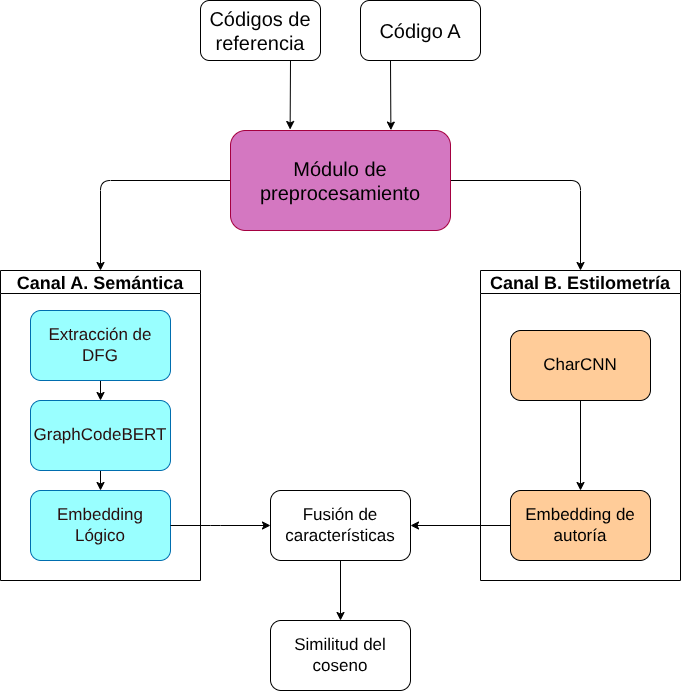
\includegraphics[width=0.8\textwidth]{figuras/diagrama_bloques.png} % Ajusta el ancho al 90% de la página
    \caption{Diagrama de bloques funcional del sistema de comparación Graphito.}
    \label{fig:diagrama_bloques} % Esta es la "etiqueta" para referenciarlo
\end{figure}

A continuación, se describen los componentes core que integran la solución:


%%%%%%%%%%%%%%%%%%%%%%%%%%%%%%%%%%%%%%%%%%%%%%%%%%%%%%%%%%%%%%%%%%%%%%%%%%%%%%%%%%%%
\subsection{Entrada de datos y fuentes de referencia}

El proceso de comparación comienza con la recepción de dos flujos de información fundamentales:

\begin{itemize}
    \item \textbf{Entrega del Alumno:} Archivos en formato fuente (.c o .cpp) que contienen la resolución propuesta por el estudiante a un problema en específico. El sistema está diseñado para procesar código basado en los estándares C11 y C++17, enfocandose en temas introductorios a la programacion como fundamentos y algoritmos y estructuras de datos. 
    
    \item \textbf{Códigos de Referencia:} Representan el conjunto de comparación, representando una o múltiples soluciones correctas al problema planteado. Este repositorio incluye la solución ideal proporcionada por el docente y, de manera complementaria, un conjunto de variantes funcionalmente equivalentes obtenidas mediante modelos de lenguaje (LLM). Esta diversidad de referencias permite que el sistema realice un cotejo robusto contra múltiples implementaciones lógicas de un mismo problema.
\end{itemize}

%%%%%%%%%%%%%%%%%%%%%%%%%%%%%%%%%%%%%%%%%%%%%%%%%%%%%%%%%%%%%%%%%%%%%%%%%%%%%%%%%%%%%%

\subsection{Módulo de Preprocesamiento y Normalización}

Una vez ingresados los archivos, el \textbf{Módulo de Preprocesamiento} genera dos representaciones distintas a partir de un mismo archivo fuente para satisfacer los requerimientos de cada canal de análisis:

\begin{enumerate}
    \item \textbf{Representación Normalizada (Canal A):} Se realiza una limpieza profunda de ambos conjuntos de código, eliminando comentarios, metadatos y espacios en blanco redundantes. Asimismo, se aplican técnicas de normalización de identificadores. Este proceso garantiza que el análisis semántico se enfoque exclusivamente en la topología del flujo de datos y la lógica algorítmica, ignorando cambios estéticos o de nomenclatura.
    \item \textbf{Representación Estructural/Raw (Canal B):} Se aplica únicamente a la solución del alumno. El sistema preserva elementos como la indentación, el uso de comentarios, la acentuación y caracteres especiales. Esta decisión técnica es clave para la detección de patrones de generación por IA, ya que permite identificar la "perfección" gramatical y hábitos de formato que constituyen la "huella digital" del autor o del modelo generativo utilizado.
\end{enumerate}

Una vez terminado ambos procesos, el flujo sigue hacia los canales de comparación semántica y analisis estilometríco. 

%%%%%%%%%%%%%%%%%%%%%%%%%%%%%%%%%%%%%%%%%%%%%%%%%%%%%%%%%%%%%%%%%%%
% 7.2 CANAL A: COMPARACIÓN SEMÁNTICA
%%%%%%%%%%%%%%%%%%%%%%%%%%%%%%%%%%%%%%%%%%%%%%%%%%%%%%%%%%%%%%%%%%%
\subsection{Canal A: Comparación Semántica}

Este canal constituye el componente principal para la identificación de equivalencias lógicas profundas, permitiendo detectar clones de código que comparten el mismo propósito algorítmico a pesar de presentar variaciones sintácticas. 

\subsubsection{Justificación y Selección del Modelo}

La selección de \textbf{GraphCodeBERT} \cite{Guo2021GraphCodeBERT} como motor de análisis semántico responde a la necesidad de superar las limitaciones de los modelos puramente secuenciales (como CodeBERT o Transformers estándar). La decisión se fundamenta en los siguientes pilares técnicos:

\begin{itemize}
    \item \textbf{Integración Estructural:} A diferencia de otros modelos que tratan el código como una simple secuencia de texto, GraphCodeBERT integra información estructural mediante el uso de grafos de flujo de datos (DFG). Esto permite que el mecanismo de atención se centre en las conexiones que tienen sentido semántico real.
    \item \textbf{Resistencia a la Ofuscación:} Debido a que el modelo captura la relación entre variables (\textit{def-use chains}), es altamente efectivo detectando similitudes incluso cuando el código ha sido alterado mediante cambios de nombres de variables, reordenamiento de sentencias o cambios en las estructuras de control.
    \item \textbf{Especialización Funcional:} Como se detalla en el marco teórico, este modelo se especializa en el comportamiento lógico del programa. Si bien tiende a ignorar rasgos superficiales como el estilo, esta característica se alinea perfectamente con la arquitectura bimodal de Graphito, delegando la responsabilidad del análisis de estilo al Canal B (CharCNN).
\end{itemize}



\subsubsection{Extracción de Grafo de Flujo de Datos (DFG)}

Un Grafo de Flujo de Datos (DFG) es una representación dirigida que captura las dependencias funcionales entre las variables de un programa mediante la identificación de sus relaciones de definición y uso (\textit{def-use chains}). De acuerdo con la metodología propuesta por Guo et al. \cite{Guo2021GraphCodeBERT}, los pasos para obtener esta representación son:

\begin{enumerate}
    \item \textbf{Generación del AST (Análisis sintáctico):} El código fuente se procesa para construir su Árbol de Sintaxis Abstracta (AST), obteniendo la jerarquía gramatical del programa.
    \item \textbf{Identificación de la secuencia de variables:} Se analizan los nodos terminales (hojas) del AST para extraer todas las variables presentes, preservando su orden de aparición.
    \item \textbf{Definición de los nodos del grafo:} Cada ocurrencia de una variable se establece como un nodo individual dentro del grafo.
    \item \textbf{Construcción de las aristas (Dependencias de valor):} Se trazan enlaces dirigidos entre nodos $v_i$ y $v_j$ si el valor de la variable $v_j$ depende directamente de la definición o valor previo de $v_i$.
\end{enumerate}

\subsubsection{Procesamiento en GraphCodeBERT}

Una vez construido el DFG, la secuencia de \textit{tokens} del código y la estructura del grafo se integran en el modelo. La arquitectura utiliza tareas de entrenamiento como la predicción de relaciones entre nodos, lo que favorece el aprendizaje de representaciones mucho más estructuradas y fieles al comportamiento funcional del software.

\subsubsection{Embedding Lógico}

El resultado final de este canal es un \textbf{Embedding Semántico}: un vector denso de alta dimensionalidad que actúa como una firma lógica del programa. Este vector permite realizar comparaciones de proximidad matemática, identificando si dos soluciones son funcionalmente iguales sin importar la forma en que fueron escritas.
%%%%%%%%%%%%%%%%%%%%%%%%%%%%%%%%%%%%%%%%%%%%%%%%%%%%%%%%%%%%%%%%%%%%%%%%%%%%%%%%%%%%%%%%%%%%%%%%%%%%

\subsection{Canal B: Comparación Estilométrica}

Mientras que el Canal A se encarga de la profundidad lógica, el Canal B se enfoca en la superficie del código. Para esta tarea, se seleccionó el modelo \textbf{CharCNN} \cite{Zhang2015CharCNN} sobre otras arquitecturas de procesamiento de lenguaje natural más complejas por una razón de eficiencia y diseño: al contar ya con un modelo de alta capacidad para el análisis semántico, no es necesario un segundo modelo que intente comprender la sintaxis global. En su lugar, se requiere un extractor de rasgos que sea capaz de ``ver'' el código como una señal visual.

\subsubsection{Justificación y Selección del Modelo}

La elección de una Red Neuronal Convolucional a nivel de caracteres (CharCNN) responde a su capacidad innata para actuar como un escáner de patrones locales. Dado que las CNN son especialistas en visión computacional, al aplicarlas al código fuente ``en bruto'' (\textit{raw code}), el modelo puede identificar automáticamente rasgos que para otros sistemas serían invisibles:

\begin{itemize}
    \item \textbf{Estilo como Señal Visual:} El modelo interpreta la indentación, el uso de espacios y la disposición de caracteres especiales como texturas visuales, permitiendo aprender el estilo del autor sin necesidad de conocer la gramática del lenguaje C++.
    \item \textbf{Detección de Hiper-perfección:} Mientras que un estudiante suele presentar una escritura heterogénea y con errores humanos de formato, los modelos de lenguaje (LLM) generan código con una estructura y puntuación gramaticalmente perfecta en los comentarios. CharCNN es ideal para detectar esta ``perfección'' sintética que delata el uso de IA.
    \item \textbf{Eficiencia Computacional:} Al operar localmente sobre secuencias de caracteres, el modelo aporta una capa de seguridad adicional sin incrementar drásticamente la carga computacional del sistema \textit{backend}.
\end{itemize}



\subsubsection{Análisis de Autoría mediante CharCNN}

El procedimiento estructurado para transformar el código fuente en un identificador de estilo se detalla a continuación:

\begin{enumerate}
    \item \textbf{Preservación de Código Raw:} Se utiliza la versión del código que conserva comentarios, sangrías y acentuación, elementos que suelen ser eliminados en análisis tradicionales pero que son críticos para la detección de la firma del autor.
    \item \textbf{Mapeo de Caracteres:} El texto se transforma en una secuencia de índices numéricos basados en un alfabeto predefinido, permitiendo que la red procese el código como una señal discreta y medible.
    \item \textbf{Extracción Convolucional de Rasgos:} Se aplican filtros convolucionales de distintos tamaños para detectar ``n-gramas'' de caracteres. Esto permite identificar hábitos microscópicos, como la preferencia por ciertos operadores o la pulcritud en la redacción de comentarios.
    \item \textbf{Reducción de Dimensionalidad (Pooling):} Se seleccionan las características más relevantes detectadas por los filtros, consolidando los rasgos estilísticos más distintivos de la muestra analizada en una representación compacta.
\end{enumerate}

\subsubsection{Generación de Embedding de Autoría}

Una vez procesada la información por las capas convolucionales, el sistema genera un \textbf{Embedding de Autoría}. Este vector denso representa la ``huella digital'' del emisor, capturando las sutilezas que diferencian la redacción manual de un estudiante de la generación estandarizada de un LLM.

Este embedding es fundamental para Graphito, ya que permite alertar al docente cuando la lógica de un programa coincide con la de una referencia, pero el estilo de escritura sugiere una procedencia no humana. En términos prácticos, el Canal B actúa como el detector de anomalías que complementa el juicio semántico del Canal A.

%%%%%%%%%%%%%%%%%%%%%%%%%%%%%%%%%%%%%%%%%%%%%%%%%%%%%%%%%%%%%%%%%%%%%%%%%%%%%%%%%%%%%%%%%%%%%%%%%%%%%
\subsection{Fusión de Características}

La fusión de características \cite{MartinezGil2026Improving} representa el proceso de integración donde las salidas de los canales semántico y estilométrico convergen para formar una representación única y bimodal de la entrega. 

Este bloque técnico es fundamental para el sistema Graphito, ya que permite consolidar dos dimensiones de análisis distintas en un solo espacio vectorial:

\begin{itemize}
    \item \textbf{Mecanismo de Integración:} El sistema toma el \textbf{Embedding Semántico} (que encapsula la lógica extraída por GraphCodeBERT) y el \textbf{Embedding de Autoría} (que contiene los rasgos estructurales detectados por CharCNN) y los combina mediante una operación de concatenación. En el caso de las soluciones de referencia, se aplica un acolchado de ceros (\textit{zero-padding}) en las dimensiones correspondientes al canal estilométrico, garantizando la homogeneidad dimensional necesaria para el cálculo de similitud.
    
    \item \textbf{Generación de la Firma Bimodal:} El resultado de esta fusión es un vector de características unificado que actúa como una "firma digital" del código. Esta firma no solo describe qué funciones realiza el programa, sino que también preserva los hábitos de escritura y formato del emisor.
\end{itemize}

Al integrar ambos tipos de información, la fusión permite que el sistema tenga una comprensión profunda del código, facilitando la detección de anomalías donde la lógica del programa es correcta pero el estilo de redacción es inconsistente con el perfil esperado, lo que constituye un indicio clave de asistencia por inteligencia artificial.

%%%%%%%%%%%%%%%%%%%%%%%%%%%%%%%%%%%%%%%%%%%%%%%%%%%%%%%%%%%%%%%%%%%
% 7.5 SIMILITUD DEL COSENO
%%%%%%%%%%%%%%%%%%%%%%%%%%%%%%%%%%%%%%%%%%%%%%%%%%%%%%%%%%%%%%%%%%%
\subsection{Similitud del Coseno}

La Similitud del Coseno es una métrica matemática que mide el coseno del ángulo entre dos vectores en un espacio multidimensional. A diferencia de otras métricas de distancia, esta no se ve afectada por la magnitud de los vectores (en este caso, la longitud del código), sino por su orientación, lo que la hace ideal para comparar la esencia de dos fragmentos de software.

La similitud entre la entrega del alumno ($A$) y el código de referencia ($R$) se calcula mediante la siguiente fórmula:

\begin{equation}
\text{sim}(A, R) = \frac{A \cdot R}{\|A\| \|R\|} = \frac{\sum_{i=1}^{n} A_i R_i}{\sqrt{\sum_{i=1}^{n} A_i^2} \sqrt{\sum_{i=1}^{n} R_i^2}}
\label{eq:coseno}
\end{equation}

El resultado de esta operación oscila en el intervalo $[0, 1]$, donde $1$ representa una coincidencia total de orientación y $0$ una independencia absoluta entre los vectores.

\subsubsection{Importancia de la Métrica en la Fusión de Características}

El uso de esta métrica es fundamental en Graphito debido a la naturaleza asimétrica de la fusión de características. Al combinar el análisis semántico (lógica) y el estilométrico (IA), la similitud del coseno actúa no solo como un comparador, sino como un regulador de integridad académica.



La relevancia de utilizar este enfoque bimodal radica en los siguientes puntos:

\begin{itemize}
    \item \textbf{Efecto de la Carga Estilística:} Para el sistema, el código del profesor es el "estándar de verdad", por lo que su vector se proyecta con una componente de estilo neutra. Si un alumno entrega un código con lógica perfecta pero generado por una IA, su vector adquirirá una "carga extra" en la dimensión del estilo.
    \item \textbf{Desviación del Vector:} Aunque el código del alumno sea funcionalmente idéntico al del profesor, la presencia de rasgos sintéticos (detectados por el Canal B) hace que el vector del alumno se "desvíe" o rote respecto al del profesor. Esta desviación incrementa el ángulo entre ambos, reduciendo automáticamente el valor de la similitud final.
    \item \textbf{Penalización Intrínseca:} Gracias a la propiedad del denominador en la fórmula (la norma del vector $\|A\|$), cualquier rastro de IA detectado incrementa la magnitud del vector del alumno sin aportar al numerador. Esto castiga la calificación de similitud de manera proporcional a la "perfección" sintética detectada, permitiendo diferenciar entre un alumno que programó honestamente y uno que utilizó asistencia externa.
\end{itemize}

En conclusión, la Similitud del Coseno permite que Graphito entregue un veredicto más justo y profundo. No se limita a decir si el programa "funciona igual", sino que evalúa si la forma en que fue construido se alinea con el estándar humano de referencia, convirtiéndola en una métrica esencial para combatir el plagio moderno potenciado por inteligencia artificial.


\section{Conclusión}

La propuesta de solución presentada en este capítulo, denominada \textbf{Graphito}, se aleja de los enfoques de comparación de texto tradicionales para adoptar una arquitectura bimodal basada en aprendizaje profundo. A través de la integración del análisis semántico (Canal A) y el análisis estilométrico (Canal B), el sistema es capaz de evaluar el código fuente no solo por lo que hace, sino por la identidad de su escritura.

La principal fortaleza de esta propuesta reside en su capacidad de autorregulación mediante la similitud del cosenos asimétrica. Al tratar la lógica como el eje central y el estilo como un factor de penalización, Graphito ofrece una métrica de integridad académica robusta frente a las técnicas modernas de ofuscación y la generación sintética por modelos de lenguaje. 

Con la definición funcional de estos bloques y la fundamentación de sus componentes core, queda establecida la base teórica y metodológica de la solución. En el siguiente capítulo, se procederá con el Anal   , donde se detallará la arquitectura de software, la persistencia de datos y los diagramas de interacción necesarios para la implementación física de esta propuesta.

\chapter{Análisis del Sistema}

\section{Análisis de Requerimientos}

En esta sección se describen los requerimientos funcionales y no funcionales del sistema propuesto, los cuales establecen las capacidades, restricciones y criterios de desempeño que debe cumplir la solución desarrollada. Estos requerimientos sirven como base para el diseño, implementación y evaluación del sistema, asegurando la trazabilidad entre las necesidades del evaluador y la arquitectura final.

% =========================================================
\subsection{Requerimientos Funcionales}
% =========================================================

Los requerimientos funcionales definen las capacidades y procesos que el sistema debe implementar para cumplir con las funciones de análisis, gestión de información y auditoría de código en el contexto académico.

\begin{itemize}
    \item \textbf{RF-01:} El sistema debe permitir el registro e inicio de sesión de docentes mediante credenciales cifradas para garantizar un espacio de trabajo privado.
    
    \item \textbf{RF-02:} El sistema debe permitir al docente la creación y gestión de un listado de ejercicios o problemas de programación (Biblioteca).
    
    \item \textbf{RF-03:} El sistema debe permitir la carga de código fuente en formato .c y .cpp asociados a un ejercicio específico.
    
    \item \textbf{RF-04:} El sistema debe realizar el preprocesamiento y normalización del código fuente, asegurando la correcta extracción de los grafos para el canal semántico, mientras se preserva la integridad de las estructuras de estilo originales para el detección de patrones generativos.
    
    \item \textbf{RF-05:} El sistema debe generar representaciones basadas en Grafos de Flujo de Datos (DFG) para el módulo semántico, y transformar el código fuente en secuencias matriciales bidimensionales (carácter por vector) para su procesamiento mediante convoluciones 1D en el módulo estilométrico.
    
    \item \textbf{RF-06:} El sistema debe realizar el análisis de similitud semántica mediante el modelo GraphCodeBERT para la generación de vectores de características (embeddings), cuantificando la proximidad entre ellos utilizando la métrica de similitud del coseno.
    
    \item \textbf{RF-07:} El sistema debe realizar el análisis estilométrico mediante el modelo CharCNN para calcular la probabilidad de generación mediante inteligencia artificial. sintética o humana.
    
    \item \textbf{RF-08:} El sistema debe solicitar y recibir múltiples versiones funcionalmente equivalentes del problema proporcionado por el docente a través de un modelo LLM externo.
    
    \item \textbf{RF-09:} El sistema debe realizar el almacenamiento persistente de los resultados del análisis y metadatos en una base de datos relacional (PostgreSQL), así como de los vectores de características en una base de datos vectorial (ChromaDB), asegurando la integridad referencial.
    
    \item \textbf{RF-10:} El sistema debe generar un reporte consolidado que integre el índice de similitud semántica y la probabilidad de generación mediante inteligencia artificial. de forma visual.
    
    \item \textbf{RF-11:} El sistema debe realizar una fusión de características (Feature Fusion) que integre el vector semántico y la probabilidad estilométrica, consolidando las métricas de ambos módulos en una sola estructura para su análisis dual.
    
    \item \textbf{RF-12:} El sistema debe permitir la consulta histórica de reportes de análisis realizados previamente sin necesidad de re-procesar los archivos fuente.
\end{itemize}

% =========================================================
\subsection{Requerimientos No Funcionales}
% =========================================================

Los requerimientos no funcionales establecen las restricciones, atributos de calidad y condiciones de desempeño que debe cumplir el sistema propuesto durante su operación.

\begin{itemize}
    \item \textbf{RNF-01:} Seguridad de datos: El sistema debe cifrar las contraseñas de los usuarios y utilizar tokens de sesión (JWT) para proteger la comunicación entre el cliente y el servidor.
    
    \item \textbf{RNF-02:} Persistencia híbrida: El sistema debe operar bajo un esquema de base de datos dual, optimizando las consultas relacionales en PostgreSQL y las búsquedas por similitud vectorial en ChromaDB.
    
    \item \textbf{RNF-03:} Los modelos de IA integrados deben estar calibrados buscando alcanzar un objetivo de rendimiento base de F1-Score $\ge$ 0.85 para GraphCodeBERT en tareas de detección de similitud semántica.
    
    \item \textbf{RNF-04:} El módulo estilométrico (CharCNN) debe estar optimizado para buscar una precisión de clasificación de autoría igual o superior a 0.8 bajo el corpus de pruebas establecido.
    
    \item \textbf{RNF-05:} El sistema debe soportar el análisis de código bajo los estándares C11 y C++17 para garantizar compatibilidad operativa con el currículo y las entregas esperadas.
    
    \item \textbf{RNF-06:} El orquestador de métricas debe ajustar los umbrales de decisión con el objetivo de mantener una tasa de falsos positivos menor al 10\% durante el análisis de doble canal.
    
    \item \textbf{RNF-07:} El tiempo de procesamiento de inferencia en el backend durante la fase de análisis de una entrega estudiantil no debe exceder los 20 segundos, dado que la indexación de referencias y la generación de variantes (LLM) se realizan de forma asíncrona en la fase de configuración previa.
    
    \item \textbf{RNF-08:} El sistema debe ser compatible para su ejecución en navegadores web basados en el motor Chromium versión 110 o superior.
    
    \item \textbf{RNF-09:} La interfaz web debe ser intuitiva, permitiendo ejecutar todas las tareas en 3 o menos acciones y proporcionar retroalimentación visual o indicadores de estado en tiempo real mientras el orquestador (LangGraph) procesa las tareas en segundo plano.
    
    \item \textbf{RNF-10:} El sistema debe asegurar alta disponibilidad operativa durante el procesamiento y análisis de código dentro del entorno de despliegue asignado para las pruebas.
    
    \item \textbf{RNF-11:} El sistema debe realizar validaciones preventivas en el cliente (tipo de archivo, tamaño e integridad) antes de iniciar la transmisión de la carga útil hacia la API REST.
\end{itemize}

% =========================================================
\subsection{Reglas de Negocio}
% =========================================================

Las reglas de negocio definen los criterios que guían el funcionamiento y uso ético del sistema dentro del entorno académico.

\begin{itemize}
    \item \textbf{RN-01:} Confidencialidad de los datos: Un docente solo podrá visualizar, editar y consultar los ejercicios y reportes generados bajo su propia cuenta de usuario.
    
    \item \textbf{RN-02:} El sistema se limita a programas de cursos de programación de ESCOM-IPN que sigan los estándares C11 y C++17.
    
    \item \textbf{RN-03:} Integridad de la referencia: Toda entrega debe ser comparada contra al menos una solución de referencia proporcionada por el docente para ser considerada válida.
    
    \item \textbf{RN-04:} La decisión final de calificación es responsabilidad exclusiva del docente; el sistema actúa únicamente como una herramienta objetiva de apoyo a la auditoría académica.
    
    \item \textbf{RN-05:} Se permite el uso de múltiples soluciones generadas por LLM para ampliar el espectro de comparación lógica, siempre que el docente las valide inicialmente.
    
    \item \textbf{RN-06:} Preservación de referencias: Los archivos cargados en calidad de entregas a analizar no podrán ser catalogados ni reutilizados por el sistema como códigos de referencia para futuras comparaciones, garantizando que el estándar de comparación se mantenga basado exclusivamente en soluciones validadas o generadas por el docente.
\end{itemize}

% =========================================================
\section{Identificación y descripción de actores}
% =========================================================

En el contexto del sistema propuesto (Graphito), los actores representan las entidades externas que interactúan con la plataforma y que participan en el flujo de configuración, análisis y auditoría del código fuente. La correcta identificación de estos actores permite definir los casos de uso, delimitar responsabilidades y establecer las fronteras del sistema.

A partir de la arquitectura funcional, se identifican exclusivamente dos actores que interactúan de forma directa con la plataforma:

% ---------------------------------------------------------
\subsection{Docente / Evaluador}
% ---------------------------------------------------------

Es el actor principal y humano del sistema. Utiliza la plataforma como una herramienta de apoyo a la decisión en su proceso de auditoría académica (correspondiente a profesores o instructores de programación).

Entre sus principales responsabilidades de interacción se encuentran:

\begin{itemize}
    \item Proporcionar la descripción técnica del problema o práctica.
    \item Configurar el marco de comparación cargando sus códigos de referencia.
    \item Cargar los archivos fuente (\textit{.c, .cpp}) desarrollados por los estudiantes para su análisis.
    \item Interpretar los reportes visuales generados por el sistema, incluyendo los índices de similitud semántica y la probabilidad de generación mediante inteligencia artificial..
    \item Tomar la decisión final sobre la calificación del alumno, utilizando la evidencia estática proporcionada por la herramienta.
\end{itemize}

% ---------------------------------------------------------
\subsection{Motor de Inteligencia Artificial Externo (LLM)}
% ---------------------------------------------------------

Este actor corresponde a una API de un sistema externo basado en Modelos de Lenguaje Grande (LLM). Actúa como un proveedor de servicios de generación de código sintético bajo demanda.

Sus funciones en interacción con el orquestador de Graphito son:

\begin{itemize}
    \item Recibir el código de referencia original y generar descripciones técnicas algorítmicas.
    \item Generar múltiples variantes de código que sean funcionalmente equivalentes a la referencia del docente.
    \item Proveer el insumo necesario para que el sistema indexe un espacio vectorial de comparación mucho más robusto.
\end{itemize}

% =========================================================
\section{Trayectorias principales y alternativas}
% =========================================================

Las trayectorias describen el flujo de interacción entre el docente, el orquestador backend y los modelos de IA, detallando las secuencias de acciones para llevar a cabo el análisis bimodal. Estas trayectorias reflejan el comportamiento esperado (Modelado BPMN) y los escenarios alternativos.

% ---------------------------------------------------------
\subsection{Trayectoria principal (Flujo de Análisis Estándar)}
% ---------------------------------------------------------

La trayectoria principal describe el flujo de uso del sistema para procesar una entrega estudiantil contra referencias previamente configuradas.

\begin{enumerate}
    \item El docente accede a su biblioteca en la plataforma web del sistema.
    \item El docente carga el archivo fuente a analizar, seleccionando el problema correspondiente.
    \item El backend recibe el código y ejecuta el preprocesamiento y normalización (limpieza para el canal semántico y preservación de formato para el estilométrico).
    \item \textbf{Canal Semántico:} Se extrae el Grafo de Flujo de Datos (DFG) y el modelo \textit{GraphCodeBERT} genera el embedding estructural.
    \item \textbf{Canal Estilométrico:} El modelo \textit{CharCNN} procesa la matriz de caracteres 1D para estimar la probabilidad de generación mediante inteligencia artificial.
    \item El orquestador ejecuta la \textbf{Fusión de Características (Feature Fusion)} unificando ambos resultados.
    \item El sistema calcula la similitud del coseno del vector unificado contra la base de datos vectorial (\textit{ChromaDB}).
    \item El sistema consolida los resultados y persiste los metadatos en la base de datos relacional (\textit{PostgreSQL}).
    \item El sistema renderiza el reporte de análisis dual.
    \item El docente visualiza los indicadores numéricos y toma una decisión informada.
\end{enumerate}

% ---------------------------------------------------------
\subsection{Trayectorias alternativas}
% ---------------------------------------------------------

Las trayectorias alternativas describen variaciones del flujo principal, orquestadas por \textit{LangGraph} ante condiciones específicas.

\textbf{A1. Robustecimiento de referencias mediante LLM}

\begin{enumerate}
    \item Durante la configuración de un problema, el docente solicita la generación de variantes de su solución.
    \item El sistema envía el código de referencia al LLM externo.
    \item El modelo externo retorna múltiples soluciones equivalentes.
    \item El sistema calcula los embeddings semánticos de estas variantes y los indexa en la base vectorial de forma asíncrona.
\end{enumerate}

\textbf{A2. Código con errores críticos de formato}

\begin{enumerate}
    \item El sistema detecta inconsistencias irreparables durante la normalización inicial del código.
    \item El orquestador detiene el flujo antes de la inferencia de los modelos.
    \item Se notifica al docente en la interfaz sobre la invalidez del archivo fuente.
\end{enumerate}

\textbf{A3. Análisis estilométrico de baja confianza}

\begin{enumerate}
    \item El sistema identifica que el código cargado carece de una extensión mínima para extraer patrones de caracteres viables.
    \item El orquestador reduce la ponderación del canal estilométrico en la fusión de características.
    \item El sistema prioriza el índice de similitud semántica y añade una nota técnica en el reporte final.
\end{enumerate}

\textbf{A4. Alta equivalencia lógica detectada}

\begin{enumerate}
    \item El cálculo de la similitud del coseno arroja un valor superior al umbral establecido.
    \item El sistema clasifica la entrega como de alto interés de auditoría.
    \item Se destaca visualmente el registro en el panel del docente para sugerir una revisión prioritaria.
\end{enumerate}

\textbf{A5. Discrepancia crítica en análisis de doble canal}

\begin{enumerate}
    \item El orquestador detecta una correlación anómala (ej. alta similitud lógica combinada con una huella de autoría clasificada como inteligencia artificial).
    \item El sistema estructura un indicador visual de inconsistencia en el reporte final.
    \item El docente analiza el reporte detallado para auditar la anomalía.
\end{enumerate}

\section{Diagrama de Casos de Uso}

El análisis de casos de uso define las fronteras del sistema Graphito y describe las interacciones entre los actores externos y las funcionalidades internas. Este modelo permite visualizar cómo el evaluador gestiona el proceso de auditoría académica, desde la configuración inicial hasta la toma de decisiones basada en el reporte bimodal.

En la Figura~\ref{fig:casos_uso} se presenta el diagrama de casos de uso general del sistema, estructurado de forma jerárquica para reflejar el flujo de trabajo del docente.

\begin{figure}[H]
    \centering
    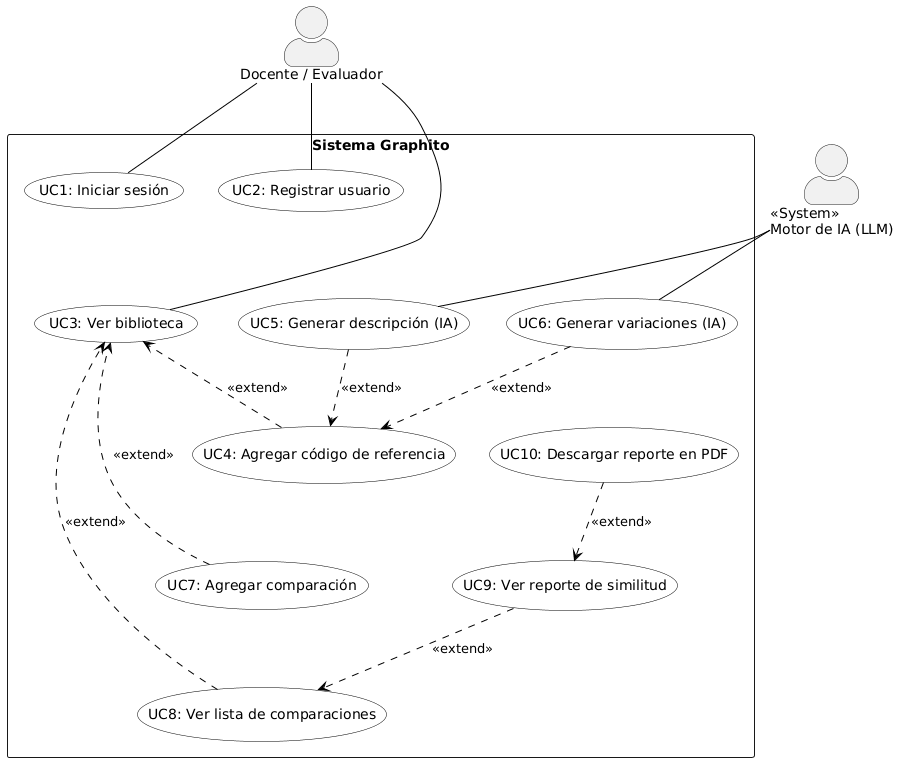
\includegraphics[width=0.75\textwidth]{figuras/casos_uso_v2.png} 
    \caption{Diagrama de casos de uso del sistema Graphito.}
    \label{fig:casos_uso}
\end{figure}

\subsection{Descripción de Actores}

Para el funcionamiento del sistema se han identificado dos actores principales:

\begin{itemize}
    \item \textbf{Docente / Evaluador:} Actor principal humano que interactúa con la plataforma para configurar problemas, gestionar entregas y visualizar los reportes de similitud.
    \item \textbf{Modelo LLM Externo:} Actor de sistema que actúa como proveedor de servicios de generación de código. Es consultado de forma opcional para robustecer el conjunto de referencias.
\end{itemize}

\subsection{Descripción de los Casos de Uso}

A continuación, se describen los módulos funcionales que integran la solución \textit{Graphito}, estructurados de acuerdo con su rol en el flujo de auditoría académica:

\begin{itemize}
    \item \textbf{Gestión de Acceso y Biblioteca (UC1, UC2, UC3):} Facilitan la administración de la sesión del docente y el acceso a la pagina principal (Biblioteca). Este módulo centraliza los ejercicios históricos y las comparaciones realizadas, permitiendo un entorno de trabajo persistente.
    \item \textbf{Gestión de Referencias y Pre-procesamiento (UC4, UC5, UC6, UC11):} Permiten al evaluador establecer el marco de comparación. Incluye la carga de soluciones base (UC4) y su enriquecimiento mediante un motor de IA externo para generar descripciones y variantes sintéticas (UC5, UC6). De forma obligatoria (\textit{include}), el sistema realiza la generación de \textit{embeddings} semánticos (UC11) sobre estas referencias.
    \item \textbf{Ejecución de Comparaciones (UC7, UC12):} Constituye el núcleo operativo del sistema. Al agregar una entrega para comparar (UC7), el sistema ejecuta automáticamente (\textit{include}) el análisis de doble canal (UC12), el cual integra el procesamiento semántico de flujo de datos y el detección de patrones generativos estilométrica.
    \item \textbf{Resultados y Reporteo (UC8, UC9, UC10):} Proporcionan la interfaz de auditoría donde se listan las comparaciones (UC8) y se visualizan los reportes de similitud detallados (UC9). Finalmente, se permite la exportación de resultados en formato PDF (UC10) para su integración en actas de evaluación.
\end{itemize}

\subsection{Especificación de Casos de Uso}

A continuación se detallan los casos de uso que rigen el comportamiento del sistema Graphito. Estas especificaciones describen la interacción detallada entre los actores y los módulos de inteligencia artificial.

% =========================================================
% ESPECIFICACIÓN DE CASOS DE USO
% =========================================================

% --- CASO DE USO 1 ---
\begin{table}[H]
\centering
\begin{tabular}{|p{3cm}|p{11cm}|}
\hline
\rowcolor[HTML]{E7F3FF} 
\textbf{Caso de Uso:} & \textbf{UC1: Iniciar sesión} \\ \hline
\textbf{Actor:} & Docente / Evaluador \\ \hline
\textbf{Descripción:} & El docente ingresa sus credenciales de acceso para entrar al sistema Graphito. \\ \hline
\textbf{Precondiciones:} & El docente debe estar registrado previamente en la plataforma (UC2). \\ \hline
\textbf{Flujo Básico:} & 
1. El docente ingresa su correo electrónico y contraseña en la interfaz. \newline
2. El sistema valida las credenciales mediante un proceso de autenticación cifrada contra la base de datos relacional (PostgreSQL). \newline
3. El sistema genera un token de sesión (JWT) y redirige al docente a su Biblioteca (UC3). \\ \hline
\textbf{Trayectorias Alternativas:} & Si las credenciales son incorrectas, el sistema muestra un mensaje de error y deniega el acceso, manteniendo la sesión cerrada. \\ \hline
\end{tabular}
\caption{Especificación del Caso de Uso 1.}
\end{table}

% --- CASO DE USO 2 ---
\begin{table}[H]
\centering
\begin{tabular}{|p{3cm}|p{11cm}|}
\hline
\rowcolor[HTML]{E7F3FF} 
\textbf{Caso de Uso:} & \textbf{UC2: Registrar usuario} \\ \hline
\textbf{Actor:} & Docente / Evaluador \\ \hline
\textbf{Descripción:} & Un nuevo docente crea una cuenta en la plataforma para poder gestionar sus ejercicios, referencias y comparaciones. \\ \hline
\textbf{Flujo Básico:} & 
1. El docente proporciona su nombre, correo electrónico y define una contraseña. \newline
2. El sistema cifra la contraseña y registra al nuevo usuario en PostgreSQL. \newline
3. El sistema confirma el registro exitoso y redirige a la vista de inicio de sesión. \\ \hline
\textbf{Postcondición:} & Se inicializa un espacio aislado en la base de datos para el repositorio personal del docente. \\ \hline
\end{tabular}
\caption{Especificación del Caso de Uso 2.}
\end{table}

% --- CASO DE USO 3 ---
\begin{table}[H]
\centering
\begin{tabular}{|p{3cm}|p{11cm}|}
\hline
\rowcolor[HTML]{E7F3FF} 
\textbf{Caso de Uso:} & \textbf{UC3: Ver biblioteca} \\ \hline
\textbf{Actor:} & Docente / Evaluador \\ \hline
\textbf{Descripción:} & Página principal del sistema donde el docente accede a su biblioteca personal, desde donde visualiza los problemas configurados previamente o inicia nuevas configuraciones. \\ \hline
\textbf{Precondiciones:} & El docente debe haber iniciado sesión de forma exitosa (UC1). \\ \hline
\textbf{Flujo Básico:} & 
1. El docente selecciona la opción de "Biblioteca" en la interfaz. \newline
2. El sistema recupera de PostgreSQL la lista de ejercicios asociados al identificador del docente. \newline
3. El sistema muestra la lista de ejercicios, habilitando las opciones de gestión (agregar referencia, ver comparaciones). \\ \hline
\textbf{Postcondición:} & El sistema queda a la espera de la ejecución de una acción extendida (UC4, UC7, UC8). \\ \hline
\end{tabular}
\caption{Especificación del Caso de Uso 3.}
\end{table}

% --- CASO DE USO 4 ---
\begin{table}[H]
\centering
\begin{tabular}{|p{3cm}|p{11cm}|}
\hline
\rowcolor[HTML]{E7F3FF} 
\textbf{Caso de Uso:} & \textbf{UC4: Agregar código de referencia} \\ \hline
\textbf{Actor:} & Docente / Evaluador \\ \hline
\textbf{Descripción:} & El docente carga el código fuente que servirá como solución ideal, inicializando el proceso asíncrono de indexación semántica. \\ \hline
\textbf{Precondiciones:} & El docente debe encontrarse gestionando un ejercicio dentro de la Biblioteca (UC3). \\ \hline
\textbf{Flujo Básico:} & 
1. El docente selecciona agregar una nueva referencia y carga el archivo (.c o .cpp). \newline
2. El sistema normaliza el código eliminando comentarios. \newline
3. El orquestador extrae el Grafo de Flujo de Datos (DFG) y genera el embedding correspondiente mediante GraphCodeBERT. \newline
4. El vector semántico resultante se almacena en ChromaDB. \newline
5. El sistema habilita las opciones para enriquecer la referencia utilizando un modelo de IA externo (UC5, UC6). \\ \hline
\textbf{Postcondición:} & El código base queda indexado en la base vectorial, preparado para futuras comparaciones. \\ \hline
\end{tabular}
\caption{Especificación del Caso de Uso 4.}
\end{table}

% --- CASO DE USO 5 ---
\begin{table}[H]
\centering
\begin{tabular}{|p{3cm}|p{11cm}|}
\hline
\rowcolor[HTML]{E7F3FF} 
\textbf{Caso de Uso:} & \textbf{UC5: Generar descripción (IA)} \\ \hline
\textbf{Actor:} & Motor de IA (LLM) / Docente \\ \hline
\textbf{Descripción:} & El sistema consume una API de LLM externo para redactar automáticamente un resumen o descripción técnica basada en la lógica del código de referencia. \\ \hline
\textbf{Precondiciones:} & Debe existir un código de referencia cargado en el sistema (UC4). \\ \hline
\textbf{Flujo Básico:} & 
1. El docente solicita la autogeneración de la descripción del problema. \newline
2. El sistema envía el código crudo al LLM empaquetado en un prompt específico de resumen algorítmico. \newline
3. El LLM devuelve la descripción técnica generada. \newline
4. El docente revisa el texto, realiza ajustes si lo considera necesario y confirma su guardado en los metadatos de PostgreSQL. \\ \hline
\end{tabular}
\caption{Especificación del Caso de Uso 5.}
\end{table}

% --- CASO DE USO 6 ---
\begin{table}[H]
\centering
\begin{tabular}{|p{3cm}|p{11cm}|}
\hline
\rowcolor[HTML]{E7F3FF} 
\textbf{Caso de Uso:} & \textbf{UC6: Generar variaciones (IA)} \\ \hline
\textbf{Actor:} & Motor de IA (LLM) / Docente \\ \hline
\textbf{Descripción:} & El sistema utiliza el LLM externo para generar variantes funcionalmente equivalentes al código base. \\ \hline
\textbf{Precondiciones:} & Se debe haber cargado exitosamente al menos un código de referencia manual (UC4). \\ \hline
\textbf{Flujo Básico:} & 
1. El docente solicita la generación de N variantes para robustecer las referencias, otorgando consideraciones para la generación de las mismas. \newline
2. El sistema envía el código de referencia y las consideraciones al LLM externo. \newline
3. El LLM retorna N versiones sintéticas del código con la lógica requerida. \newline
4. El sistema preprocesa estas variantes, genera sus respectivos embeddings semánticos a través de GraphCodeBERT y las indexa en ChromaDB. \\ \hline
\textbf{Trayectorias Alternativas:} & Si la API del LLM no responde o excede el tiempo límite, el sistema notifica al docente y finaliza el proceso manteniendo activa únicamente la referencia original. \\ \hline
\end{tabular}
\caption{Especificación del Caso de Uso 6.}
\end{table}

% --- CASO DE USO 7 ---
\begin{table}[H]
\centering
\begin{tabular}{|p{3cm}|p{11cm}|}
\hline
\rowcolor[HTML]{E7F3FF} 
\textbf{Caso de Uso:} & \textbf{UC7: Agregar comparación} \\ \hline
\textbf{Actor:} & Docente / Evaluador \\ \hline
\textbf{Descripción:} & El docente carga una entrega estudiantil para ser comparada con el repositorio de referencias indexadas, ejecutando el análisis de los modelos de Deep Learning. \\ \hline
\textbf{Precondiciones:} & El problema debe contar con al menos una referencia previamente indexada en ChromaDB. \\ \hline
\textbf{Flujo Básico:} & 
1. El docente carga el archivo (.c o .cpp) correspondiente a la entrega a evaluar. \newline
2. El sistema inicia la inferencia paralela: GraphCodeBERT calcula el vector lógico (semántico) y CharCNN calcula la probabilidad de generación mediante inteligencia artificial. sintética (estilométrico). \newline
3. El orquestador ejecuta la Fusión de Características (Feature Fusion) para consolidar las métricas de doble canal. \newline
4. Se ejecuta una búsqueda matemática de Similitud del Coseno contra los vectores indexados en ChromaDB. \newline
5. Los resultados se persisten en PostgreSQL vinculados exclusivamente al nombre del archivo analizado. \\ \hline
\textbf{Postcondición:} & La entrega finaliza la comparación y queda disponible para su consulta detallada (UC8). \\ \hline
\end{tabular}
\caption{Especificación del Caso de Uso 7.}
\end{table}

% --- CASO DE USO 8 ---
\begin{table}[H]
\centering
\begin{tabular}{|p{3cm}|p{11cm}|}
\hline
\rowcolor[HTML]{E7F3FF} 
\textbf{Caso de Uso:} & \textbf{UC8: Ver lista de comparaciones} \\ \hline
\textbf{Actor:} & Docente / Evaluador \\ \hline
\textbf{Descripción:} & El docente visualiza un panel con el listado general de todas las entregas que han completado su proceso de comparación para un ejercicio específico. \\ \hline
\textbf{Precondiciones:} & El docente debe haber seleccionado un ejercicio activo desde la Biblioteca (UC3). \\ \hline
\textbf{Flujo Básico:} & 
1. El docente accede a la pestaña de comparaciones del problema seleccionado. \newline
2. El sistema consulta en PostgreSQL los metadatos de los análisis vinculados a dicho ejercicio. \newline
3. El sistema despliega una tabla resumiendo los nombres de los archivos procesados y sus puntajes consolidados. \\ \hline
\textbf{Postcondición:} & El docente tiene la opción de seleccionar un archivo específico para abrir su reporte (UC9). \\ \hline
\end{tabular}
\caption{Especificación del Caso de Uso 8.}
\end{table}

% --- CASO DE USO 9 ---
\begin{table}[H]
\centering
\begin{tabular}{|p{3cm}|p{11cm}|}
\hline
\rowcolor[HTML]{E7F3FF} 
\textbf{Caso de Uso:} & \textbf{UC9: Ver reporte de similitud} \\ \hline
\textbf{Actor:} & Docente / Evaluador \\ \hline
\textbf{Descripción:} & El docente abre la vista detallada de una comparación, donde el sistema renderiza la interpretación matemática de los modelos de IA. \\ \hline
\textbf{Precondiciones:} & El docente seleccionó una entrega desde el listado de comparaciones (UC8). \\ \hline
\textbf{Flujo Básico:} & 
1. El docente selecciona un archivo evaluado. \newline
2. El sistema recupera el reporte de doble canal completo desde PostgreSQL. \newline
3. El sistema renderiza la interfaz mostrando de forma gráfica el índice de similitud semántica y la probabilidad de generación mediante inteligencia artificial. del código. \\ \hline
\end{tabular}
\caption{Especificación del Caso de Uso 9.}
\end{table}

% --- CASO DE USO 10 ---
\begin{table}[H]
\centering
\begin{tabular}{|p{3cm}|p{11cm}|}
\hline
\rowcolor[HTML]{E7F3FF} 
\textbf{Caso de Uso:} & \textbf{UC10: Descargar reporte en PDF} \\ \hline
\textbf{Actor:} & Docente / Evaluador \\ \hline
\textbf{Descripción:} & El docente exporta el reporte de doble canal de similitud a un documento estructurado, obteniendo una evidencia técnica estática e imprimible de la comparación. \\ \hline
\textbf{Precondiciones:} & El docente debe estar visualizando un reporte de similitud procesado (UC9). \\ \hline
\textbf{Flujo Básico:} & 
1. El docente ejecuta la acción "Descargar PDF" desde la interfaz del reporte. \newline
2. El backend compila el nombre del archivo, el gráfico de similitud, el índice estilométrico y los indicadores visuales detectados. \newline
3. El sistema genera un archivo en formato PDF aplicando una plantilla institucional. \newline
4. El sistema transmite el archivo para su descarga directa en el dispositivo local del evaluador. \\ \hline
\textbf{Postcondición:} & El flujo de auditoría académica concluye satisfactoriamente con la generación de la evidencia estática. \\ \hline
\end{tabular}
\caption{Especificación del Caso de Uso 10.}
\end{table}

\section{Modelado de Procesos de Negocio (BPMN)}

Para la orquestación de las capacidades de inteligencia artificial y la gestión de la persistencia híbrida, se diseñó un modelo de procesos utilizando la notación BPMN 2.0. Este modelo, ilustrado en la Figura \ref{fig:bpmn_proceso}, detalla la interacción entre el docente, el motor de \textit{backend} y los módulos de inferencia de IA.

El proceso se divide en tres áreas de responsabilidad (\textit{lanes}) claramente definidas:

\begin{itemize}
    \item \textbf{Usuario (Docente):} Responsable de la carga de archivos de referencia y entrega, y la toma de decisiones basada en los reportes generados.
    \item \textbf{Backend:} Actúa como el orquestador del sistema, gestionando la validación de archivos, la comunicación con las bases de datos (relacional y vectorial) y la sincronización de los flujos de datos.
    \item \textbf{Módulo de IA:} Ejecuta las tareas de cómputo intensivo, incluyendo la generación de variantes sintéticas mediante LLMs, la extracción de características semánticas con \textit{GraphCodeBERT} y el análisis estilométrico mediante convoluciones 1D (\textit{CharCNN}).
\end{itemize}

\subsection{Descripción del Flujo de Trabajo}

El ciclo operativo de \textit{Graphito} se desglosa en tres fases críticas:

\begin{enumerate}
    \item \textbf{Fase de Gestión de Referencias:} El sistema ofrece caminos de ejecución alternativos para establecer la base de comparación. Si la configuración del problema es nueva, el \textit{backend} verifica su existencia en la base de datos relacional; en caso de no existir, el módulo de IA genera variantes sintéticas para robustecer el espacio vectorial. Si la referencia ya existe, se recupera directamente su representación densa (\textit{embedding}) desde la base de datos vectorial (\textit{ChromaDB}), optimizando los tiempos de respuesta.
    
    \item \textbf{Fase de Análisis de Doble Canal:} Una vez cargado el código a comparar, el sistema realiza un pre-procesamiento y normalización en el \textit{backend}. Posteriormente, el flujo se bifurca mediante una compuerta paralela para realizar un análisis dual: una extracción de lógica estructural (semántica) y un análisis de patrones de escritura (estilometría). Esta fase garantiza que el sistema capture tanto la intención funcional como la huella de autoría sintética o humana.
    
    \item \textbf{Fase de Fusión y Resultados:} Los vectores resultantes son integrados en un proceso de fusión de características (\textit{Feature Fusion}). El sistema utiliza una compuerta de sincronización para asegurar que tanto el vector consolidado del archivo analizado como el vector de la referencia estén disponibles de forma concurrente antes de calcular la \textit{Similitud del Coseno}. Finalmente, el módulo de IA interpreta los resultados numéricos para estructurar un reporte técnico que se persiste en el historial y se presenta al docente.
\end{enumerate}

\begin{figure}[H]
    \centering
    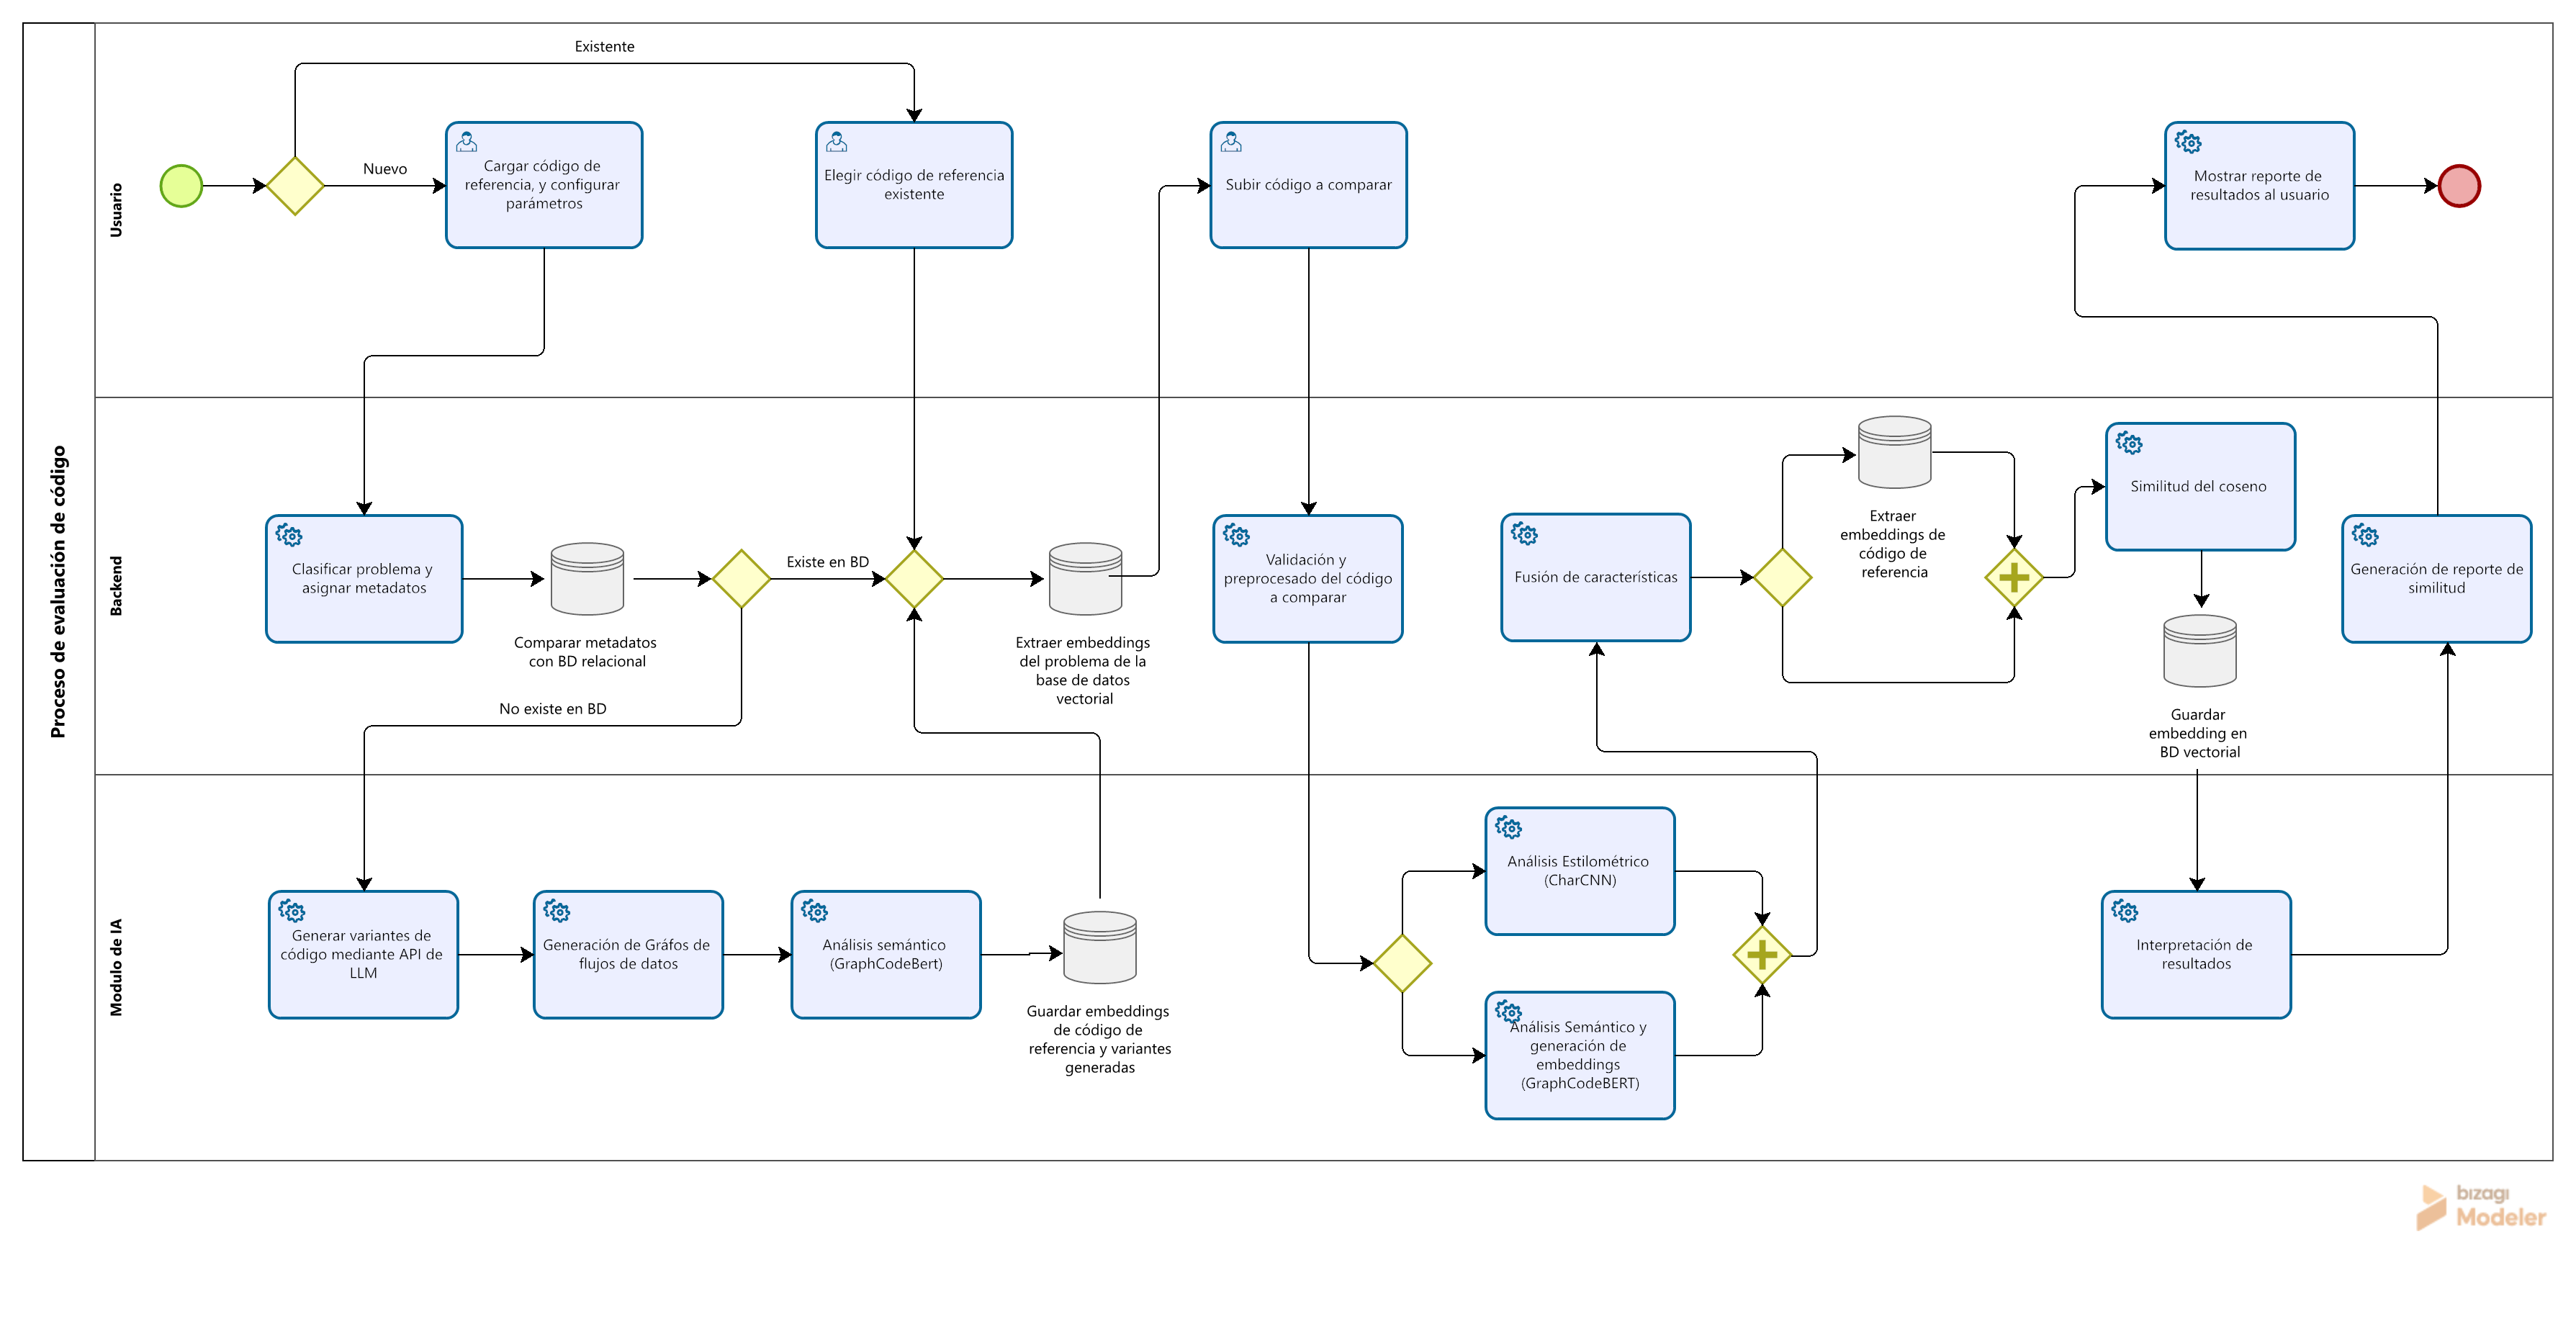
\includegraphics[width=\textwidth]{figuras/ModeloBPMN.png}
    \caption{Diagrama BPMN de la comparación de código fuente.}
    \label{fig:bpmn_proceso}
\end{figure}

% ---------------------------------------------------------
\section{Características semánticas del código}
% ---------------------------------------------------------

A diferencia del análisis estilométrico, el análisis semántico se centra en la lógica subyacente y la funcionalidad del programa, ignorando aspectos superficiales como el nombre de las variables o el formato del texto. Estas características permiten capturar la esencia algorítmica de una solución, lo que facilita la identificación de códigos que, aunque parezcan diferentes visualmente, ejecutan la misma lógica de resolución.

En la Tabla~\ref{tab:caracteristicas_semanticas} se presenta una clasificación de las características semánticas identificadas para la construcción de la firma lógica en este proyecto.

\begin{table}[H]
\centering
\small 
\begin{tabularx}{\textwidth}{l l X}
\toprule
\textbf{Categoría} & \textbf{Característica} & \textbf{Descripción Sintetizada} \\
\midrule
\textbf{Flujo de Datos} & Def-Uso & Rastreo del ciclo de vida y uso de variables. \\
                        & Dependencias & Vínculos lógicos entre variables y operaciones. \\
\midrule
\textbf{Lógica de}      & Caminos & Rutas lógicas y bifurcaciones del algoritmo. \\
\textbf{Control}        & Estructuras & Patrones de repetición y decisiones funcionales. \\
\midrule
\textbf{Representación} & AST / DFG & Jerarquía gramatical y grafo de flujo de datos. \\
\textbf{Estructural}    & Scope & Contexto de validez de las entidades lógicas. \\
\midrule
\textbf{Contexto}       & Semántica & Significado de tokens según su entorno. \\
                        & Equivalencia & Funcionalidad idéntica con distinta sintaxis. \\
\bottomrule
\end{tabularx}
\caption{Clasificación sintetizada de características semánticas del código.}
\label{tab:caracteristicas_semanticas}
\end{table}

La extracción de estas características permite generar una representación robusta ante técnicas de ofuscación comunes, como el renombrado de variables o el cambio de estructuras de control equivalentes (por ejemplo, sustituir un ciclo \textit{for} por un \textit{while}). En este sistema, el uso de \textit{GraphCodeBERT} es fundamental, ya que este modelo no solo procesa el código como una secuencia de texto, sino que incorpora explícitamente el Grafo de Flujo de Datos (DFG). Esto permite que las representaciones vectoriales resultantes capturen de manera profunda las dependencias lógicas, facilitando un análisis semántico preciso incluso cuando la estructura superficial ha sido alterada intencionalmente.

% ---------------------------------------------------------
\section{Características estilométricas del código}
% ---------------------------------------------------------

Para el canal de análisis estilométrico, se identifican diferentes tipos de características que permiten capturar patrones asociados a la escritura del autor. Estas características no dependen de la funcionalidad del programa, sino de la huella digital sintáctica y de formato, lo que permite distinguir entre diferentes autores o identificar probables intervenciones de generación sintética (IA).

En la Tabla~\ref{tab:caracteristicas_estilometricas} se presenta una clasificación de las principales características estilométricas que la red neuronal procesa de forma implícita.

\begin{table}[H]
\centering
\small
\begin{tabular}{lll}
\toprule
\textbf{Categoría} & \textbf{Característica} & \textbf{Descripción} \\
\midrule
Léxicas & Frecuencia de caracteres & Distribución de caracteres y símbolos en el código. \\
        & Uso de palabras clave & Frecuencia de keywords del lenguaje (C11/C++17). \\
        & Longitud de tokens & Tamaño promedio de identificadores y expresiones. \\
\midrule
Sintácticas & Estructuras de control & Preferencia de uso entre if, for, while, switch. \\
            & Anidamiento & Profundidad promedio de los bloques de código. \\
            & Modularidad & Tendencia en la organización en funciones o bloques. \\
\midrule
Formato & Indentación & Uso predominante de espacios o tabulaciones. \\
        & Saltos de línea & Patrones de densidad y distribución de líneas. \\
        & Estilo de llaves & Ubicación de apertura y cierre de bloques \{ \}. \\
\midrule
Estructurales & Tamaño del código & Número total de líneas del archivo original. \\
              & Uso de comentarios & Densidad y ubicación de comentarios respecto al código. \\
\bottomrule
\end{tabular}
\caption{Clasificación de características estilométricas del código fuente.}
\label{tab:caracteristicas_estilometricas}
\end{table}

Estas características permiten construir una representación del estilo de codificación que puede ser utilizada por modelos de aprendizaje automático para identificar anomalías de autoría. En particular, los modelos basados en redes neuronales convolucionales a nivel de caracteres (CharCNN) son capaces de aprender automáticamente patrones locales y distribuciones espaciales en la secuencia de caracteres cruda (preservando el estilo y formato original), lo que resulta especialmente útil para capturar diferencias sutiles entre código escrito por un estudiante humano y código generado de forma automatizada.

% =========================================================
\section{Definición de métricas de desempeño}
% =========================================================

La validación del sistema propuesto requiere la definición de métricas cuantitativas que permitan medir el desempeño algorítmico en los distintos módulos que lo componen. En particular, se consideran los dos componentes de la arquitectura dual: el canal de similitud semántica y el canal de análisis estilométrico.

Cada uno de estos módulos requiere métricas específicas que permitan evaluar su precisión, confiabilidad y utilidad computacional, permitiendo así validar la efectividad de la herramienta como apoyo objetivo a la auditoría docente.

% ---------------------------------------------------------
\subsection{Métricas para el análisis de similitud semántica}
% ---------------------------------------------------------

El canal de análisis semántico tiene como objetivo cuantificar el grado de equivalencia lógica entre dos programas. Para ello, se utilizan representaciones vectoriales (embeddings) generadas mediante el modelo \textit{GraphCodeBERT}.

La principal métrica utilizada es la similitud del coseno, la cual mide el ángulo entre dos vectores en un espacio de alta dimensión. Su valor se encuentra en el rango de [-1, 1], donde valores cercanos a 1 indican una alta proximidad entre los grafos lógicos de los programas analizados.

Esta métrica resulta especialmente adecuada para comparar embeddings, ya que permite determinar la cercanía semántica entre soluciones de software independientemente de su estructura sintáctica superficial.

Adicionalmente, se considera la correlación con el juicio experto como un mecanismo de validación externa, con el fin de determinar si los índices matemáticos generados por el sistema son consistentes con la auditoría manual del evaluador.

% ---------------------------------------------------------
\subsection{Métricas para el análisis estilométrico}
% ---------------------------------------------------------

El canal estilométrico, impulsado por la red neuronal \textit{CharCNN}, se plantea como un problema de clasificación binaria, en el cual se infiere si un fragmento de código presenta patrones de escritura correspondientes a un humano o a generación sintética mediante inteligencia artificial.

Para evaluar el desempeño de este modelo de Deep Learning, se utilizan métricas estándar de clasificación supervisada:

\begin{itemize}
    \item \textbf{Accuracy (Exactitud)}: mide la proporción de predicciones correctas respecto al total de muestras analizadas.
    \item \textbf{Precision (Precisión)}: indica la proporción de predicciones positivas correctas respecto al total de predicciones positivas realizadas.
    \item \textbf{Recall (Exhaustividad)}: mide la capacidad del modelo para identificar correctamente todos los casos positivos reales.
    \item \textbf{F1-score}: representa la media armónica entre precisión y exhaustividad, proporcionando una medida equilibrada del desempeño del modelo ante posibles desbalances de clases.
\end{itemize}

Estas métricas permiten calibrar el comportamiento del modelo en distintos escenarios, particularmente para minimizar la tasa de falsos positivos al detectar anomalías de autoría.

% ---------------------------------------------------------
\subsection{Resumen de métricas utilizadas}
% ---------------------------------------------------------

En la Tabla~\ref{tab:resumen_metricas} se presenta un resumen de las métricas empleadas en cada uno de los módulos de la arquitectura.

\begin{table}[H]
\centering
\begin{tabular}{lll}
\toprule
\textbf{Módulo} & \textbf{Métrica} & \textbf{Propósito} \\
\midrule
Similitud semántica & Similitud del coseno & Medir cercanía espacial entre embeddings. \\
                    & Correlación humana & Validar coherencia con la auditoría docente. \\
\midrule
Análisis estilométrico & Accuracy & Evaluar desempeño general de la red CharCNN. \\
                       & Precision & Medir exactitud en alertas de autoría. \\
                       & Recall & Evaluar detección de anomalías sintéticas. \\
                       & F1-score & Balancear rendimiento ante clases desbalanceadas. \\
\bottomrule
\end{tabular}
\caption{Métricas de validación de modelos utilizadas en el sistema.}
\label{tab:resumen_metricas}
\end{table}

% ---------------------------------------------------------
\subsection{Criterios de interpretación de resultados}
% ---------------------------------------------------------

Para facilitar el análisis de los resultados arrojados por los modelos, se definen criterios de interpretación que permiten contextualizar los valores numéricos obtenidos.

En el caso del canal semántico, los valores de similitud del coseno se interpretan bajo los siguientes umbrales preliminares:

\begin{table}[H]
\centering
\begin{tabular}{ll}
\toprule
\textbf{Rango de similitud} & \textbf{Interpretación algorítmica} \\
\midrule
0.80 -- 1.00 & Alta equivalencia lógica. \\
0.60 -- 0.79 & Equivalencia moderada (posible inspiración estructural). \\
0.40 -- 0.59 & Baja equivalencia. \\
0.00 -- 0.39 & Disimilitud algorítmica. \\
\bottomrule
\end{tabular}
\caption{Criterios de interpretación para similitud semántica espacial.}
\label{tab:criterios_similitud}
\end{table}

Estos rangos permiten identificar casos atípicos y resaltarlos visualmente para revisión detallada del docente, especialmente aquellos que cruzan el umbral de alta equivalencia lógica.

Para el análisis estilométrico, la interpretación técnica se basa en el comportamiento conjunto de las métricas de clasificación:

\begin{itemize}
    \item Valores altos de precisión y exhaustividad indican una sólida capacidad de la CharCNN para diferenciar características de autoría humana versus sintética.
    \item Un F1-score elevado refleja un modelo confiable que no sesga sus clasificaciones hacia la clase mayoritaria.
    \item Diferencias significativas entre precisión y exhaustividad requerirán ajustes en el orquestador para evitar falsos positivos que afecten la transparencia de la auditoría.
\end{itemize}

% ---------------------------------------------------------
\subsection{Consideraciones para la experimentación}
% ---------------------------------------------------------

Para garantizar una validación rigurosa de los modelos, es necesario considerar los siguientes factores durante el diseño del corpus experimental:

\begin{itemize}
    \item \textbf{Diversidad algorítmica}: incluir soluciones con diferentes lógicas de control para el mismo problema.
    \item \textbf{Presencia de variantes IA}: incorporar entregas generadas específicamente mediante la Trayectoria A1 (Modelos de Lenguaje Externos).
    \item \textbf{Balance de clases}: asegurar una distribución representativa entre código escrito por estudiantes y código sintético.
    \item \textbf{Validación cruzada}: aplicar técnicas de partición de datos para evitar el sobreajuste (overfitting) de la red estilométrica.
\end{itemize}

% ---------------------------------------------------------
\subsection{Justificación de las métricas seleccionadas}
% ---------------------------------------------------------

La combinación de estas métricas permite validar el sistema desde dos perspectivas técnicas complementarias. Por un lado, la similitud del coseno aborda el problema de la detección de clones estructurales, cuantificando la equivalencia lógica a través de los grafos. Por otro lado, las métricas de clasificación evalúan la capacidad de la red convolucional para identificar patrones anómalos asociados a la Inteligencia Artificial.

Este enfoque dual permite certificar el desempeño del backend, proporcionando evidencia algorítmica sobre su viabilidad como herramienta de auditoría de código en entornos académicos.

\section{Análisis de riesgos}
% =========================================================

El desarrollo e implementación del sistema propuesto implica la consideración de diversos riesgos que pueden afectar su funcionamiento, desempeño y adopción en el contexto educativo. Estos riesgos pueden surgir tanto a nivel técnico como en el uso práctico del sistema por parte de los evaluadores.

El análisis de riesgos permite identificar posibles escenarios adversos, evaluar su impacto y definir estrategias de mitigación que contribuyan a la robustez, confiabilidad e interpretabilidad del sistema.

% ---------------------------------------------------------
\subsection{Clasificación de riesgos}
% ---------------------------------------------------------

Los riesgos identificados se agrupan en las siguientes categorías:

\begin{itemize}
    \item \textbf{Riesgos técnicos}: relacionados con el funcionamiento de los modelos de inteligencia artificial y la infraestructura del sistema.
    \item \textbf{Riesgos de datos}: asociados a la calidad, disponibilidad y representatividad de los datos utilizados.
    \item \textbf{Riesgos de interpretación}: vinculados a la forma en que los resultados son comprendidos por el evaluador.
    \item \textbf{Riesgos académicos}: relacionados con el impacto del sistema en el proceso de evaluación y aprendizaje.
\end{itemize}

% ---------------------------------------------------------
\subsection{Criterios de evaluación de riesgos}
% ---------------------------------------------------------

Para evaluar los riesgos identificados, se utilizan dos criterios principales: la probabilidad de ocurrencia y el impacto que pueden generar en el sistema.

La \textbf{probabilidad} se refiere a la posibilidad de que un riesgo ocurra durante la operación del sistema, mientras que el \textbf{impacto} describe el nivel de afectación que tendría dicho riesgo en el desempeño, confiabilidad o uso del sistema.

Se consideran tres niveles para cada criterio:

\begin{itemize}
    \item \textbf{Alta}: el riesgo es frecuente o puede afectar significativamente el funcionamiento del sistema.
    \item \textbf{Media}: el riesgo puede ocurrir bajo ciertas condiciones y su impacto es moderado.
    \item \textbf{Baja}: el riesgo es poco probable o su impacto es limitado.
\end{itemize}

Estos niveles permiten priorizar los riesgos y enfocar los esfuerzos de mitigación en aquellos que representan una mayor amenaza para el sistema.

% ---------------------------------------------------------
\subsection{Identificación y evaluación de riesgos}
% ---------------------------------------------------------

En la Tabla X se presentan los principales riesgos identificados, junto con su probabilidad de ocurrencia, impacto y estrategia de mitigación.

\begin{table}[H]
\centering
\begin{tabularx}{\textwidth}{l c c X}
\toprule
\textbf{Riesgo} & \textbf{Prob.} & \textbf{Impacto} & \textbf{Mitigación} \\
\midrule
Baja precisión del modelo semántico & Media & Alta & Ajuste de hiperparámetros y validación con datos reales \\

Clasificación incorrecta en estilometría & Media & Alta & Uso de múltiples métricas y validación cruzada \\

Datos insuficientes o no representativos & Alta & Alta & Ampliación y diversificación del dataset \\

Dependencia de modelos externos (LLM) & Alta & Alta & Uso de rutas de respaldo con modelos alternativos y locales\\

Interpretación incorrecta por el docente & Media & Alta & Visualización clara y explicaciones dentro del sistema \\

Falsos positivos en detección de similitud & Media & Alta & Uso combinado de análisis semántico y estilométrico \\

Alto costo computacional & Media & Media & Optimización del procesamiento y uso de almacenamiento en caché \\

Sesgo en el modelo de clasificación & Media & Alta & Balanceo de clases y evaluación continua del modelo \\

\bottomrule
\end{tabularx}
\caption{Análisis de riesgos del sistema}
\end{table}

% ---------------------------------------------------------
\subsection{Estrategias de mitigación}
% ---------------------------------------------------------

Para reducir el impacto de los riesgos identificados, se plantean diversas estrategias orientadas a mejorar la robustez del sistema:

\begin{itemize}
    \item Validación continua de los modelos mediante conjuntos de datos diversos y representativos.
    \item Integración de múltiples enfoques de análisis (semántico y estilométrico) para reducir errores individuales.
    \item Implementación de mecanismos de interpretación de resultados que faciliten la comprensión por parte del evaluador.
    \item Optimización del rendimiento del sistema para garantizar tiempos de respuesta adecuados.
\end{itemize}

% ---------------------------------------------------------
\subsection{Discusión del impacto de los riesgos}
% ---------------------------------------------------------

El análisis realizado permite identificar que los riesgos con mayor impacto están asociados a la precisión de los modelos de inteligencia artificial y a la interpretación de los resultados en el contexto educativo. Estos factores son críticos, ya que pueden influir directamente en la toma de decisiones del evaluador.

Asimismo, los riesgos relacionados con los datos, como la falta de representatividad o el sesgo, pueden afectar la capacidad del sistema para generalizar correctamente en escenarios reales.

No obstante, mediante la implementación de estrategias de mitigación adecuadas, es posible reducir significativamente estos riesgos, permitiendo que el sistema funcione como una herramienta confiable de apoyo a la evaluación docente.



El análisis de riesgos realizado permite identificar que los factores más críticos del sistema se concentran en la precisión de los modelos de inteligencia artificial y en la correcta interpretación de los resultados por parte del evaluador. Estos elementos son fundamentales, ya que influyen directamente en la confiabilidad del sistema dentro del proceso de evaluación académica.

Asimismo, se observa que los riesgos asociados a la calidad y representatividad de los datos pueden impactar de manera significativa en el desempeño del sistema, particularmente en la capacidad de generalización de los modelos en escenarios reales.

No obstante, la integración de estrategias de mitigación, como el uso combinado de análisis semántico y estilométrico, la validación continua y la incorporación de mecanismos de interpretación, permite reducir estos riesgos y fortalecer la robustez del sistema.

En este sentido, el análisis realizado respalda la viabilidad del sistema propuesto como una herramienta de apoyo a la decisión docente, siempre que se considere como un complemento al criterio humano y no como un sustituto del mismo.


\subsection{Selección y justificación del conjunto de datos}

Para el entrenamiento del clasificador estilométrico propuesto se requieren dos tipos de datos: código fuente escrito por humanos en un contexto educativo introductorio, y código equivalente generado por modelos de inteligencia artificial. A continuación se describe y justifica cada fuente utilizada, así como la estructura cuantitativa del dataset resultante.

\subsubsection{Código humano: IEEE Programming Homework Dataset}

El componente de código humano proviene del \textit{Programming Homework Dataset} publicado por Ljubovic y Pajic (2020) en \cite{Ljubovic2020Dataset}. Este dataset contiene envíos reales de estudiantes en dos cursos introductorios de programación universitaria: el curso A en lenguaje C y el curso B en C++, con entre 16 y 22 asignaciones por curso. Su selección se justifica por tres razones principales.

En primer lugar, el origen de los datos es directamente relevante al dominio del problema. Los envíos provienen de estudiantes en cursos de fundamentos de programación, que es exactamente la población objetivo del sistema propuesto. Esto garantiza que el modelo aprenda patrones estilométricos propios del código estudiantil introductorio y no de programadores expertos o código de producción.

En segundo lugar, el dataset cubre los tipos de problemas de interés: estructuras de control, manejo de arreglos, funciones, estructuras de datos básicas y manejo de archivos, todos representativos del currículo de un curso introductorio de C/C++ (acorde a los estándares C11 y C++17).

En tercer lugar, respecto al idioma de los identificadores y comentarios, el análisis del código fuente contenido en el dataset confirmó que este se encuentra escrito en serbocroata con alfabeto latino. Dado que los comentarios constituyen un rasgo estilométrico relevante —puesto que codifican información sobre la frecuencia, extensión y estilo de documentación del programador—, estos se conservan íntegramente durante el preprocesamiento como parte del \textit{input} de la CharCNN. La compatibilidad general con código escrito en otros idiomas de alfabeto latino, como el español o el inglés, se garantiza a nivel de distribución de caracteres y topología estructural.

\subsubsection{Código generado por IA (Clase Sintética)}

Para construir la clase positiva del clasificador (código generado por IA), se opta por una estrategia de generación propia sobre los mismos enunciados de problemas presentes en el dataset humano. Esta decisión se fundamenta en la necesidad de que ambas clases respondan al mismo dominio del problema, evitando que el modelo aprenda diferencias asociadas a la lógica de la tarea y no a la naturaleza de su origen (humano vs. máquina).

Con el objetivo de maximizar la generalización de la red convolucional ante distintos modelos de lenguaje, se emplea un conjunto diverso de generadores organizado en dos niveles, como se resume en la Tabla \ref{tab:composicion_dataset}. En el primer nivel se incluyen modelos de referencia comerciales (SOTA), mientras que el segundo nivel abarca modelos de código abierto.

\begin{table}[ht]
\centering
\caption{Composición y origen del conjunto de datos dual}
\label{tab:composicion_dataset}
\renewcommand{\arraystretch}{1.6}
\begin{tabularx}{\textwidth}{>{\raggedright\arraybackslash}p{2.5cm} >{\raggedright\arraybackslash}p{2.5cm} >{\raggedright\arraybackslash}p{1.5cm} >{\raggedright\arraybackslash}p{2.5cm} >{\raggedright\arraybackslash}X}
\toprule
\textbf{Categoría} & \textbf{Fuente / Modelo} & \textbf{Lenguaje} & \textbf{Origen de Escritura} & \textbf{Propósito en el sistema} \\
\midrule
Código Humano & IEEE Programming Homework \cite{Ljubovic2020Dataset} & C / C++ & Estudiante (Humano) & Base de referencia de escritura manual y entrenamiento de CharCNN. \\

\addlinespace

Código IA (Comercial) & GPT-4o, Claude 3.5, Gemini 1.5 & C / C++ & Generativo (SOTA) & Identificación de patrones de IAs de alta disponibilidad para estudiantes. \\

\addlinespace

Código IA (Local) & CodeLlama, DeepSeek, Qwen2.5 & C / C++ & Generativo (Open-Source) & Evaluación de robustez ante modelos locales y diversidad estilística. \\
\bottomrule
\end{tabularx}
\smallskip
\footnotesize\textit{Elaboración propia con base en \cite{Ljubovic2020Dataset}.}
\end{table}

Para garantizar la consistencia entre ambas clases, todos los \textit{prompts} de generación se formulan indicando explícitamente al modelo que utilice nombres de variables y comentarios en serbocroata. Esto asegura que el idioma no constituya una señal discriminante (sesgo) durante el entrenamiento, forzando a la red a aprender diferencias estrictamente de naturaleza estilométrica espacial. Adicionalmente, se generan variantes de \textit{prompt} para cada problema con el fin de reducir la dependencia a un estilo de generación único:

\begin{itemize}
    \item Un \textit{prompt} directo con el enunciado del problema.
    \item Un \textit{prompt} con instrucción de simular el estilo de un estudiante principiante.
    \item Un \textit{prompt} con enfoque en optimización sin instrucciones de estilo adicionales.
\end{itemize}

\subsubsection{Consideraciones de balance y partición}

El corpus final se construye con clases estrictamente balanceadas (50\% humano, 50\% IA) para evitar sesgos de clase mayoritaria en las predicciones de la CharCNN. La partición de los datos se realiza a nivel de \textit{problema}; es decir, todas las soluciones (humanas o sintéticas) de un problema específico aparecen exclusivamente en una de las fases (entrenamiento, validación o prueba). Esta restricción arquitectónica previene la fuga de información (\textit{data leakage}), obligando al modelo a clasificar basándose en el estilo y no en la lógica del algoritmo. La Tabla \ref{tab:distribucion_muestras} presenta la distribución cuantitativa establecida.

\begin{table}[ht]
\centering
\caption{Distribución cuantitativa y partición del conjunto de datos}
\label{tab:distribucion_muestras}
\renewcommand{\arraystretch}{1.6}
\begin{tabularx}{\textwidth}{l c c X}
\toprule
\textbf{Subconjunto} & \textbf{Porcentaje} & \textbf{Cantidad ($n$)} & \textbf{Finalidad en el modelo} \\
\midrule
Entrenamiento (\textit{Train}) & 70\% & 14,000 & Ajuste de pesos y aprendizaje de características estilométricas 1D. \\

\addlinespace

Validación (\textit{Val}) & 15\% & 3,000 & Ajuste de hiperparámetros y prevención de \textit{overfitting} durante el entrenamiento. \\

\addlinespace

Prueba (\textit{Test}) & 15\% & 3,000 & Evaluación cuantitativa del rendimiento y matriz de confusión en datos no vistos. \\

\midrule
\textbf{Total ($N$)} & \textbf{100\%} & \textbf{20,000} & \textbf{Dataset consolidado e híbrido.} \\
\bottomrule
\end{tabularx}
\smallskip
\footnotesize\textit{Elaboración propia.}
\end{table}

En conclusión, la estructuración de este corpus híbrido permite calibrar con precisión el canal estilométrico del sistema \textbf{Graphito}. El diseño metodológico empleado fuerza a la arquitectura CharCNN a desarrollar una alta sensibilidad a las micro-estructuras de estilo que diferencian el código orgánico del sintético. El uso de $N = 20,000$ muestras asegura una base estadística robusta para generalizar características más allá de las palabras clave, capturando la huella digital del código fuente en entornos académicos iniciales.

% NOTA: Si renombraste el archivo a 'diseno.tex', cámbialo aquí:
\chapter{Diseño del sistema}

\section{Arquitectura (Modelo C4)}

El diseño arquitectónico de \textit{Graphito} se estructura utilizando el Modelo C4, el cual permite describir el software a través de múltiples niveles de abstracción. Esto proporciona diferentes perspectivas técnicas, desde la visión contextual de las interacciones externas hasta el nivel más profundo de componentes.

\subsection{Nivel 1: Contexto}

El diagrama de contexto ilustra cómo el sistema \textbf{GRAPHITO} se relaciona con sus actores externos. En el centro de la arquitectura, el sistema provee las capacidades de procesamiento y análisis. A su alrededor se ubican: el \textbf{Docente}, quien interactúa para gestionar ejercicios, cargar el código de las entregas y visualizar los reportes; y la \textbf{External LLM API}, que es consultada por la plataforma para generar automáticamente soluciones sintéticas que formarán parte del marco de referencias.

\begin{figure}[H]
    \centering
    % Placeholder sugerido, actualizar con la ruta correcta si es diferente 
    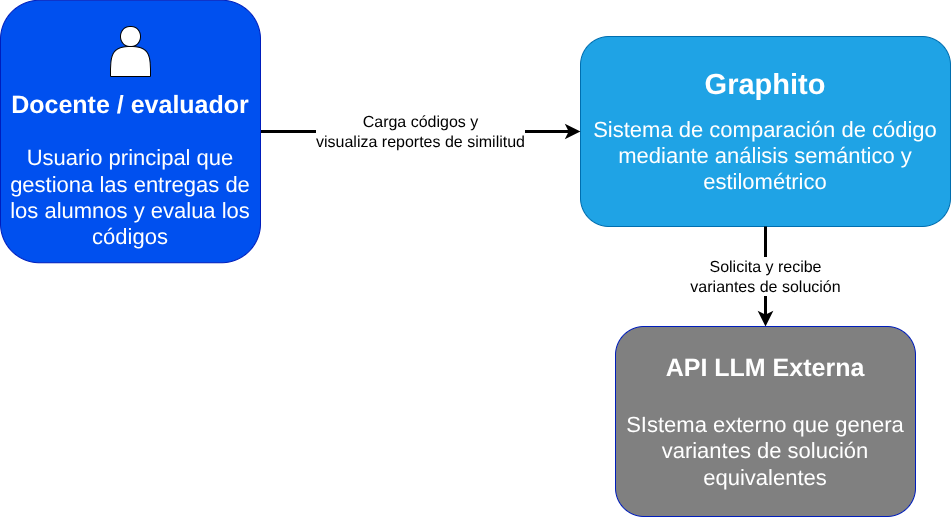
\includegraphics[width=1\textwidth]{figuras/diagrama_contexto.png}
    \caption{Diagrama de Contexto (Nivel 1) del sistema Graphito.}
    \label{fig:c4_contexto}
\end{figure}

\subsection{Nivel 2: Contenedores}

En este nivel de abstracción se detalla la arquitectura de micro-servicios y bases de datos que componen el sistema. \textit{Graphito} se separa funcionalmente en los siguientes contenedores principales:

\begin{itemize}
    \item \textbf{Capa de Cliente (Front-end):} Interfaz web interactiva en \textit{React} que consume servicios REST, facilitando el trabajo del docente.
    \item \textbf{Núcleo de Aplicación (Back-end):} Servicio principal implementado en \textit{FastAPI} (Python) encargado de orquestar el sistema, gestionar las peticiones a la IA y procesar la lógica general.
    \item \textbf{DB Relacional (PostgreSQL):} Persistencia estructurada para datos del usuario, problemas y registro histórico integral del análisis.
    \item \textbf{Vector DB (ChromaDB):} Persistencia hiperdimensional de los \textit{embeddings} que agilizan las búsquedas por proximidad semántica en las referencias.
\end{itemize}

\begin{figure}[H]
    \centering
    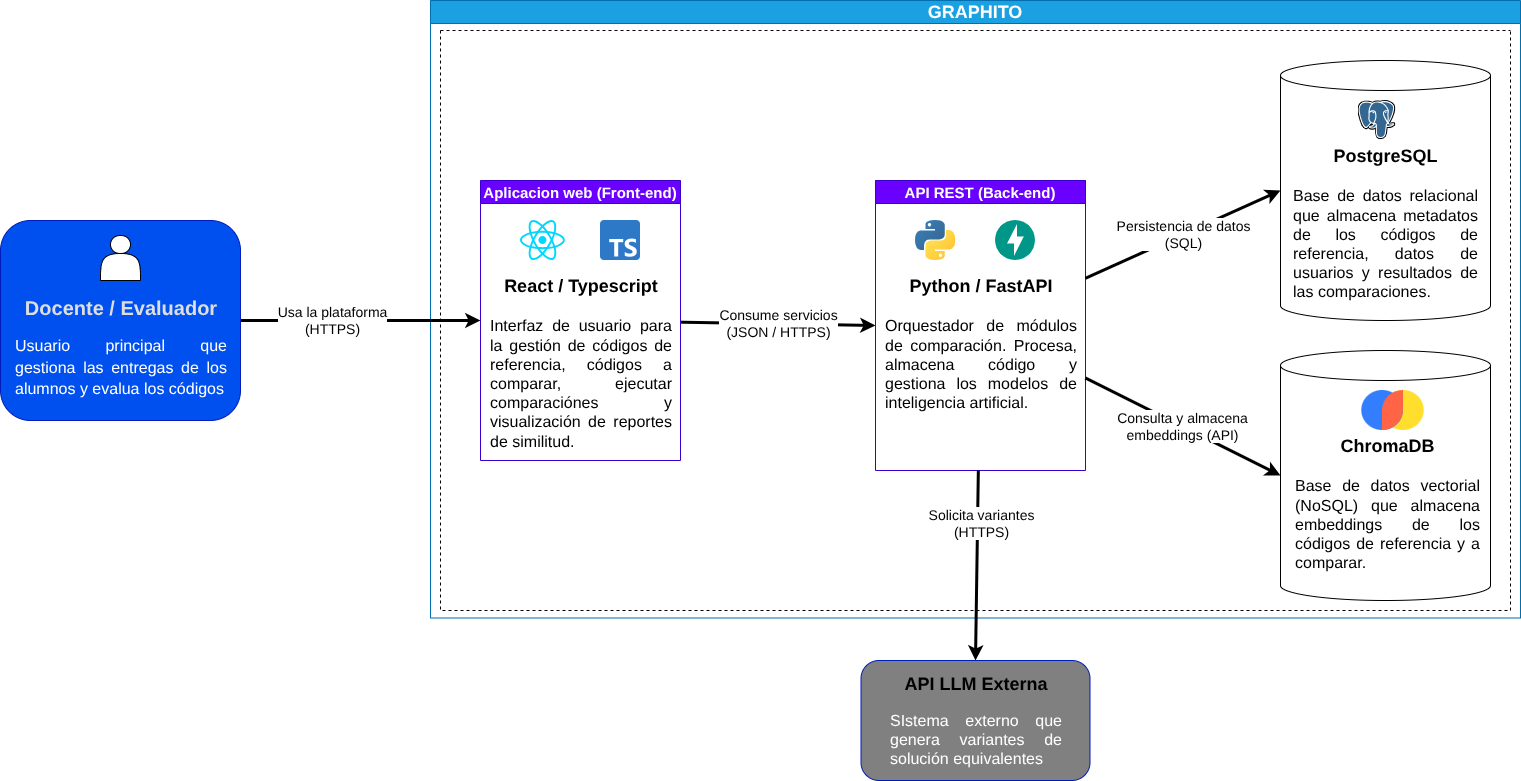
\includegraphics[width=1.0\textwidth]{figuras/diagrama_contenedores.png}
    \caption{Diagrama de Contenedores (Nivel 2) del sistema Graphito.}
    \label{fig:c4_contenedores}
\end{figure}

\subsection{Nivel 3: Componentes}

Haciendo un acercamiento al motor central de analítica del sistema (el contenedor Back-end de FastAPI), se ilustran los componentes internos que materializan la funcionalidad bimodal de auditoría académica para Graphito:

\begin{itemize}
    \item \textbf{Orquestador Inteligente (LangGraph):} Componente maestro de orquestación que evalúa iteraciones, fusiona características biomodales e interactúa cíclicamente para extender las referencias funcionales.
    \item \textbf{Módulo de Análisis Semántico:} Utiliza de forma profunda el modelo pre-entrenado \textit{GraphCodeBERT} para interpretar características lógicas a través del grafo de flujo de datos (DFG).
    \item \textbf{Módulo de Estilometría:} Implementa un clasificador \textit{CharCNN} a nivel de caracteres, capaz de categorizar autorías al aprender la textura de redacción original y capturar singularidades estructurales como sangrías o estilo de corchetes.
\end{itemize}

\begin{figure}[H]
    \centering
    % Placeholder sugerido
    %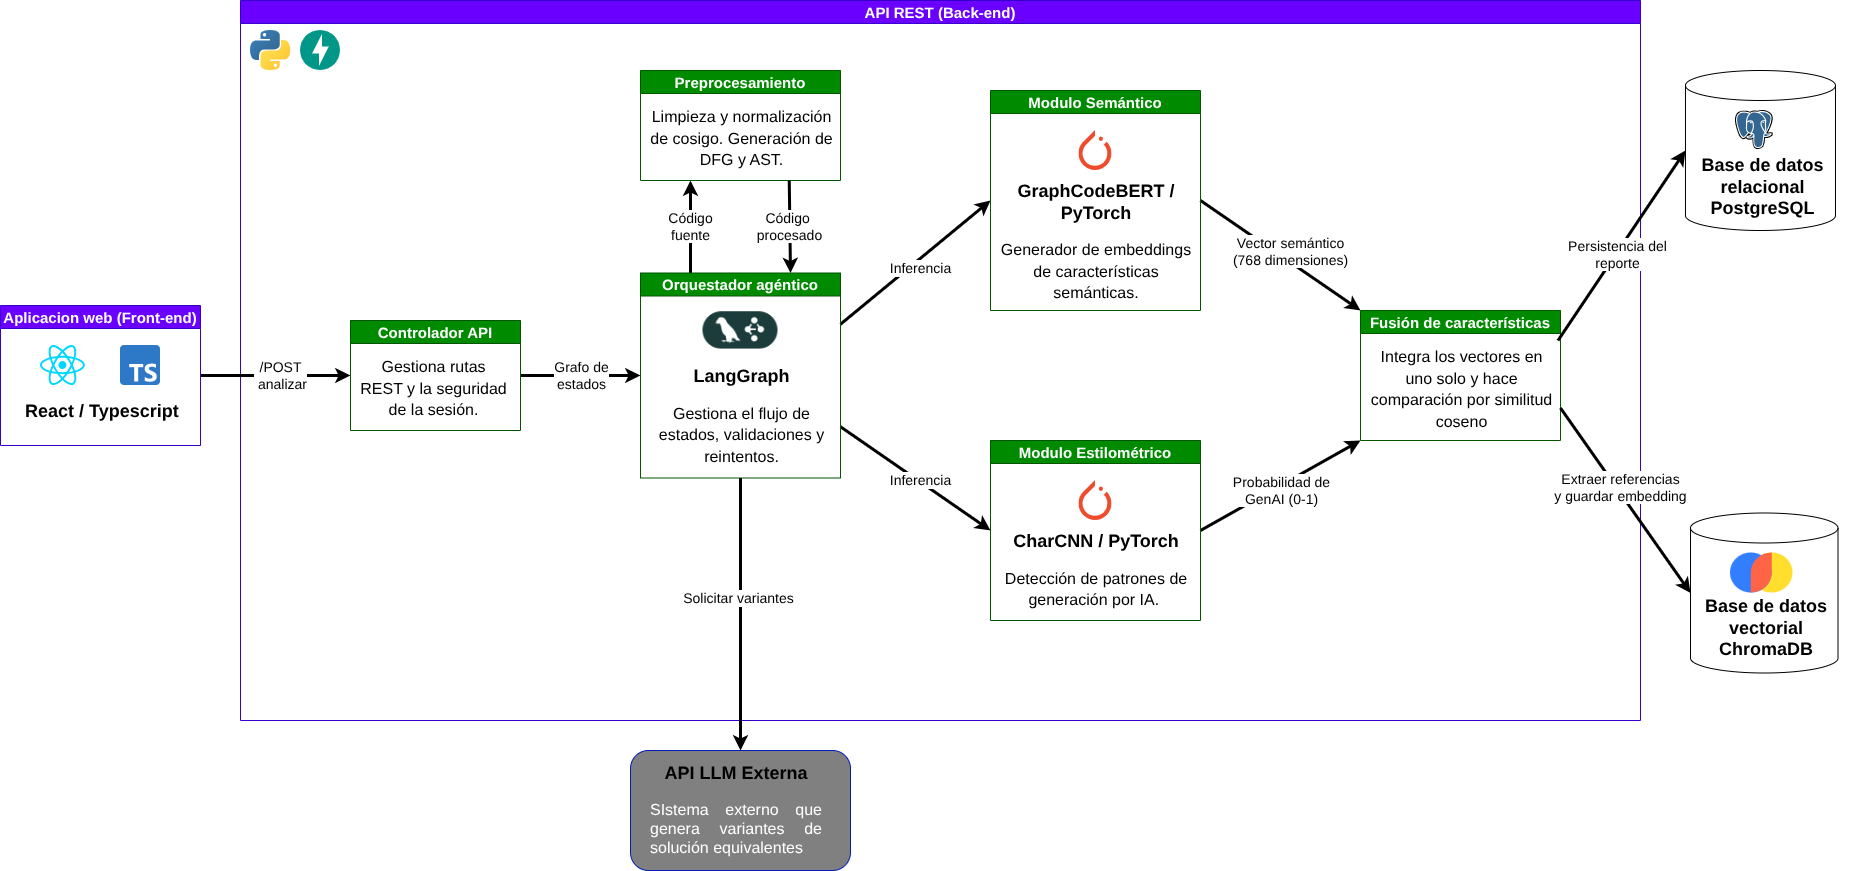
\includegraphics[width=0.8\textwidth]{figuras/diagrama_componentes.png}
    \caption{Diagrama de Componentes (Nivel 3) enfocado en el motor back-end en Python.}
    \label{fig:c4_componentes}
\end{figure}

\subsection{Nivel 4: Código (Clases y Secuencia)}

El nivel de código ofrece el máximo detalle referencial. Se subdivide en la vista estática, representada por las clases y patrones, y la vista dinámica, que muestra el paso a paso transaccional.

\subsubsection{Diagrama de Clases}

A nivel estático, el corazón del diseño obedece al patrón de diseño \textit{Strategy}. 

Como es posible constatar en el la Figura \ref{fig:diagrama_clases_graphito}, la ejecución transaccional principal se centraliza en \textbf{OrquestadorGraphito}, que coordina los módulos. El patrón \textit{Strategy} se aplica a la interfaz de inyección \textbf{ModeloIA}, separando los modelos predictivos como \textbf{ModeloGraphCodeBERT} y \textbf{ModeloCharCNN} del núcleo aplicativo. 

El componente \textbf{Preprocesador} bifurca el ciclo para proveer textos pulidos (análisis semántico) o crudos (estilométrico). Finalizada la ejecución iterativa, se concreta la \textbf{FirmaBimodal}. Por su parte, la persistencia se expone con la interfaz \textbf{AlmacenamientoDatos} la cual rige las lógicas independientes de \textbf{GestorPostgreSQL} y \textbf{GestorChromaDB}.

\begin{figure}[H]
    \centering
    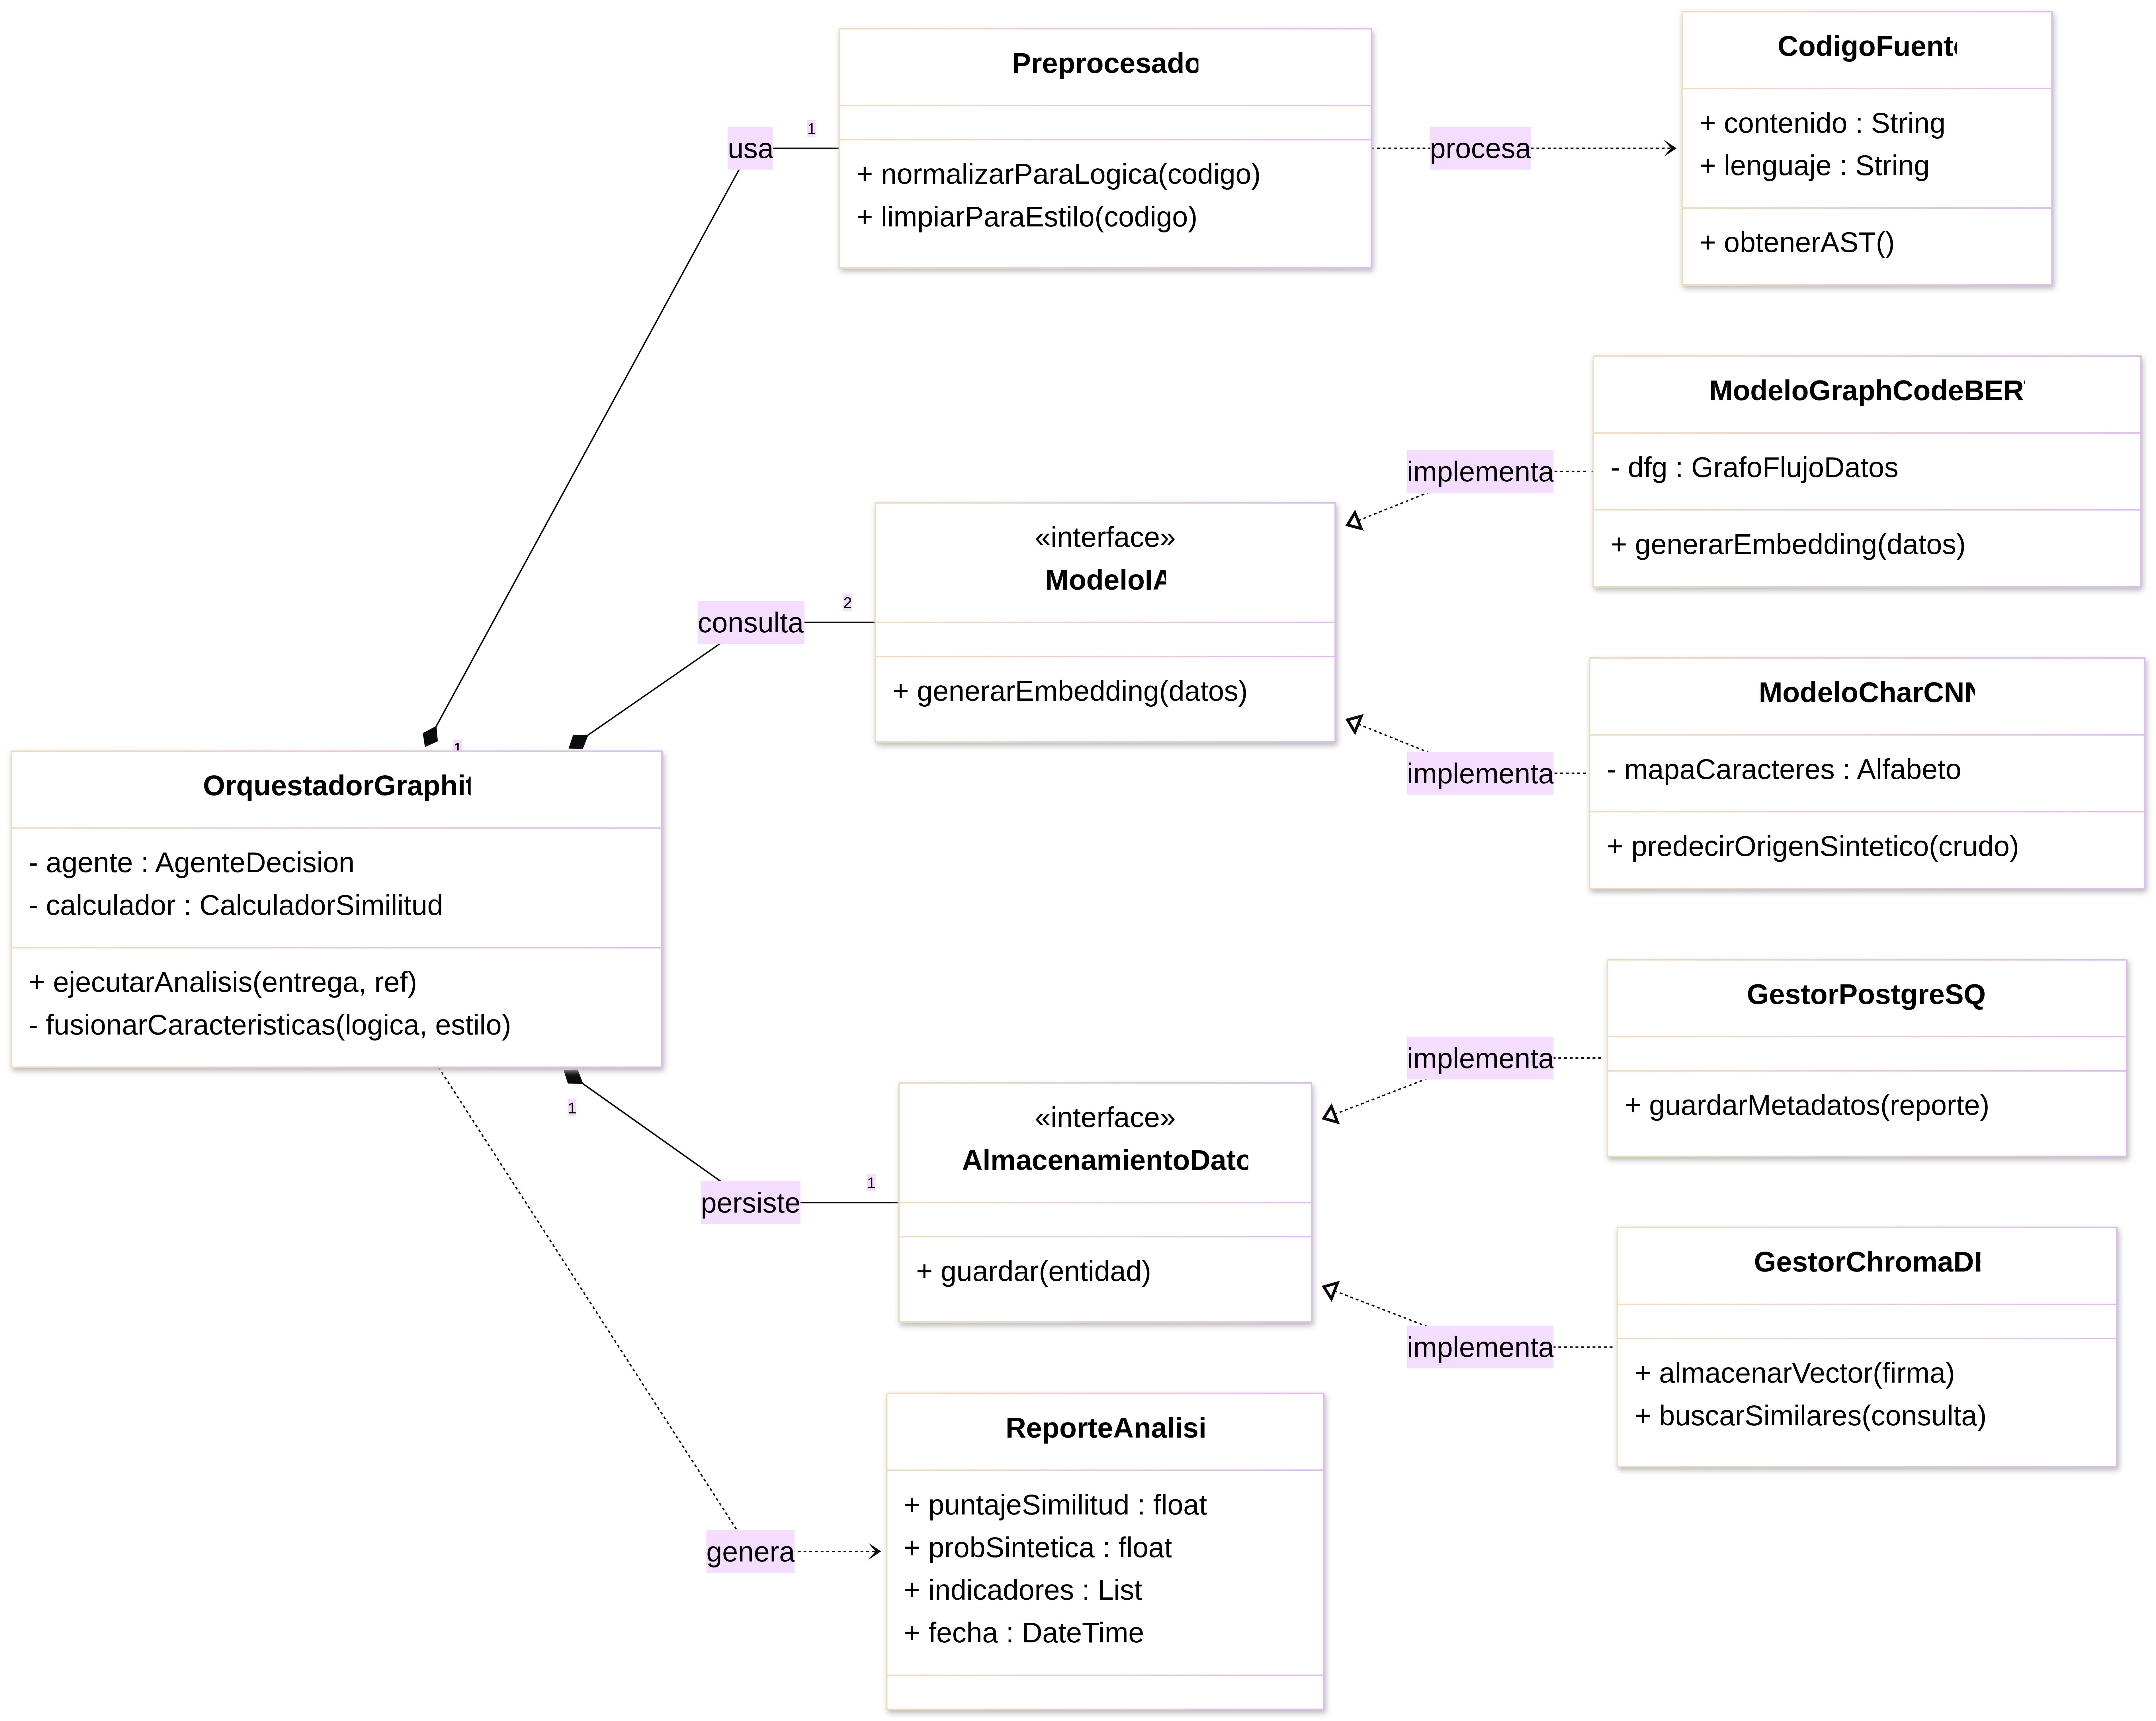
\includegraphics[width=\textwidth]{figuras/diagramaclases.png}
    \caption{Diagrama de clases del sistema Graphito, ilustrando la arquitectura orientada a objetos correspondientes al Nivel 4 de abstracción.}
    \label{fig:diagrama_clases_graphito}
\end{figure}

\subsubsection{Diagrama de Secuencia}

Para el flujo de eventos, el diagrama de secuencia dicta el actuar de los módulos durante una validación estándar:

\begin{itemize}
    \item \textbf{Ejecución Paralela:} Tanto GraphCodeBERT (para entender lógica) como CharCNN (para captar el perfil estilométrico) se ejecutan de manera concurrente con la finalidad de optimizar la inferencia. 
    \item \textbf{Veredicto y Alertas:} Una vez concatenado (\textit{early fusion}) el vector bimodal, se compara su similitud de coseno contra referencias maestras en ChromaDB y, bajo métricas específicas, se retornan las anomalías visuales a la capa de abstracción del frontend.
\end{itemize}

\begin{figure}[H]
    \centering
    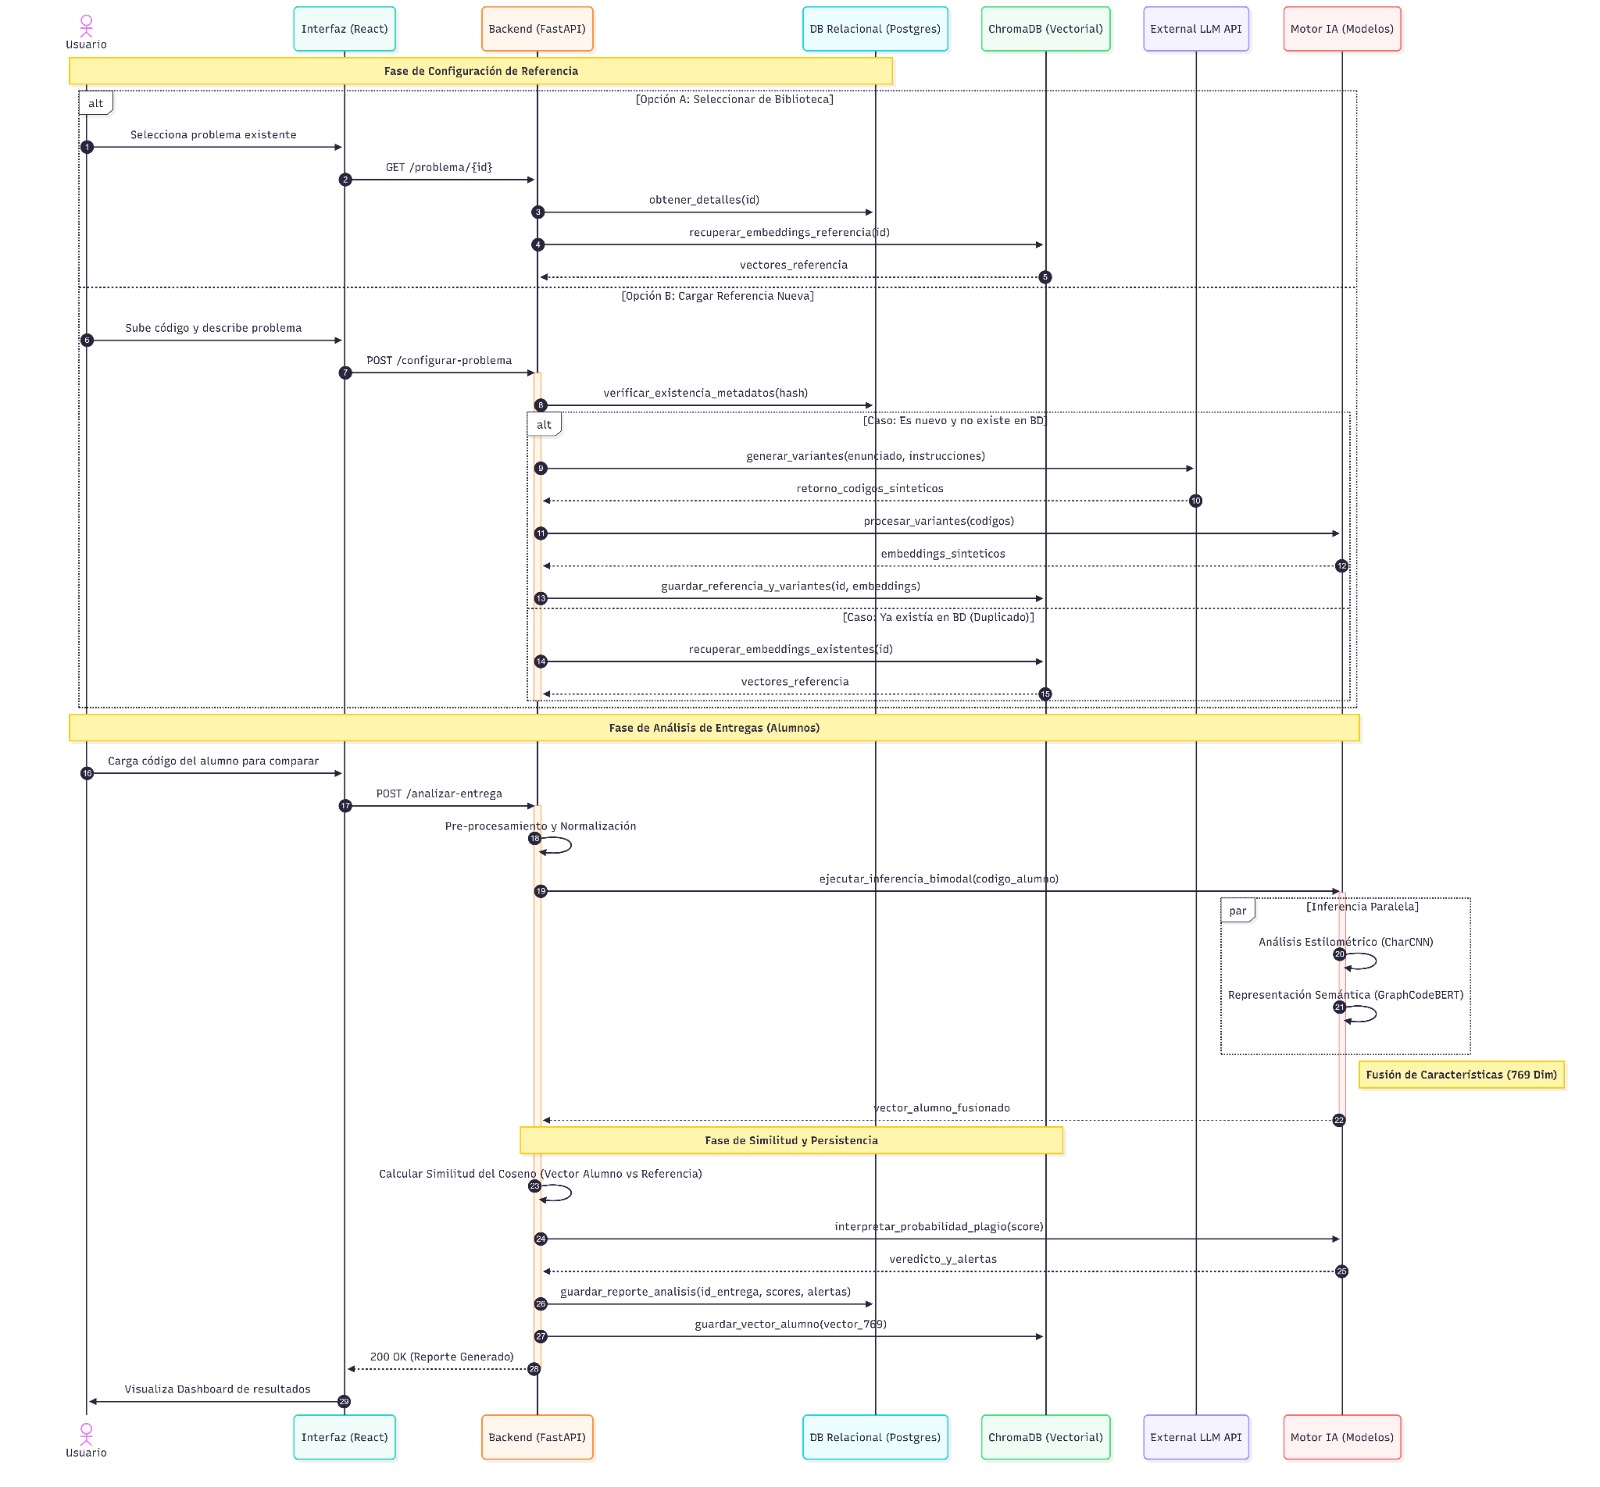
\includegraphics[width=0.9\textwidth]{figuras/diagramaSecuencia.jpeg}
    \caption{Diagrama de secuencia transaccional de \textit{Graphito} desde el cliente, Nivel 4.}
    \label{fig:diagrama_secuencia}
\end{figure}

% ---------------------------------------------------------
\section{Diseño de Base de Datos}
% ---------------------------------------------------------

Se ha implementado un sistema multi-persistencia (relacional y vectorial) para satisfacer requerimientos históricos y heurísticos.

\subsection{Modelo Relacional (Diagrama Entidad-Relación)}

El repositorio SQL maneja registros normalizados con PostgreSQL. Cada \textbf{DOCENTE} gestiona su entidad \textbf{PROBLEMA}. Dicha tabla posee cardinalidad con múltiples instancias de \textbf{CODIGO\_FUENTE} que documentan la entrega cruda en texto o las referencias de origen LLM y su metadata. 

Las similitudes y probabilidades resultantes tienen su hogar en la tabla transaccional \textbf{REPORTE\_ANALISIS}, la cual desencadena notificaciones a la entidad de \textbf{ALERTA\_INTEGRIDAD} al identificar comportamientos fuera del límite permisible en términos de completitud lógica versus artificialidad de estilo.

\begin{figure}[H]
    \centering
    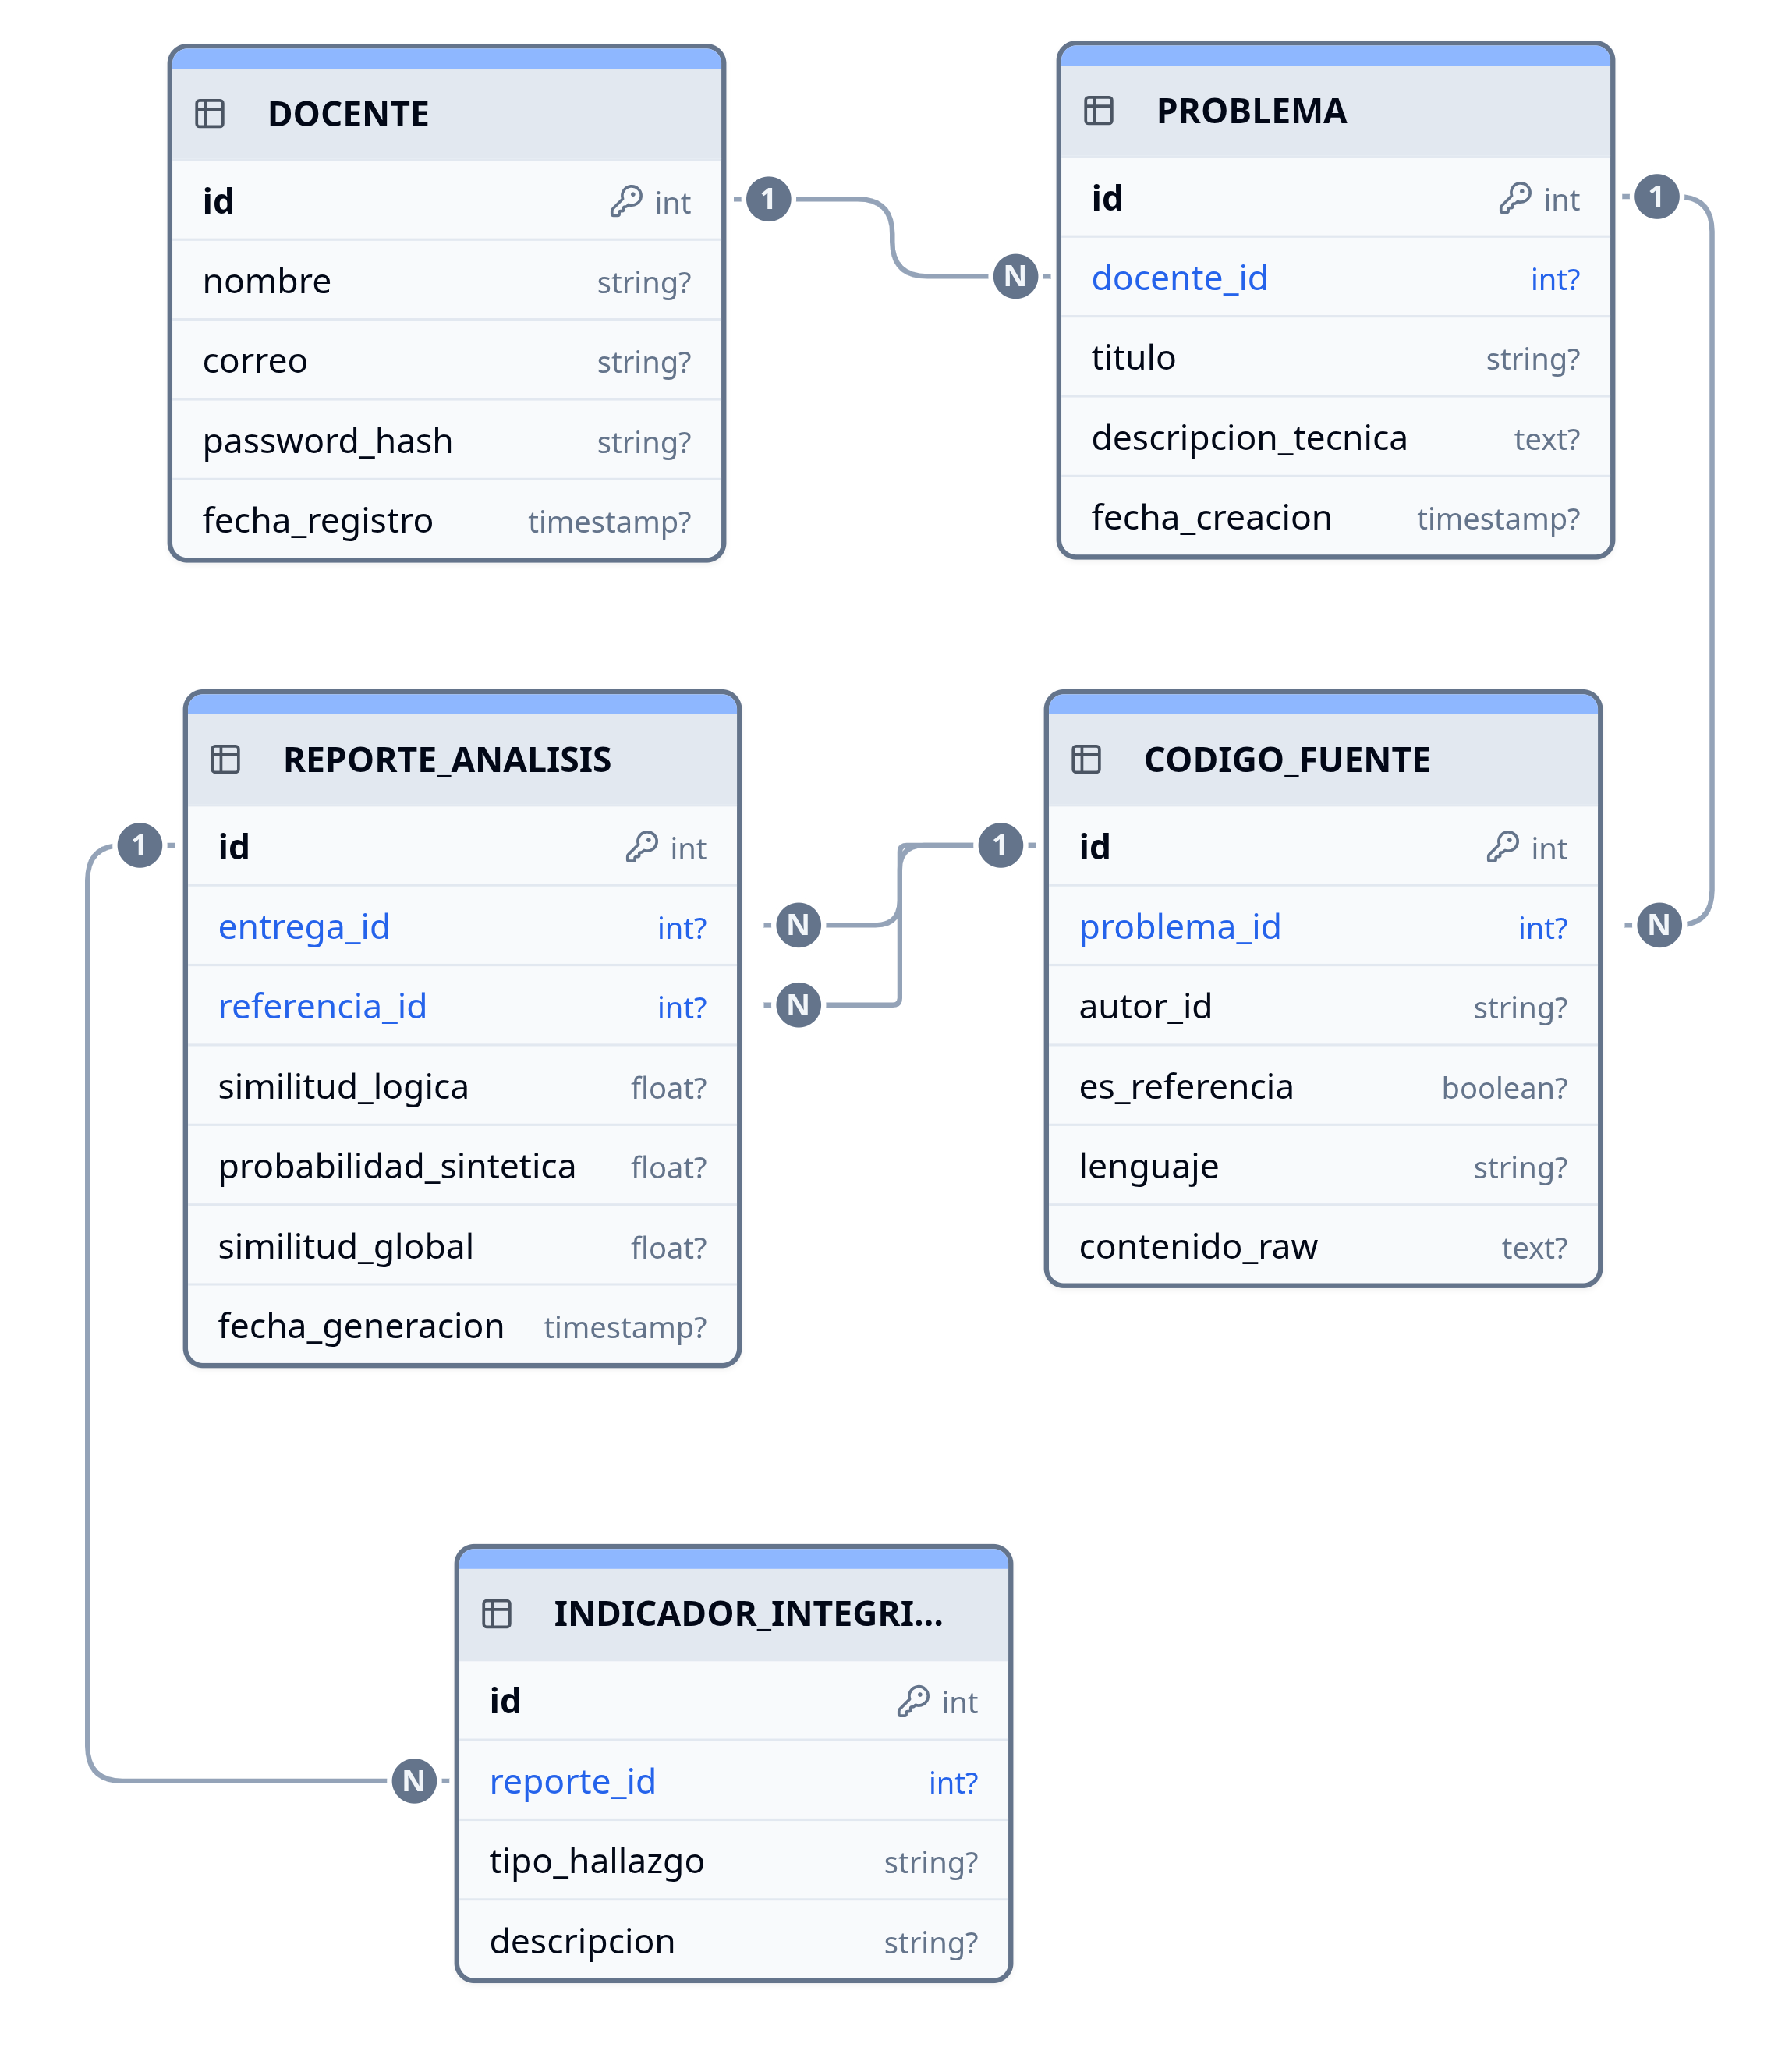
\includegraphics[width=\textwidth, height=0.75\textheight, keepaspectratio]{figuras/diagramarelacional.png}
    \caption{Diagrama C4 y Entidad-Relación de PostgreSQL sobre el componente integrador.}
    \label{fig:diagrama_er_graphito}
\end{figure}

\subsection{Esquema de Colección Vectorial (ChromaDB)}

La persistencia heurística se hospeda en el clúster transitorio o indexado de ChromaDB. Se estipuló un indexado central mediante la colección denominada \texttt{codigos\_referencia}, empleando UUIDs que coinciden con los registros almacenados en \texttt{CODIGO\_FUENTE} de su contraparte relacional.

Esta base vectorial aloja un \textit{embedding híbrido o concatenado} compuesto exactamente por \textbf{769 dimensiones}:
\begin{enumerate}
    \item \textbf{Dimensión [0 a 767] (Semántica):} Son formadas íntegramente por \textit{GraphCodeBERT} abstrayendo el comportamiento funcional del código.
    \item \textbf{Dimensión [768] (Estilometría):} Valor predictivo escalar inyectado desde la matriz \textit{CharCNN} donde se penaliza matemáticamente la autenticidad cuando los trazos reflejan una estructura sintética LLM.
\end{enumerate}

Para acelerar la segmentación del análisis de referencias, todos los nodos dentro de la colección ChromaDB se engloban con metadatos JSON básicos conteniendo al identificador de lógica (\texttt{problema\_id}), marcadores booleanos (\texttt{es\_referencia}), el ecosistema matriz como (\texttt{lenguaje}: \texttt{C|C++}) y un catalogador simple (\texttt{author\_type}).

% ---------------------------------------------------------
\section{Maquetación de la Interfaz}
% ---------------------------------------------------------

Para validar el análisis y diseño propuestos, se desarrollaron diferentes interfaces y componentes que conforman el prototipo inicial del sistema Graphito. A continuación, se documentan dichas pantallas, estableciendo la relación entre las vistas del sistema y los requerimientos funcionales definidos previamente.

\subsection{Arquitectura de Información}
La arquitectura de información del prototipo ha sido planteada para mantener un flujo intuitivo en la labor del docente. El sistema se compone de un área pública para la autenticación, y un área privada o "Centro de Mando" desde donde el usuario puede gestionar sus ejercicios, subir nuevas entregas y examinar los resultados del análisis semántico y estilométrico. Se prioriza una navegación jerárquica sencilla, facilitando el acceso a los reportes y comparaciones detalladas.

\subsection{Diseño de Interfaces (Pantallas)}

El diseño visual y funcional del prototipo aborda las principales necesidades del evaluador. A continuación, se presentan las diversas pantallas implementadas que demuestran el cumplimiento de los requerimientos de la plataforma.

\subsubsection{Inicio de Sesión y Registro}
El sistema cuenta con un área pública que permite a los docentes autenticarse y crear una cuenta, asegurando la privacidad de los ejercicios.

\begin{figure}[H]
    \centering
    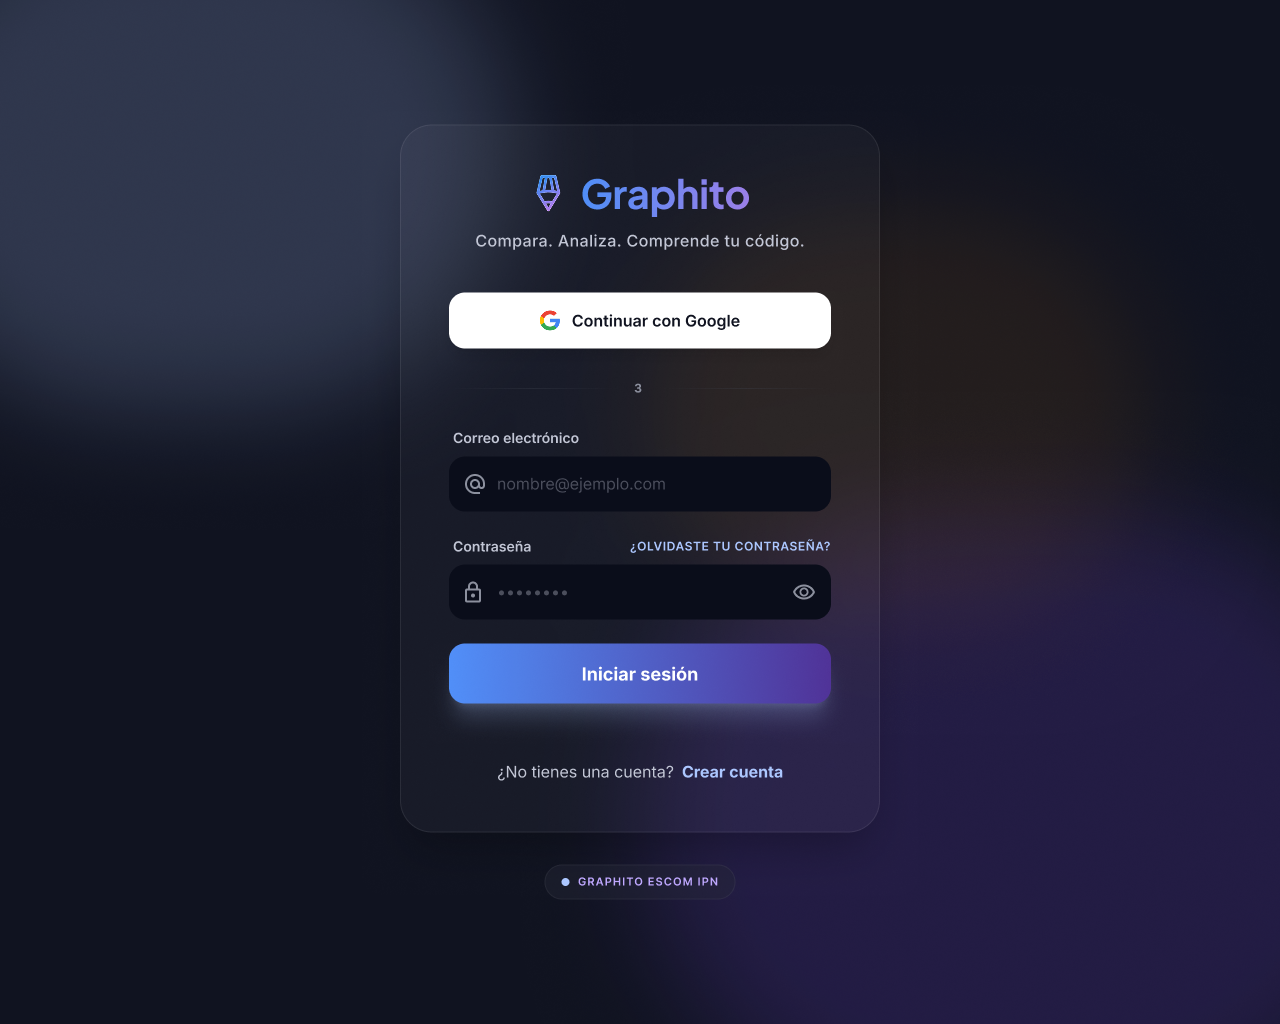
\includegraphics[width=0.8\textwidth]{figuras/iniciar_sesión.png}
    \caption{Interfaz de inicio de sesión, cumpliendo con el RF-01.}
    \label{fig:ui_iniciar_sesion}
\end{figure}

\begin{figure}[H]
    \centering
    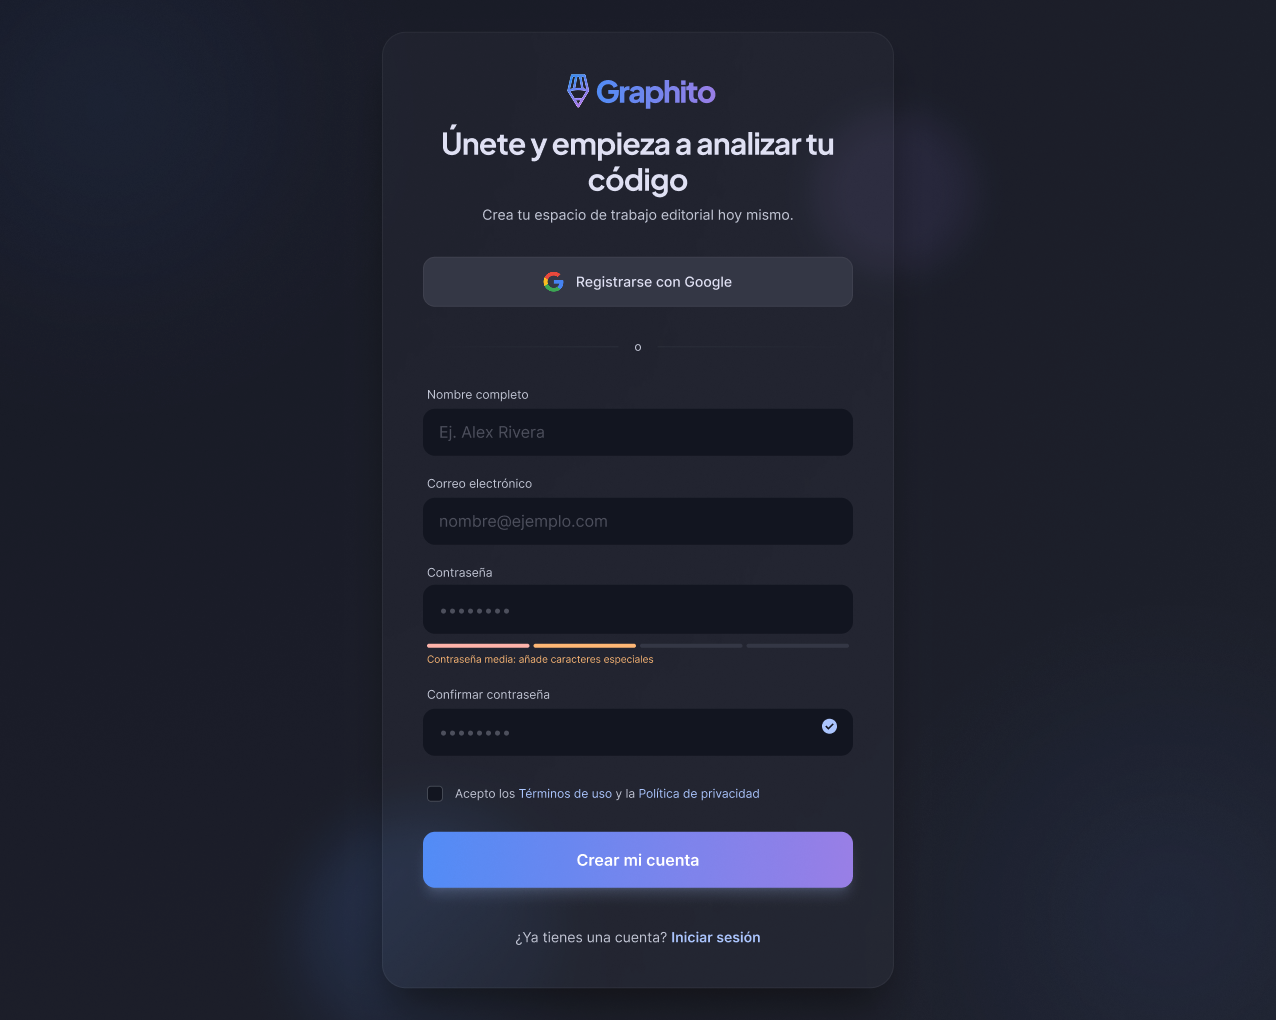
\includegraphics[width=0.8\textwidth]{figuras/crear_cuenta.png}
    \caption{Interfaz de creación de cuenta.}
    \label{fig:ui_crear_cuenta}
\end{figure}

\subsubsection{Interfaz de Carga de Código}
Se diseñó un mecanismo de carga sencillo para que los docentes integren nuevos archivos al sistema, agreguen comparaciones y comiencen el análisis automático de las entregas.

\begin{figure}[H]
    \centering
    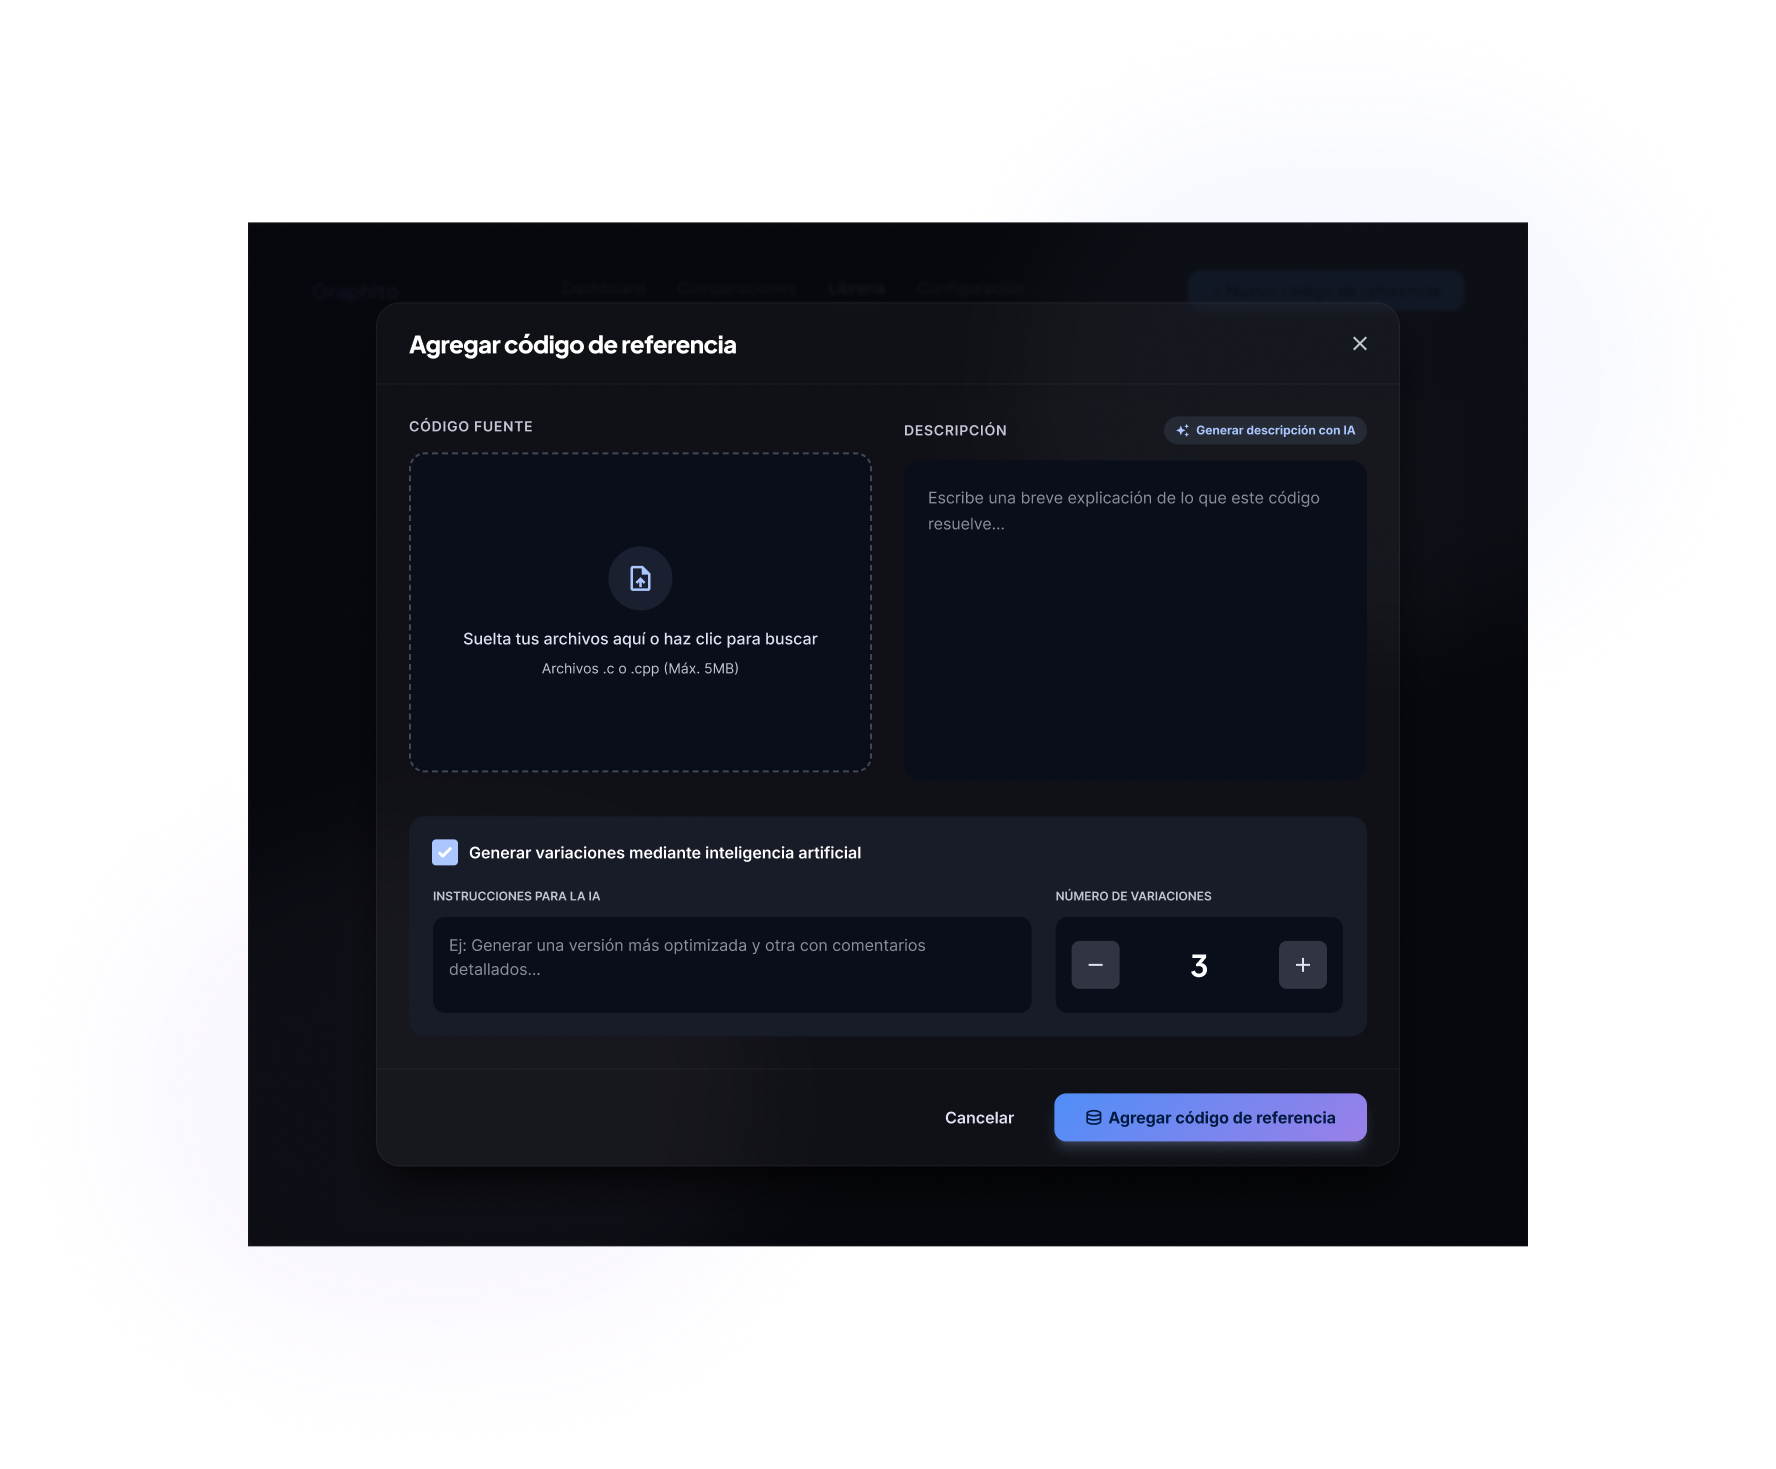
\includegraphics[width=0.8\textwidth]{figuras/nuevo_código_de_referencia.png}
    \caption{Interfaz para nuevo código de referencia, cumpliendo con el RF-03.}
    \label{fig:ui_carga_ref}
\end{figure}

\begin{figure}[H]
    \centering
    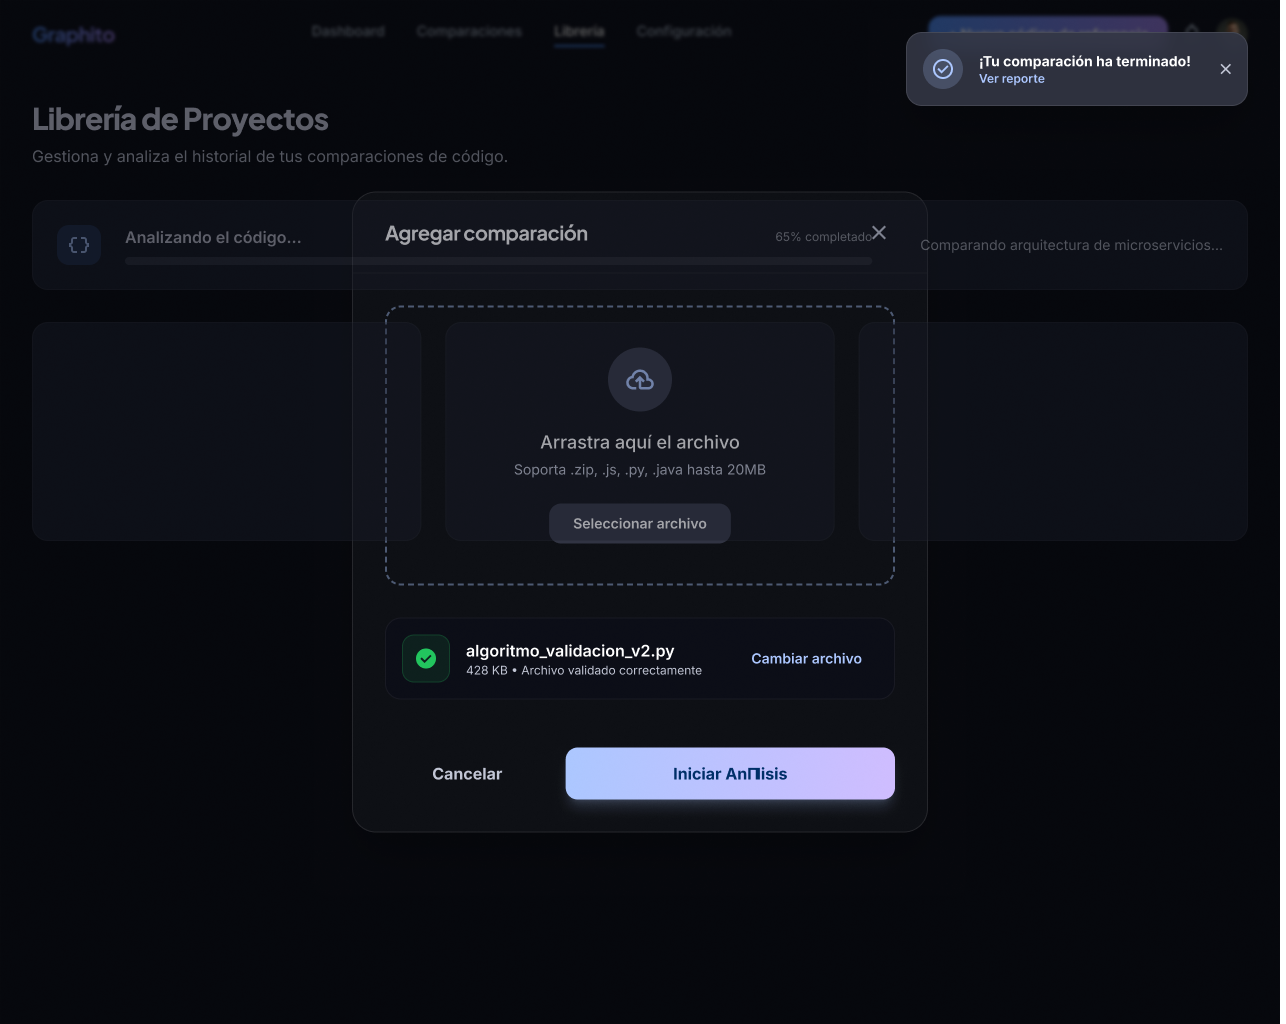
\includegraphics[width=0.8\textwidth]{figuras/agregar_comparación.png}
    \caption{Interfaz para agregar comparación.}
    \label{fig:ui_carga_comp}
\end{figure}

\subsubsection{Interfaz de Gestión y Repositorio}
Para organizar de manera efectiva el trabajo docente, el sistema cuenta con un repositorio personal de ejercicios.

\begin{figure}[H]
    \centering
    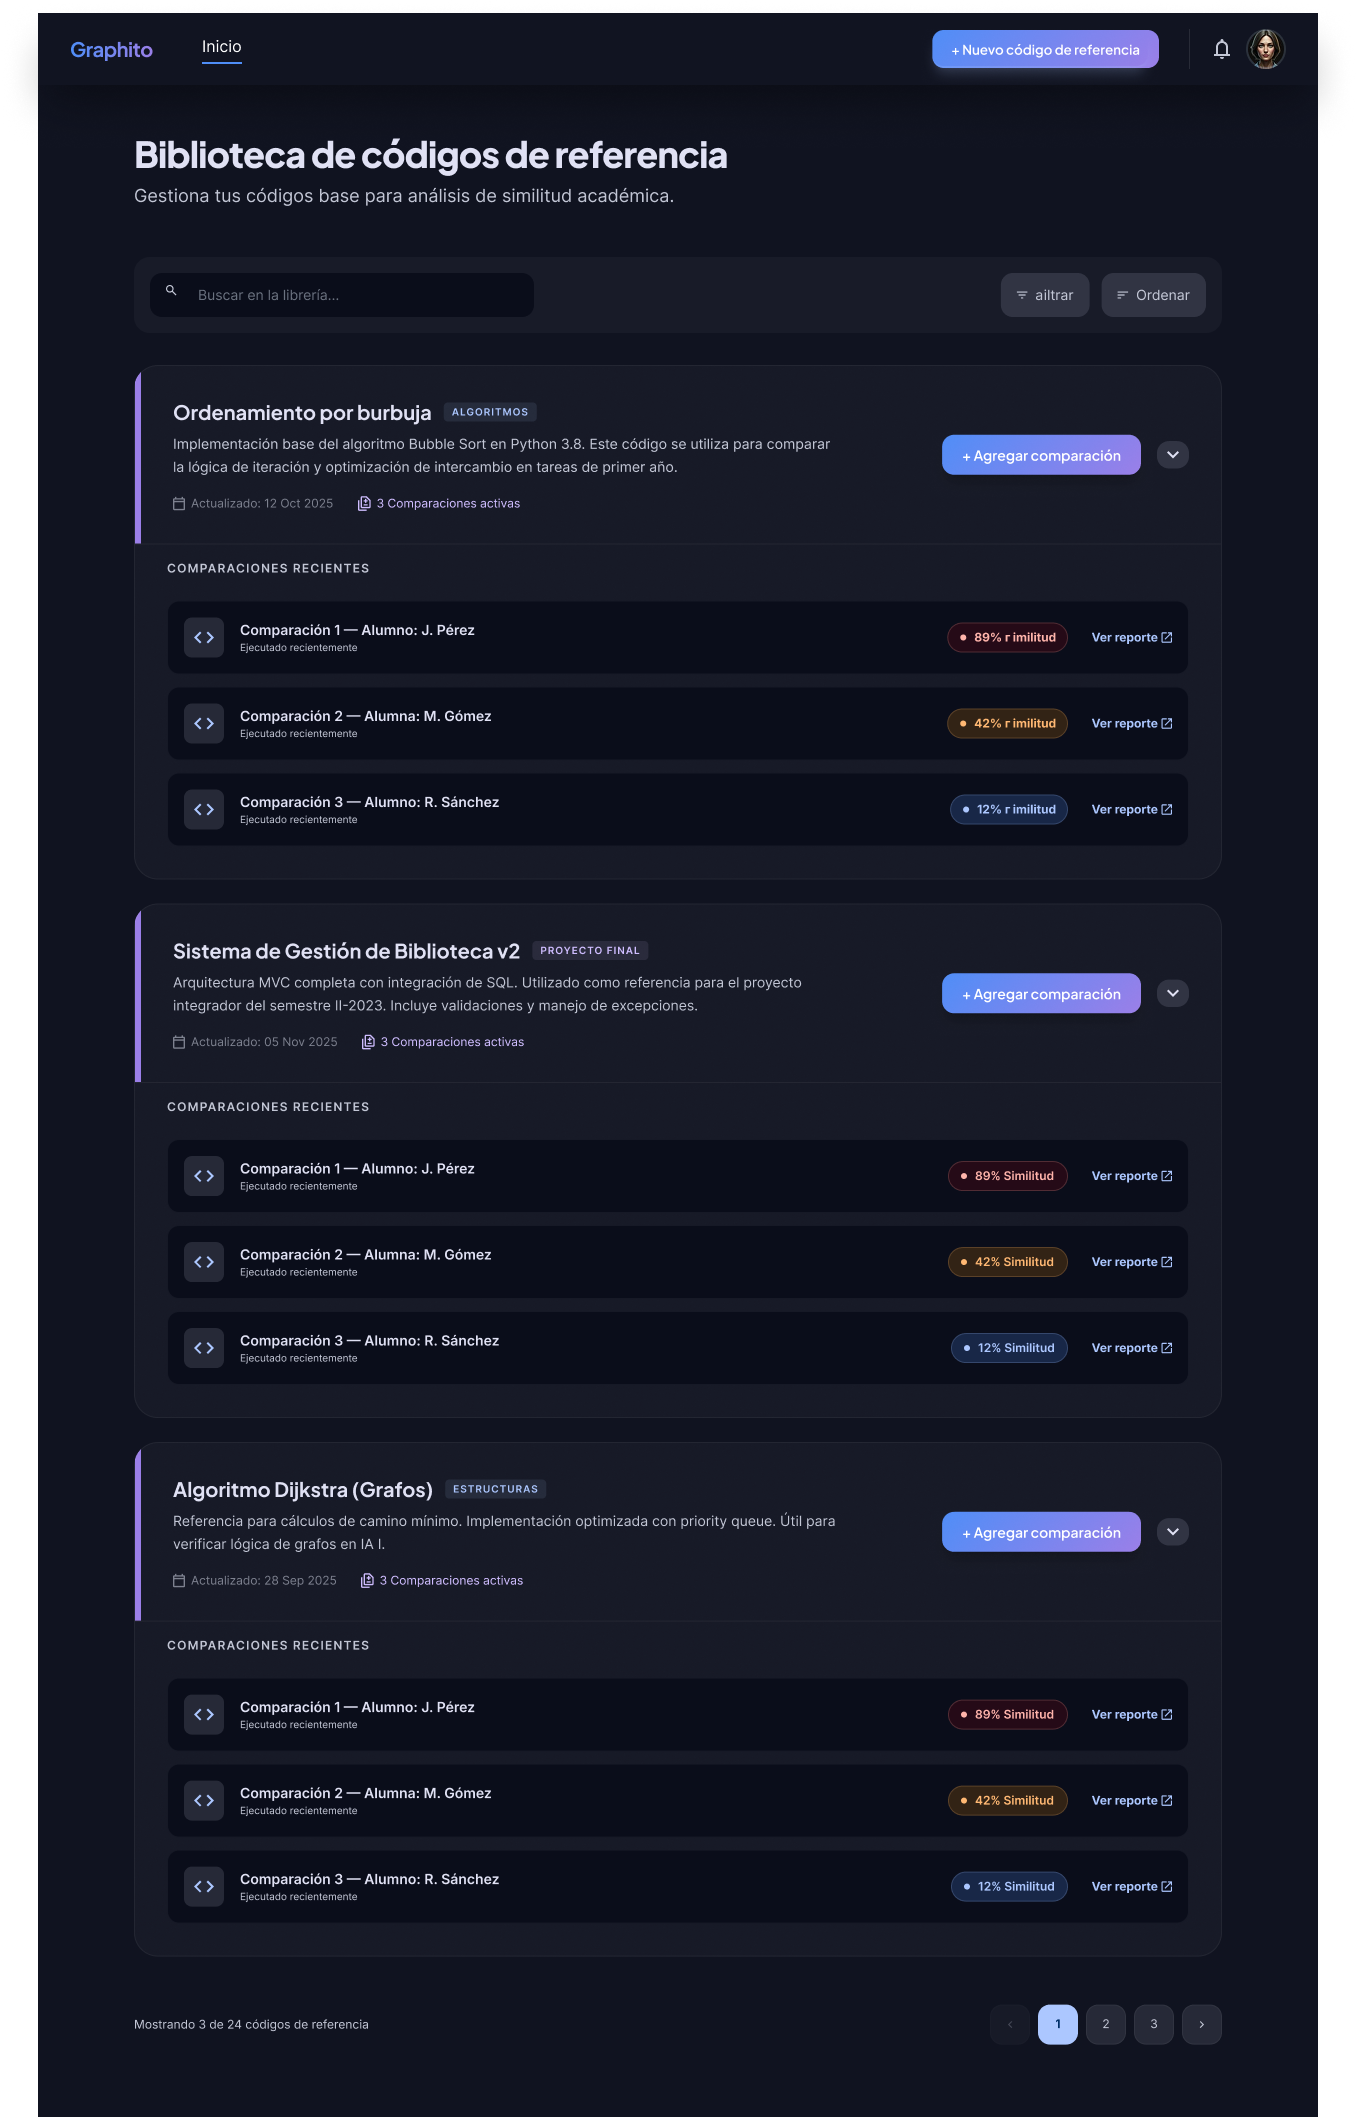
\includegraphics[width=0.8\textwidth]{figuras/biblioteca_de_referencias.png}
    \caption{Repositorio personal de ejercicios, cumpliendo con el RF-02.}
    \label{fig:ui_repositorio}
\end{figure}

El \textbf{RF-02} especifica que el sistema debe permitir al docente la creación y gestión de un listado de ejercicios o problemas de programación. La Figura \ref{fig:ui_repositorio} muestra la implementación de esta funcionalidad, ofreciendo una vista consolidada de los problemas registrados.

\subsubsection{Reporte de Análisis Bimodal}
La pantalla principal de resultados presenta de forma integral las métricas calculadas por los motores de inteligencia artificial.

\begin{figure}[H]
    \centering
    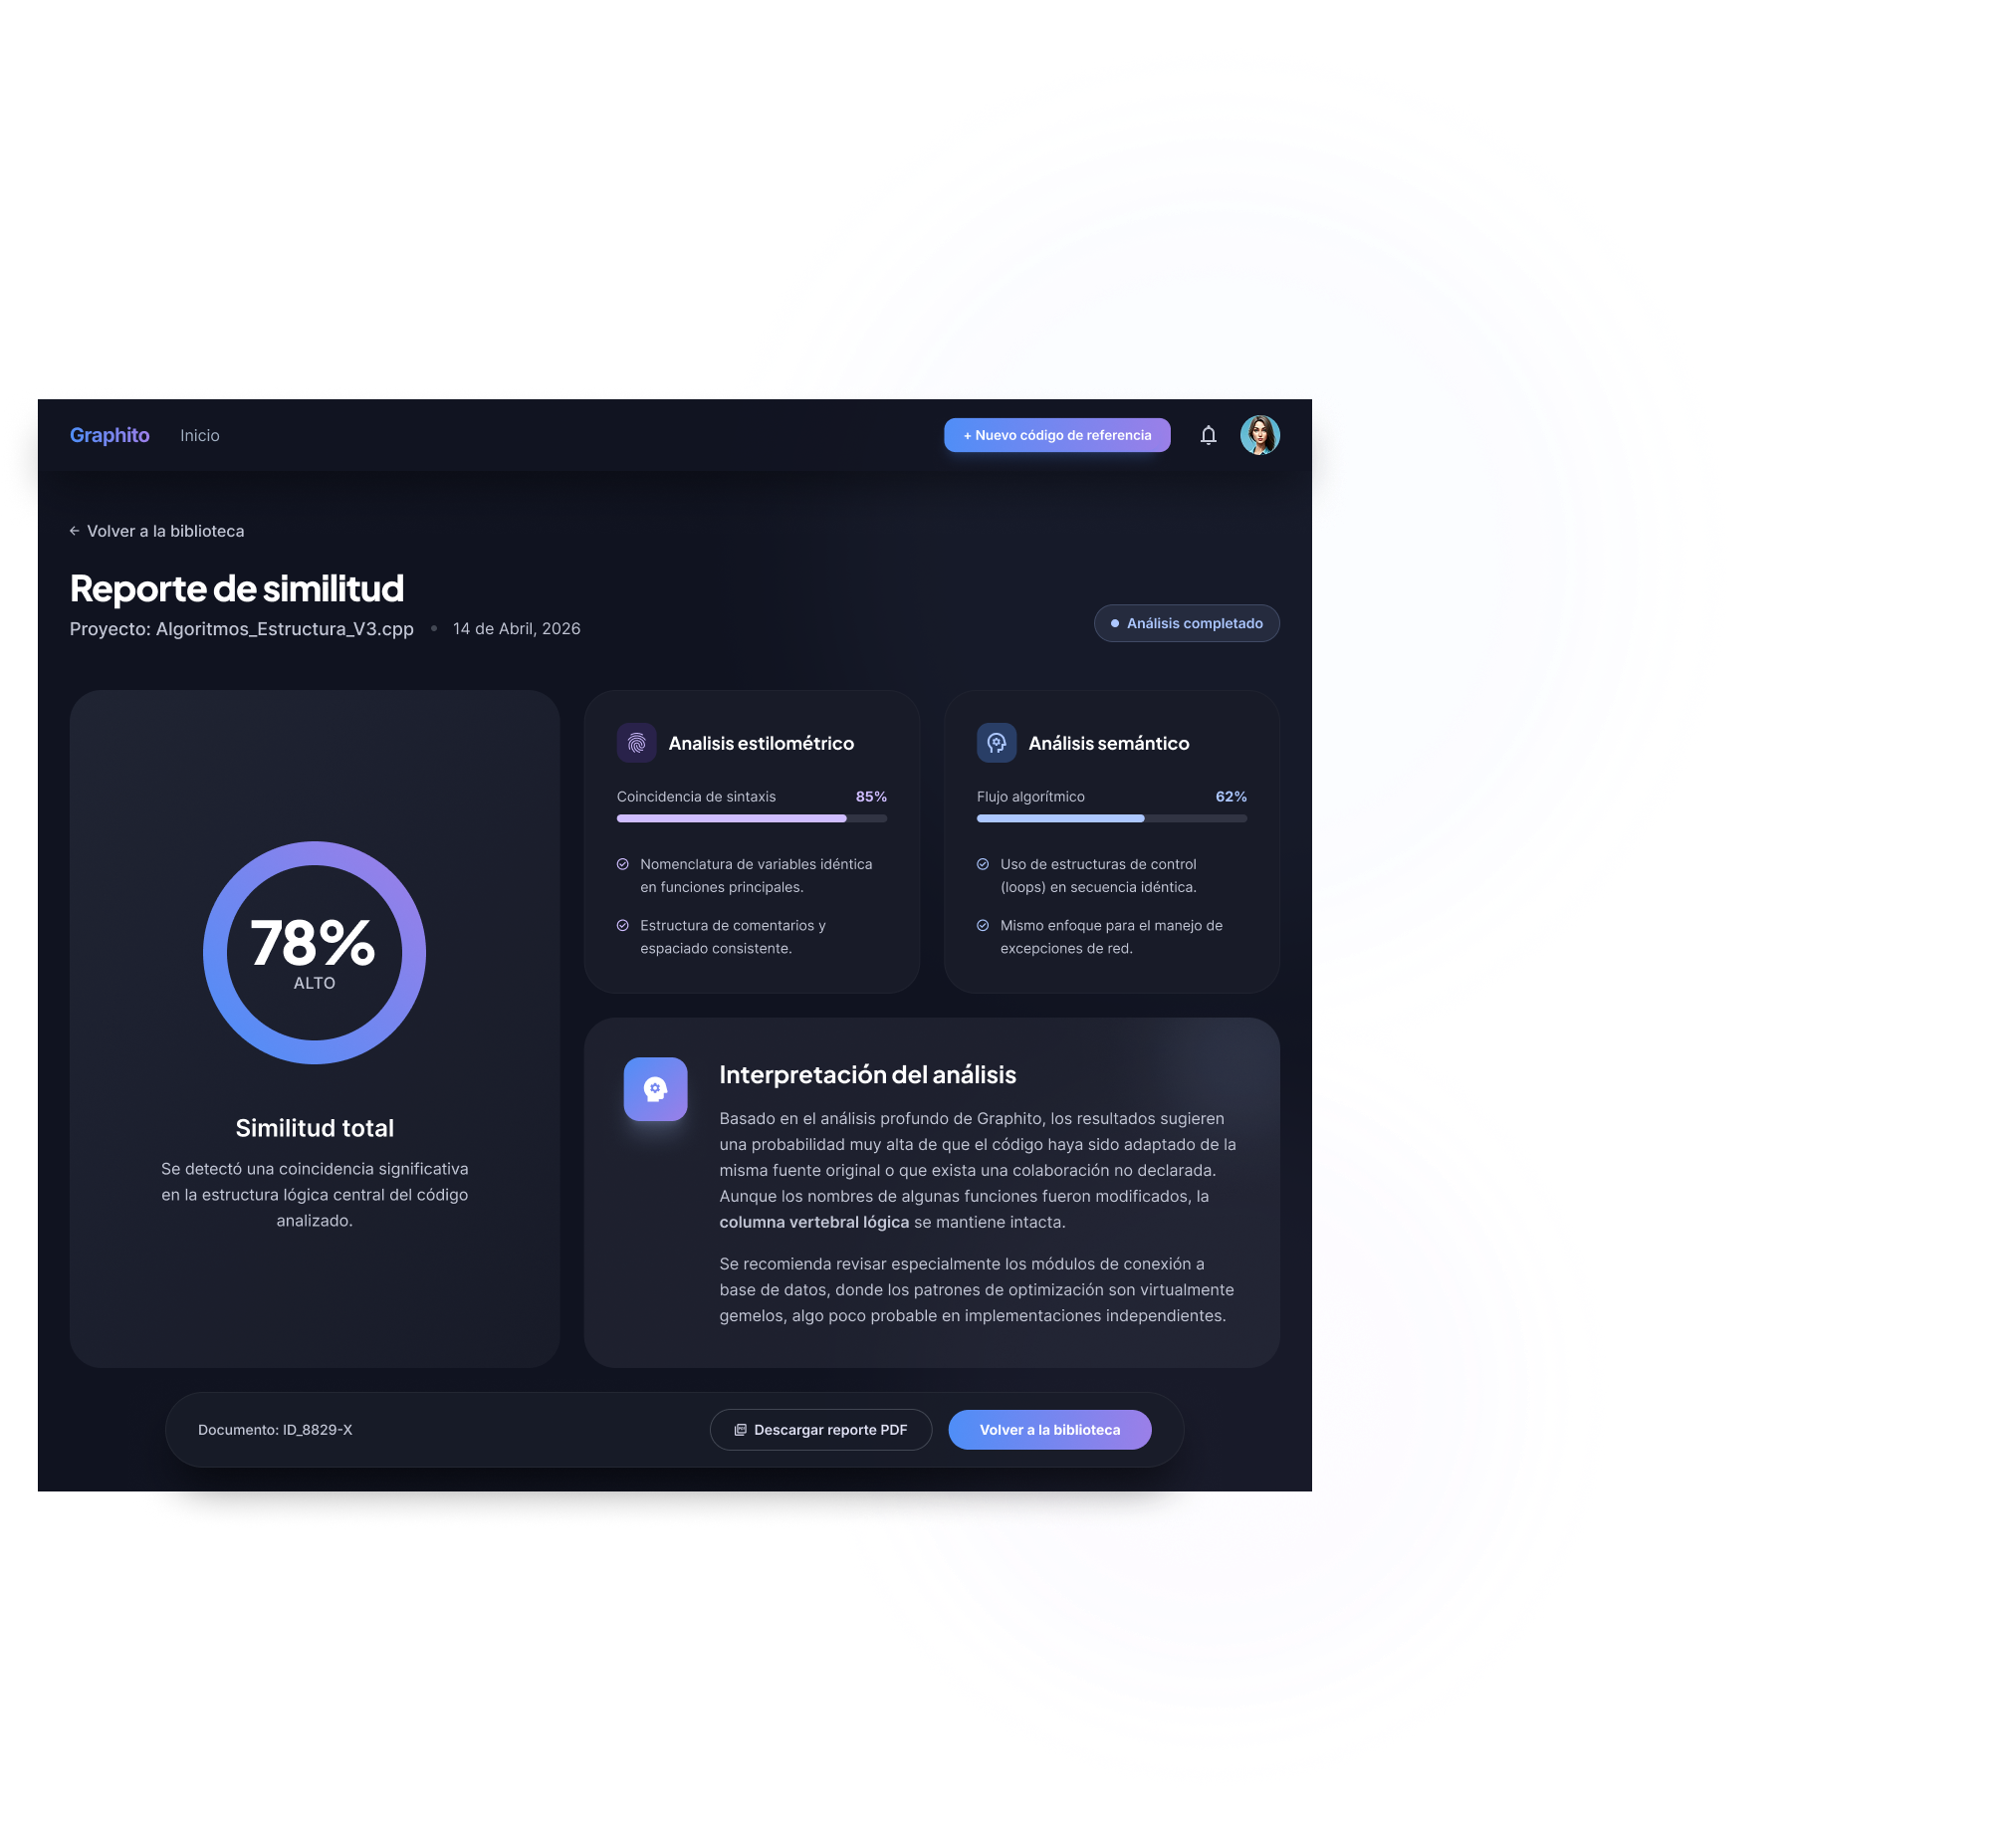
\includegraphics[width=0.8\textwidth]{figuras/reporte_de_similitud.png}
    \caption{Dashboard de reporte bimodal, cumpliendo con el RF-10 y RF-11.}
    \label{fig:ui_reporte}
\end{figure}

En la Figura \ref{fig:ui_reporte} se visualiza la interfaz del reporte, cumpliendo con el \textbf{RF-10} sobre la necesidad de generar un reporte bimodal que integre el índice de similitud semántica y la probabilidad de autoría de forma visual. Además, esta pantalla despliega de manera automática las alertas de integridad estipuladas en el \textbf{RF-11} frente a discrepancias entre la lógica y el estilo.
 

% --- REFERENCIAS ---
\newpage
\addcontentsline{toc}{chapter}{Referencias}
\bibliographystyle{IEEEtran}
\bibliography{referencias}

\end{document}